\documentclass[twoside]{book}

% Packages required by doxygen
\usepackage{fixltx2e}
\usepackage{calc}
\usepackage{doxygen}
\usepackage[export]{adjustbox} % also loads graphicx
\usepackage{graphicx}
\usepackage[utf8]{inputenc}
\usepackage{makeidx}
\usepackage{multicol}
\usepackage{multirow}
\PassOptionsToPackage{warn}{textcomp}
\usepackage{textcomp}
\usepackage[nointegrals]{wasysym}
\usepackage[table]{xcolor}

% NLS support packages
Portuguese
% Font selection
\usepackage[T1]{fontenc}
\usepackage[scaled=.90]{helvet}
\usepackage{courier}
\usepackage{amssymb}
\usepackage{sectsty}
\renewcommand{\familydefault}{\sfdefault}
\allsectionsfont{%
  \fontseries{bc}\selectfont%
  \color{darkgray}%
}
\renewcommand{\DoxyLabelFont}{%
  \fontseries{bc}\selectfont%
  \color{darkgray}%
}
\newcommand{\+}{\discretionary{\mbox{\scriptsize$\hookleftarrow$}}{}{}}

% Page & text layout
\usepackage{geometry}
\geometry{%
  a4paper,%
  top=2.5cm,%
  bottom=2.5cm,%
  left=2.5cm,%
  right=2.5cm%
}
\tolerance=750
\hfuzz=15pt
\hbadness=750
\setlength{\emergencystretch}{15pt}
\setlength{\parindent}{0cm}
\setlength{\parskip}{3ex plus 2ex minus 2ex}
\makeatletter
\renewcommand{\paragraph}{%
  \@startsection{paragraph}{4}{0ex}{-1.0ex}{1.0ex}{%
    \normalfont\normalsize\bfseries\SS@parafont%
  }%
}
\renewcommand{\subparagraph}{%
  \@startsection{subparagraph}{5}{0ex}{-1.0ex}{1.0ex}{%
    \normalfont\normalsize\bfseries\SS@subparafont%
  }%
}
\makeatother

% Headers & footers
\usepackage{fancyhdr}
\pagestyle{fancyplain}
\fancyhead[LE]{\fancyplain{}{\bfseries\thepage}}
\fancyhead[CE]{\fancyplain{}{}}
\fancyhead[RE]{\fancyplain{}{\bfseries\leftmark}}
\fancyhead[LO]{\fancyplain{}{\bfseries\rightmark}}
\fancyhead[CO]{\fancyplain{}{}}
\fancyhead[RO]{\fancyplain{}{\bfseries\thepage}}
\fancyfoot[LE]{\fancyplain{}{}}
\fancyfoot[CE]{\fancyplain{}{}}
\fancyfoot[RE]{\fancyplain{}{\bfseries\scriptsize Gerado por Doxygen }}
\fancyfoot[LO]{\fancyplain{}{\bfseries\scriptsize Gerado por Doxygen }}
\fancyfoot[CO]{\fancyplain{}{}}
\fancyfoot[RO]{\fancyplain{}{}}
\renewcommand{\footrulewidth}{0.4pt}
\renewcommand{\chaptermark}[1]{%
  \markboth{#1}{}%
}
\renewcommand{\sectionmark}[1]{%
  \markright{\thesection\ #1}%
}

% Indices & bibliography
\usepackage{natbib}
\usepackage[titles]{tocloft}
\setcounter{tocdepth}{3}
\setcounter{secnumdepth}{5}
\makeindex

% Hyperlinks (required, but should be loaded last)
\usepackage{ifpdf}
\ifpdf
  \usepackage[pdftex,pagebackref=true]{hyperref}
\else
  \usepackage[ps2pdf,pagebackref=true]{hyperref}
\fi
\hypersetup{%
  colorlinks=true,%
  linkcolor=blue,%
  citecolor=blue,%
  unicode%
}

% Custom commands
\newcommand{\clearemptydoublepage}{%
  \newpage{\pagestyle{empty}\cleardoublepage}%
}

\usepackage{caption}
\captionsetup{labelsep=space,justification=centering,font={bf},singlelinecheck=off,skip=4pt,position=top}

%===== C O N T E N T S =====

\begin{document}

% Titlepage & ToC
\hypersetup{pageanchor=false,
             bookmarksnumbered=true,
             pdfencoding=unicode
            }
\pagenumbering{alph}
\begin{titlepage}
\vspace*{7cm}
\begin{center}%
{\Large Graph\+O\+DA }\\
\vspace*{1cm}
{\large Gerado por Doxygen 1.8.13}\\
\end{center}
\end{titlepage}
\clearemptydoublepage
\pagenumbering{roman}
\tableofcontents
\clearemptydoublepage
\pagenumbering{arabic}
\hypersetup{pageanchor=true}

%--- Begin generated contents ---
\chapter{2019-\/1-\/grupo19}
\label{index}\hypertarget{index}{}\href{https://travis-ci.com/pds2-dcc-ufmg/2019-1-grupo19}{\texttt{ }}\hypertarget{index_autotoc_md1}{}\doxysection{Como instalar as dependências?}\label{index_autotoc_md1}
Um script simples para Ubuntu 18.\+04+ 
\begin{DoxyCode}{0}
\DoxyCodeLine{sudo add-\/apt-\/repository ppa:texus/tgui-\/0.8}
\DoxyCodeLine{sudo apt-\/get update}
\DoxyCodeLine{sudo apt-\/get install libsfml-\/dev libtgui-\/dev}
\end{DoxyCode}
\hypertarget{index_autotoc_md2}{}\doxysection{Como desenvolver localmente?}\label{index_autotoc_md2}

\begin{DoxyCode}{0}
\DoxyCodeLine{\# Gere os scripts de compilação para sua plataforma}
\DoxyCodeLine{cmake CMakeLists.txt}
\DoxyCodeLine{\# Compile}
\DoxyCodeLine{make}
\DoxyCodeLine{\# Execute}
\DoxyCodeLine{./graphODA}
\end{DoxyCode}
\hypertarget{index_autotoc_md3}{}\doxysection{Como usar o R\+E\+PL}\label{index_autotoc_md3}
O R\+E\+PL possui dois tipos de comando\+: atribuição e operação.\hypertarget{index_autotoc_md4}{}\doxysubsection{Atribuição}\label{index_autotoc_md4}
\hypertarget{index_autotoc_md5}{}\doxysubsubsection{Atribuição de variável}\label{index_autotoc_md5}

\begin{DoxyCode}{0}
\DoxyCodeLine{>>> var1 = var2}
\end{DoxyCode}
 A variável {\itshape var1} passa a representar o grafo representado por {\itshape var2}.\hypertarget{index_autotoc_md6}{}\doxysubsubsection{import}\label{index_autotoc_md6}

\begin{DoxyCode}{0}
\DoxyCodeLine{>>> var = import file\_name}
\end{DoxyCode}
 A variável {\itshape var} passa a representar o grafo armazenado em {\itshape file\+\_\+name}. Se a leitura do arquivo falhar, {\itshape var} passa a representar um grafo vazio.\hypertarget{index_autotoc_md7}{}\doxysubsubsection{mst}\label{index_autotoc_md7}

\begin{DoxyCode}{0}
\DoxyCodeLine{>>> var1 = mst var2}
\end{DoxyCode}
 A variável {\itshape var1} passa a representar a {\bfseries{árvore geradora mínima}} do grafo representado por {\itshape var2}.\hypertarget{index_autotoc_md8}{}\doxysubsection{Operação}\label{index_autotoc_md8}
\hypertarget{index_autotoc_md9}{}\doxysubsubsection{describe}\label{index_autotoc_md9}

\begin{DoxyCode}{0}
\DoxyCodeLine{>>> var > describe}
\end{DoxyCode}
 Exibe informações sobre o grafo representado por {\itshape var}.\hypertarget{index_autotoc_md10}{}\doxysubsubsection{show}\label{index_autotoc_md10}

\begin{DoxyCode}{0}
\DoxyCodeLine{>>> var > show}
\end{DoxyCode}
 Exibe o grafo representado por {\itshape var}.\hypertarget{index_autotoc_md11}{}\doxysubsubsection{edit}\label{index_autotoc_md11}

\begin{DoxyCode}{0}
\DoxyCodeLine{>>> var > edit}
\end{DoxyCode}
 Exibe o grafo representado por {\itshape var}, salvando as modificações efetuadas.\hypertarget{index_autotoc_md12}{}\doxysubsubsection{reaches}\label{index_autotoc_md12}

\begin{DoxyCode}{0}
\DoxyCodeLine{>>> var > reaches a b}
\end{DoxyCode}
 Verifica se o vértice {\itshape a} alcança o vértice {\itshape b} no grafo representado por {\itshape var}.\hypertarget{index_autotoc_md13}{}\doxysubsubsection{scc}\label{index_autotoc_md13}

\begin{DoxyCode}{0}
\DoxyCodeLine{>>> var > scc}
\end{DoxyCode}
 Exibe as componentes fortemente conexas do grafo representado por {\itshape var}.\hypertarget{index_autotoc_md14}{}\doxysubsubsection{shortest\+Path}\label{index_autotoc_md14}

\begin{DoxyCode}{0}
\DoxyCodeLine{>>> var > shortestPath a b}
\end{DoxyCode}
 Computa o peso do caminho mínimo do vértice {\itshape a} para o vértice {\itshape b} no grafo representado por {\itshape var}. 
\chapter{Índice da hierarquia}
\doxysection{Hierarquia de classes}
Esta lista de heranças está organizada, dentro do possível, por ordem alfabética\+:\begin{DoxyCompactList}
\item \contentsline{section}{D\+SU}{\pageref{classDSU}}{}
\item exception\begin{DoxyCompactList}
\item \contentsline{section}{D\+S\+U\+Exception}{\pageref{classDSUException}}{}
\begin{DoxyCompactList}
\item \contentsline{section}{D\+S\+U\+Negative\+Constructor\+Parameter\+Exception}{\pageref{classDSUNegativeConstructorParameterException}}{}
\item \contentsline{section}{D\+S\+U\+Value\+Out\+Of\+Bounds\+Exception}{\pageref{classDSUValueOutOfBoundsException}}{}
\end{DoxyCompactList}
\item \contentsline{section}{File\+Not\+Found\+Exception}{\pageref{classFileNotFoundException}}{}
\item \contentsline{section}{Graph\+Exception}{\pageref{classGraphException}}{}
\begin{DoxyCompactList}
\item \contentsline{section}{Bipartite\+Constructor\+Exception}{\pageref{classBipartiteConstructorException}}{}
\item \contentsline{section}{Chordal\+Constructor\+Exception}{\pageref{classChordalConstructorException}}{}
\item \contentsline{section}{Dag\+Constructor\+Exception}{\pageref{classDagConstructorException}}{}
\item \contentsline{section}{Graph\+Negative\+Cycle\+Exception}{\pageref{classGraphNegativeCycleException}}{}
\item \contentsline{section}{Graph\+No\+Path\+Exception}{\pageref{classGraphNoPathException}}{}
\item \contentsline{section}{Graph\+Ordering\+Exception}{\pageref{classGraphOrderingException}}{}
\item \contentsline{section}{Graph\+Self\+Loop\+Exception}{\pageref{classGraphSelfLoopException}}{}
\item \contentsline{section}{Graph\+Vertex\+Out\+Of\+Bounds\+Exception}{\pageref{classGraphVertexOutOfBoundsException}}{}
\item \contentsline{section}{Tree\+Constructor\+Exception}{\pageref{classTreeConstructorException}}{}
\end{DoxyCompactList}
\item \contentsline{section}{R\+E\+P\+L\+Exception}{\pageref{classREPLException}}{}
\begin{DoxyCompactList}
\item \contentsline{section}{R\+E\+P\+L\+Invalid\+Command\+Exception}{\pageref{classREPLInvalidCommandException}}{}
\item \contentsline{section}{R\+E\+P\+L\+Vertex\+Not\+Found\+Exception}{\pageref{classREPLVertexNotFoundException}}{}
\end{DoxyCompactList}
\end{DoxyCompactList}
\item \contentsline{section}{Graph\+Canvas}{\pageref{structGraphCanvas}}{}
\item \contentsline{section}{Graph\+Display}{\pageref{structGraphDisplay}}{}
\item \contentsline{section}{Graph\+Gen}{\pageref{classGraphGen}}{}
\begin{DoxyCompactList}
\item \contentsline{section}{Bipartite}{\pageref{classBipartite}}{}
\item \contentsline{section}{Chordal}{\pageref{classChordal}}{}
\begin{DoxyCompactList}
\item \contentsline{section}{Tree}{\pageref{classTree}}{}
\end{DoxyCompactList}
\item \contentsline{section}{Dag}{\pageref{classDag}}{}
\item \contentsline{section}{Graph}{\pageref{classGraph}}{}
\end{DoxyCompactList}
\item \contentsline{section}{Vector}{\pageref{classVector}}{}
\end{DoxyCompactList}

\chapter{Índice dos componentes}
\doxysection{Lista de componentes}
Lista de classes, estruturas, uniões e interfaces com uma breve descrição\+:\begin{DoxyCompactList}
\item\contentsline{section}{\mbox{\hyperlink{classBipartite}{Bipartite}} \\*Classe para grafos bipartidos }{\pageref{classBipartite}}{}
\item\contentsline{section}{\mbox{\hyperlink{classBipartiteConstructorException}{Bipartite\+Constructor\+Exception}} \\*Classe de exceções de construção de grafos bipartidos }{\pageref{classBipartiteConstructorException}}{}
\item\contentsline{section}{\mbox{\hyperlink{classChordal}{Chordal}} \\*Classe para grafos cordais }{\pageref{classChordal}}{}
\item\contentsline{section}{\mbox{\hyperlink{classChordalConstructorException}{Chordal\+Constructor\+Exception}} \\*Classe de exceções de construção de grafos cordais }{\pageref{classChordalConstructorException}}{}
\item\contentsline{section}{\mbox{\hyperlink{classDag}{Dag}} \\*Classe para grafos direcionados acíclicos }{\pageref{classDag}}{}
\item\contentsline{section}{\mbox{\hyperlink{classDagConstructorException}{Dag\+Constructor\+Exception}} \\*Classe de exceção de construção de D\+A\+Gs }{\pageref{classDagConstructorException}}{}
\item\contentsline{section}{\mbox{\hyperlink{classDSU}{D\+SU}} }{\pageref{classDSU}}{}
\item\contentsline{section}{\mbox{\hyperlink{classDSUException}{D\+S\+U\+Exception}} }{\pageref{classDSUException}}{}
\item\contentsline{section}{\mbox{\hyperlink{classDSUNegativeConstructorParameterException}{D\+S\+U\+Negative\+Constructor\+Parameter\+Exception}} }{\pageref{classDSUNegativeConstructorParameterException}}{}
\item\contentsline{section}{\mbox{\hyperlink{classDSUValueOutOfBoundsException}{D\+S\+U\+Value\+Out\+Of\+Bounds\+Exception}} }{\pageref{classDSUValueOutOfBoundsException}}{}
\item\contentsline{section}{\mbox{\hyperlink{classFileNotFoundException}{File\+Not\+Found\+Exception}} }{\pageref{classFileNotFoundException}}{}
\item\contentsline{section}{\mbox{\hyperlink{classGraph}{Graph}} \\*Classe para grafos }{\pageref{classGraph}}{}
\item\contentsline{section}{\mbox{\hyperlink{structGraphCanvas}{Graph\+Canvas}} }{\pageref{structGraphCanvas}}{}
\item\contentsline{section}{\mbox{\hyperlink{structGraphDisplay}{Graph\+Display}} }{\pageref{structGraphDisplay}}{}
\item\contentsline{section}{\mbox{\hyperlink{classGraphException}{Graph\+Exception}} \\*Classe de exceções de grafos }{\pageref{classGraphException}}{}
\item\contentsline{section}{\mbox{\hyperlink{classGraphGen}{Graph\+Gen}} }{\pageref{classGraphGen}}{}
\item\contentsline{section}{\mbox{\hyperlink{classGraphNegativeCycleException}{Graph\+Negative\+Cycle\+Exception}} \\*Classe de exceções para ciclos negativos em caminhos mínimos }{\pageref{classGraphNegativeCycleException}}{}
\item\contentsline{section}{\mbox{\hyperlink{classGraphNoPathException}{Graph\+No\+Path\+Exception}} \\*Classe de exceções de ausência de caminho entre dois vértices }{\pageref{classGraphNoPathException}}{}
\item\contentsline{section}{\mbox{\hyperlink{classGraphOrderingException}{Graph\+Ordering\+Exception}} \\*Classe de exceções para ordenações de vértices fora do domínio }{\pageref{classGraphOrderingException}}{}
\item\contentsline{section}{\mbox{\hyperlink{classGraphSelfLoopException}{Graph\+Self\+Loop\+Exception}} \\*Classe de exceções de laços }{\pageref{classGraphSelfLoopException}}{}
\item\contentsline{section}{\mbox{\hyperlink{classGraphVertexOutOfBoundsException}{Graph\+Vertex\+Out\+Of\+Bounds\+Exception}} \\*Classe de exceções de vértice fora dos limites }{\pageref{classGraphVertexOutOfBoundsException}}{}
\item\contentsline{section}{\mbox{\hyperlink{classREPLException}{R\+E\+P\+L\+Exception}} }{\pageref{classREPLException}}{}
\item\contentsline{section}{\mbox{\hyperlink{classREPLInvalidCommandException}{R\+E\+P\+L\+Invalid\+Command\+Exception}} }{\pageref{classREPLInvalidCommandException}}{}
\item\contentsline{section}{\mbox{\hyperlink{classREPLVertexNotFoundException}{R\+E\+P\+L\+Vertex\+Not\+Found\+Exception}} }{\pageref{classREPLVertexNotFoundException}}{}
\item\contentsline{section}{\mbox{\hyperlink{classTree}{Tree}} \\*Classe para árvores }{\pageref{classTree}}{}
\item\contentsline{section}{\mbox{\hyperlink{classTreeConstructorException}{Tree\+Constructor\+Exception}} \\*Classe de exceções de construção de árvores }{\pageref{classTreeConstructorException}}{}
\item\contentsline{section}{\mbox{\hyperlink{classVector}{Vector}} }{\pageref{classVector}}{}
\end{DoxyCompactList}

\chapter{Índice dos ficheiros}
\doxysection{Lista de ficheiros}
Lista de todos os ficheiros documentados com uma breve descrição\+:\begin{DoxyCompactList}
\item\contentsline{section}{include/controllers/repl/{\bfseries Repl.\+hpp} }{\pageref{Repl_8hpp}}{}
\item\contentsline{section}{include/models/data\+Structures/{\bfseries D\+S\+U.\+hpp} }{\pageref{DSU_8hpp}}{}
\item\contentsline{section}{include/models/data\+Structures/{\bfseries Vector.\+hpp} }{\pageref{Vector_8hpp}}{}
\item\contentsline{section}{include/models/graph/\mbox{\hyperlink{Bipartite_8hpp}{Bipartite.\+hpp}} }{\pageref{Bipartite_8hpp}}{}
\item\contentsline{section}{include/models/graph/\mbox{\hyperlink{Chordal_8hpp}{Chordal.\+hpp}} }{\pageref{Chordal_8hpp}}{}
\item\contentsline{section}{include/models/graph/\mbox{\hyperlink{Dag_8hpp}{Dag.\+hpp}} }{\pageref{Dag_8hpp}}{}
\item\contentsline{section}{include/models/graph/\mbox{\hyperlink{Graph_8hpp}{Graph.\+hpp}} }{\pageref{Graph_8hpp}}{}
\item\contentsline{section}{include/models/graph/\mbox{\hyperlink{GraphGen_8hpp}{Graph\+Gen.\+hpp}} }{\pageref{GraphGen_8hpp}}{}
\item\contentsline{section}{include/models/graph/\mbox{\hyperlink{Tree_8hpp}{Tree.\+hpp}} }{\pageref{Tree_8hpp}}{}
\item\contentsline{section}{include/utils/{\bfseries Assets.\+hpp} }{\pageref{Assets_8hpp}}{}
\item\contentsline{section}{include/views/{\bfseries Buttons.\+hpp} }{\pageref{Buttons_8hpp}}{}
\item\contentsline{section}{include/views/{\bfseries Graph\+Canvas.\+hpp} }{\pageref{GraphCanvas_8hpp}}{}
\item\contentsline{section}{include/views/{\bfseries Graph\+Display.\+hpp} }{\pageref{GraphDisplay_8hpp}}{}
\item\contentsline{section}{include/views/{\bfseries Interface.\+hpp} }{\pageref{Interface_8hpp}}{}
\end{DoxyCompactList}

\chapter{Documentação da classe}
\hypertarget{classBipartite}{}\doxysection{Referência à classe Bipartite}
\label{classBipartite}\index{Bipartite@{Bipartite}}


Classe para grafos bipartidos.  




{\ttfamily \#include $<$Bipartite.\+hpp$>$}

Diagrama de heranças da classe Bipartite\begin{figure}[H]
\begin{center}
\leavevmode
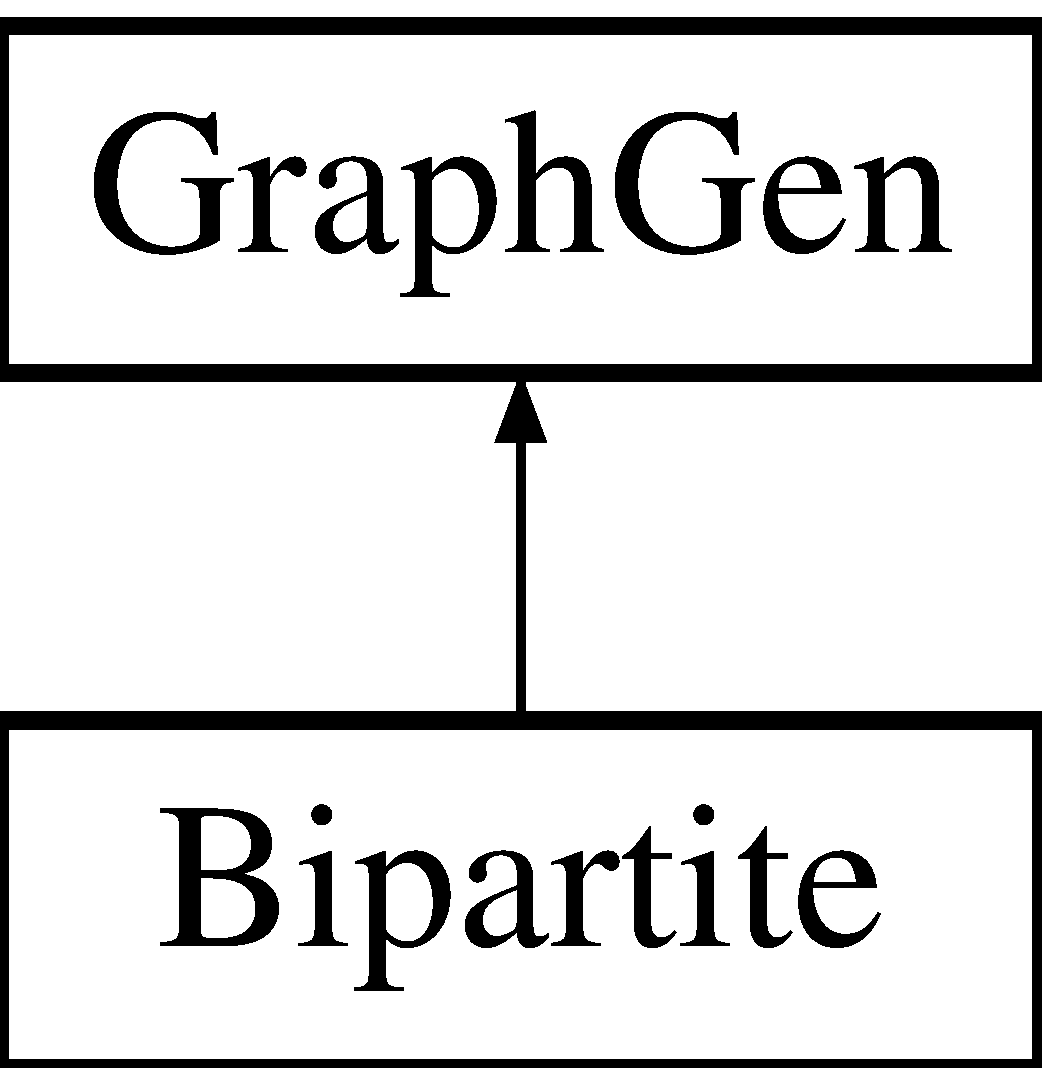
\includegraphics[height=2.000000cm]{classBipartite}
\end{center}
\end{figure}
\doxysubsection*{Membros públicos}
\begin{DoxyCompactItemize}
\item 
\mbox{\Hypertarget{classBipartite_aebea5d6981f517fa57e073c7d5cd5fd5}\label{classBipartite_aebea5d6981f517fa57e073c7d5cd5fd5}} 
\mbox{\hyperlink{classBipartite_aebea5d6981f517fa57e073c7d5cd5fd5}{Bipartite}} ()
\begin{DoxyCompactList}\small\item\em Construtor para o grafo bipartido vazio. \end{DoxyCompactList}\item 
\mbox{\Hypertarget{classBipartite_a1dfec46c393c2c1b8141250d26968673}\label{classBipartite_a1dfec46c393c2c1b8141250d26968673}} 
\mbox{\hyperlink{classBipartite_a1dfec46c393c2c1b8141250d26968673}{Bipartite}} (int)
\begin{DoxyCompactList}\small\item\em Construtor para o grafo bipartido por número de vértices. \end{DoxyCompactList}\item 
\mbox{\Hypertarget{classBipartite_a5535fa6da516192c5ec964b37db63e55}\label{classBipartite_a5535fa6da516192c5ec964b37db63e55}} 
\mbox{\hyperlink{classBipartite_a5535fa6da516192c5ec964b37db63e55}{Bipartite}} (\mbox{\hyperlink{classGraphGen}{Graph\+Gen}} \&)
\begin{DoxyCompactList}\small\item\em Construtor para o grafo bipartido por \mbox{\hyperlink{classGraphGen}{Graph\+Gen}}. \end{DoxyCompactList}\end{DoxyCompactItemize}
\doxysubsection*{Outros membros herdados}


\doxysubsection{Descrição detalhada}
Classe para grafos bipartidos. 

A documentação para esta classe foi gerada a partir do seguinte ficheiro\+:\begin{DoxyCompactItemize}
\item 
include/models/graph/\mbox{\hyperlink{Bipartite_8hpp}{Bipartite.\+hpp}}\end{DoxyCompactItemize}

\hypertarget{classBipartiteConstructorException}{}\doxysection{Referência à classe Bipartite\+Constructor\+Exception}
\label{classBipartiteConstructorException}\index{BipartiteConstructorException@{BipartiteConstructorException}}


Classe de exceções de construção de grafos bipartidos.  




{\ttfamily \#include $<$Bipartite.\+hpp$>$}

Diagrama de heranças da classe Bipartite\+Constructor\+Exception\begin{figure}[H]
\begin{center}
\leavevmode
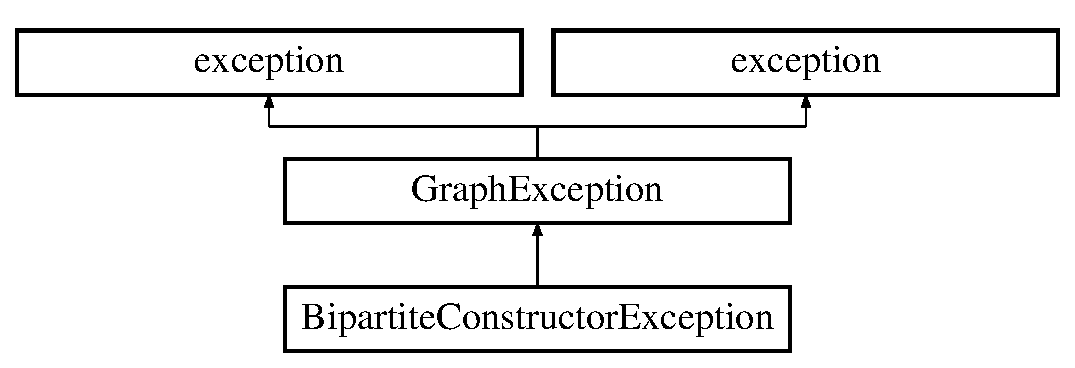
\includegraphics[height=3.000000cm]{classBipartiteConstructorException}
\end{center}
\end{figure}
\doxysubsection*{Membros públicos}
\begin{DoxyCompactItemize}
\item 
\mbox{\Hypertarget{classBipartiteConstructorException_a303013e25057612d9cac2e7450943d6d}\label{classBipartiteConstructorException_a303013e25057612d9cac2e7450943d6d}} 
\mbox{\hyperlink{classBipartiteConstructorException_a303013e25057612d9cac2e7450943d6d}{Bipartite\+Constructor\+Exception}} ()
\begin{DoxyCompactList}\small\item\em Construtor da exceção. \end{DoxyCompactList}\item 
\mbox{\Hypertarget{classBipartiteConstructorException_a11f033387020957b5ccd952914475807}\label{classBipartiteConstructorException_a11f033387020957b5ccd952914475807}} 
const char $\ast$ \mbox{\hyperlink{classBipartiteConstructorException_a11f033387020957b5ccd952914475807}{what}} () const  throw ()
\begin{DoxyCompactList}\small\item\em Retorna a mensagem de erro da exceção. \end{DoxyCompactList}\end{DoxyCompactItemize}


\doxysubsection{Descrição detalhada}
Classe de exceções de construção de grafos bipartidos. 

A documentação para esta classe foi gerada a partir do seguinte ficheiro\+:\begin{DoxyCompactItemize}
\item 
include/models/graph/\mbox{\hyperlink{Bipartite_8hpp}{Bipartite.\+hpp}}\end{DoxyCompactItemize}

\hypertarget{classChordal}{}\doxysection{Referência à classe Chordal}
\label{classChordal}\index{Chordal@{Chordal}}
Diagrama de heranças da classe Chordal\begin{figure}[H]
\begin{center}
\leavevmode
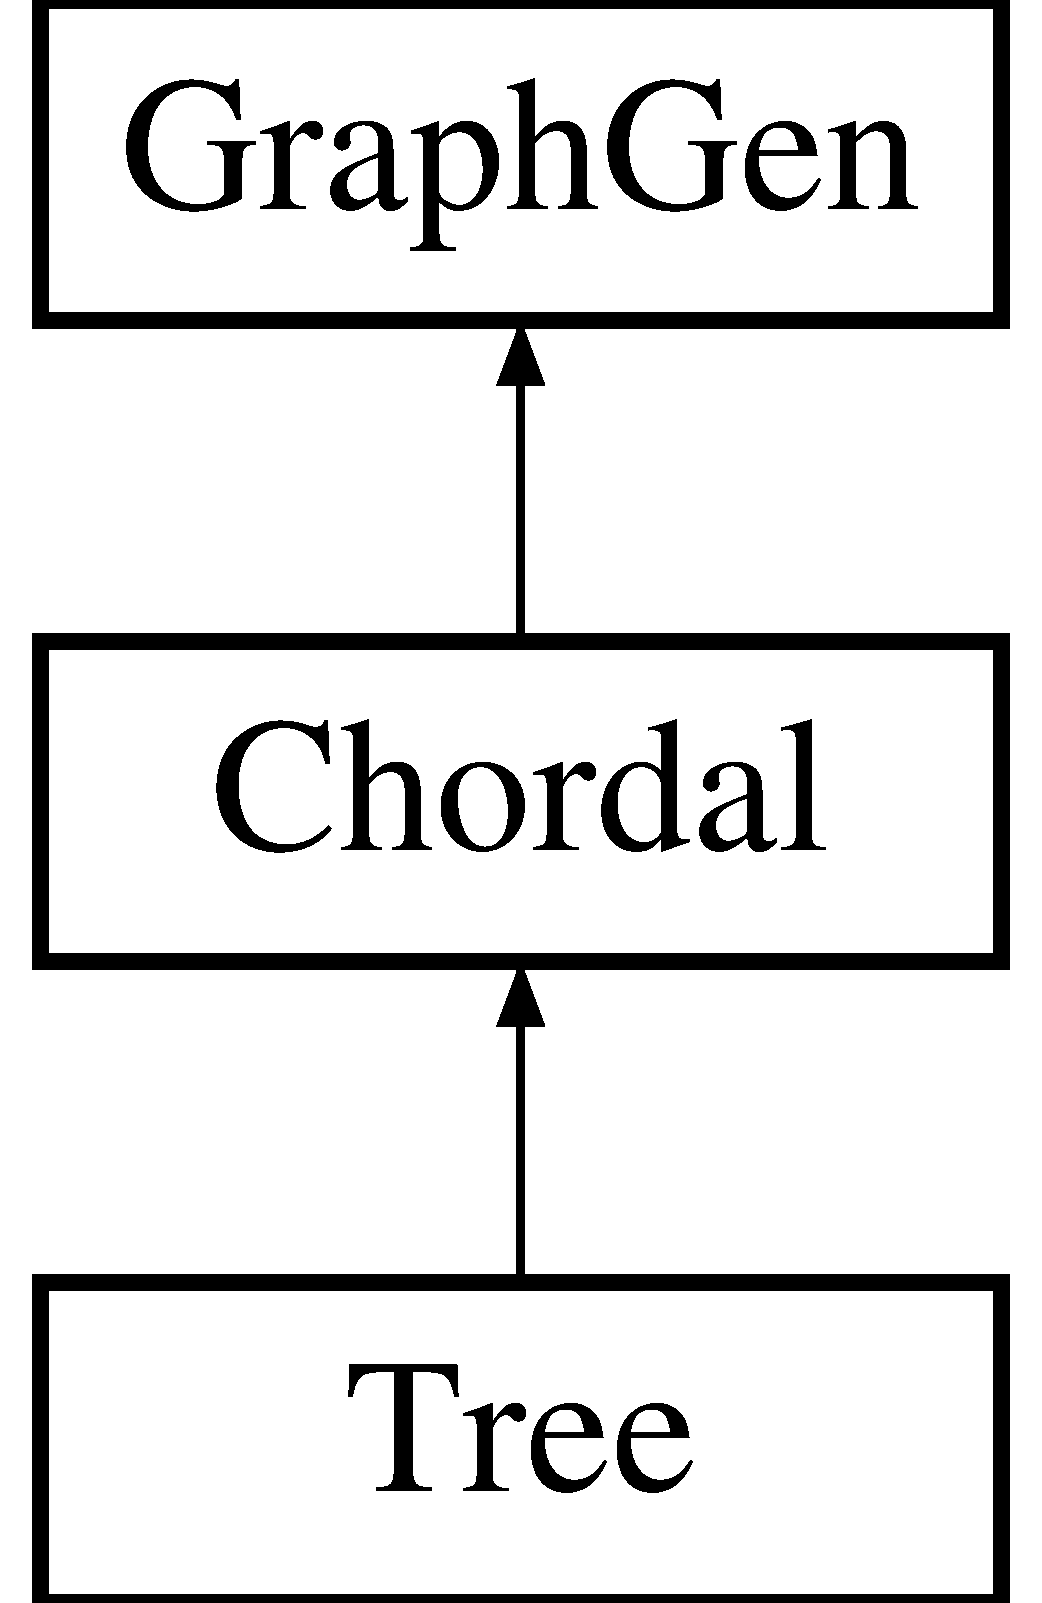
\includegraphics[height=2.000000cm]{classChordal}
\end{center}
\end{figure}
\doxysubsection*{Membros públicos}
\begin{DoxyCompactItemize}
\item 
\mbox{\Hypertarget{classChordal_af315e26462665f1881975cc27372a67a}\label{classChordal_af315e26462665f1881975cc27372a67a}} 
{\bfseries Chordal} (int)
\item 
\mbox{\Hypertarget{classChordal_a6ab51b523f1b150560fcae74db9eee68}\label{classChordal_a6ab51b523f1b150560fcae74db9eee68}} 
{\bfseries Chordal} (\mbox{\hyperlink{classGraphGen}{Graph\+Gen}} \&)
\item 
vector$<$ int $>$ \mbox{\hyperlink{classChordal_a45b66b1ee19a628646d83613d337d94a}{perfect\+Elimination\+Ordering}} ()
\item 
vector$<$ int $>$ \mbox{\hyperlink{classChordal_acac4822a1eb3376c29f3d193baaec91f}{coloring}} () override
\item 
int \mbox{\hyperlink{classChordal_ad7e9a3c8bd7f66ad4ddc6221523e6b12}{chromatic\+Number}} ()
\item 
int \mbox{\hyperlink{classChordal_aa19bddaef6b83d8bdb98993cf04929b7}{max\+Clique}} ()
\end{DoxyCompactItemize}
\doxysubsection*{Outros membros herdados}


\doxysubsection{Documentação dos métodos}
\mbox{\Hypertarget{classChordal_ad7e9a3c8bd7f66ad4ddc6221523e6b12}\label{classChordal_ad7e9a3c8bd7f66ad4ddc6221523e6b12}} 
\index{Chordal@{Chordal}!chromaticNumber@{chromaticNumber}}
\index{chromaticNumber@{chromaticNumber}!Chordal@{Chordal}}
\doxysubsubsection{\texorpdfstring{chromaticNumber()}{chromaticNumber()}}
{\footnotesize\ttfamily int Chordal\+::chromatic\+Number (\begin{DoxyParamCaption}{ }\end{DoxyParamCaption})}

Calcula o número cromático do grafo Complexidade\+: O(nlog() + m) \mbox{\Hypertarget{classChordal_acac4822a1eb3376c29f3d193baaec91f}\label{classChordal_acac4822a1eb3376c29f3d193baaec91f}} 
\index{Chordal@{Chordal}!coloring@{coloring}}
\index{coloring@{coloring}!Chordal@{Chordal}}
\doxysubsubsection{\texorpdfstring{coloring()}{coloring()}}
{\footnotesize\ttfamily vector$<$int$>$ Chordal\+::coloring (\begin{DoxyParamCaption}{ }\end{DoxyParamCaption})\hspace{0.3cm}{\ttfamily [override]}, {\ttfamily [virtual]}}

Algoritmo de coloração para grafos cordais. Complexidade\+: O(nlog() + m) 

Reimplementado de \mbox{\hyperlink{classGraphGen_ad44c80646f694460fafa3e3657beb4d0}{Graph\+Gen}}.

\mbox{\Hypertarget{classChordal_aa19bddaef6b83d8bdb98993cf04929b7}\label{classChordal_aa19bddaef6b83d8bdb98993cf04929b7}} 
\index{Chordal@{Chordal}!maxClique@{maxClique}}
\index{maxClique@{maxClique}!Chordal@{Chordal}}
\doxysubsubsection{\texorpdfstring{maxClique()}{maxClique()}}
{\footnotesize\ttfamily int Chordal\+::max\+Clique (\begin{DoxyParamCaption}{ }\end{DoxyParamCaption})}

Calcula o tamanho da maior clique do grafo Complexidade\+: O(nlog() + m) \mbox{\Hypertarget{classChordal_a45b66b1ee19a628646d83613d337d94a}\label{classChordal_a45b66b1ee19a628646d83613d337d94a}} 
\index{Chordal@{Chordal}!perfectEliminationOrdering@{perfectEliminationOrdering}}
\index{perfectEliminationOrdering@{perfectEliminationOrdering}!Chordal@{Chordal}}
\doxysubsubsection{\texorpdfstring{perfectEliminationOrdering()}{perfectEliminationOrdering()}}
{\footnotesize\ttfamily vector$<$int$>$ Chordal\+::perfect\+Elimination\+Ordering (\begin{DoxyParamCaption}{ }\end{DoxyParamCaption})}

Cria uma ordem de eliminação perfeita dos vértices. Complexidade\+: O(nlog(n)) 

A documentação para esta classe foi gerada a partir do seguinte ficheiro\+:\begin{DoxyCompactItemize}
\item 
include/models/graph/\mbox{\hyperlink{Chordal_8hpp}{Chordal.\+hpp}}\end{DoxyCompactItemize}

\hypertarget{classChordalConstructorException}{}\doxysection{Referência à classe Chordal\+Constructor\+Exception}
\label{classChordalConstructorException}\index{ChordalConstructorException@{ChordalConstructorException}}


Classe de exceções de construção de grafos cordais.  




{\ttfamily \#include $<$Chordal.\+hpp$>$}

Diagrama de heranças da classe Chordal\+Constructor\+Exception\begin{figure}[H]
\begin{center}
\leavevmode
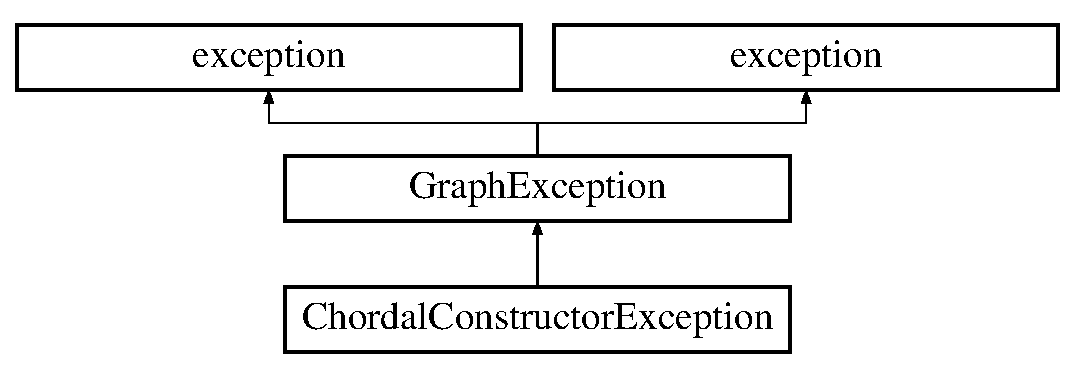
\includegraphics[height=3.000000cm]{classChordalConstructorException}
\end{center}
\end{figure}
\doxysubsection*{Membros públicos}
\begin{DoxyCompactItemize}
\item 
\mbox{\Hypertarget{classChordalConstructorException_a7b884c1b0146128227fc27162f2820c5}\label{classChordalConstructorException_a7b884c1b0146128227fc27162f2820c5}} 
\mbox{\hyperlink{classChordalConstructorException_a7b884c1b0146128227fc27162f2820c5}{Chordal\+Constructor\+Exception}} ()
\begin{DoxyCompactList}\small\item\em Construtor da exceção. \end{DoxyCompactList}\item 
\mbox{\Hypertarget{classChordalConstructorException_af45168f68f01e0b7cd98d8e82306a49b}\label{classChordalConstructorException_af45168f68f01e0b7cd98d8e82306a49b}} 
const char $\ast$ \mbox{\hyperlink{classChordalConstructorException_af45168f68f01e0b7cd98d8e82306a49b}{what}} () const  throw ()
\begin{DoxyCompactList}\small\item\em Retorna a mensagem de erro da exceção. \end{DoxyCompactList}\end{DoxyCompactItemize}


\doxysubsection{Descrição detalhada}
Classe de exceções de construção de grafos cordais. 

A documentação para esta classe foi gerada a partir do seguinte ficheiro\+:\begin{DoxyCompactItemize}
\item 
include/models/graph/\mbox{\hyperlink{Chordal_8hpp}{Chordal.\+hpp}}\end{DoxyCompactItemize}

\hypertarget{classDag}{}\section{Referência à classe Dag}
\label{classDag}\index{Dag@{Dag}}


Classe para grafos direcionados acíclicos.  




{\ttfamily \#include $<$Dag.\+hpp$>$}

Diagrama de heranças da classe Dag\begin{figure}[H]
\begin{center}
\leavevmode
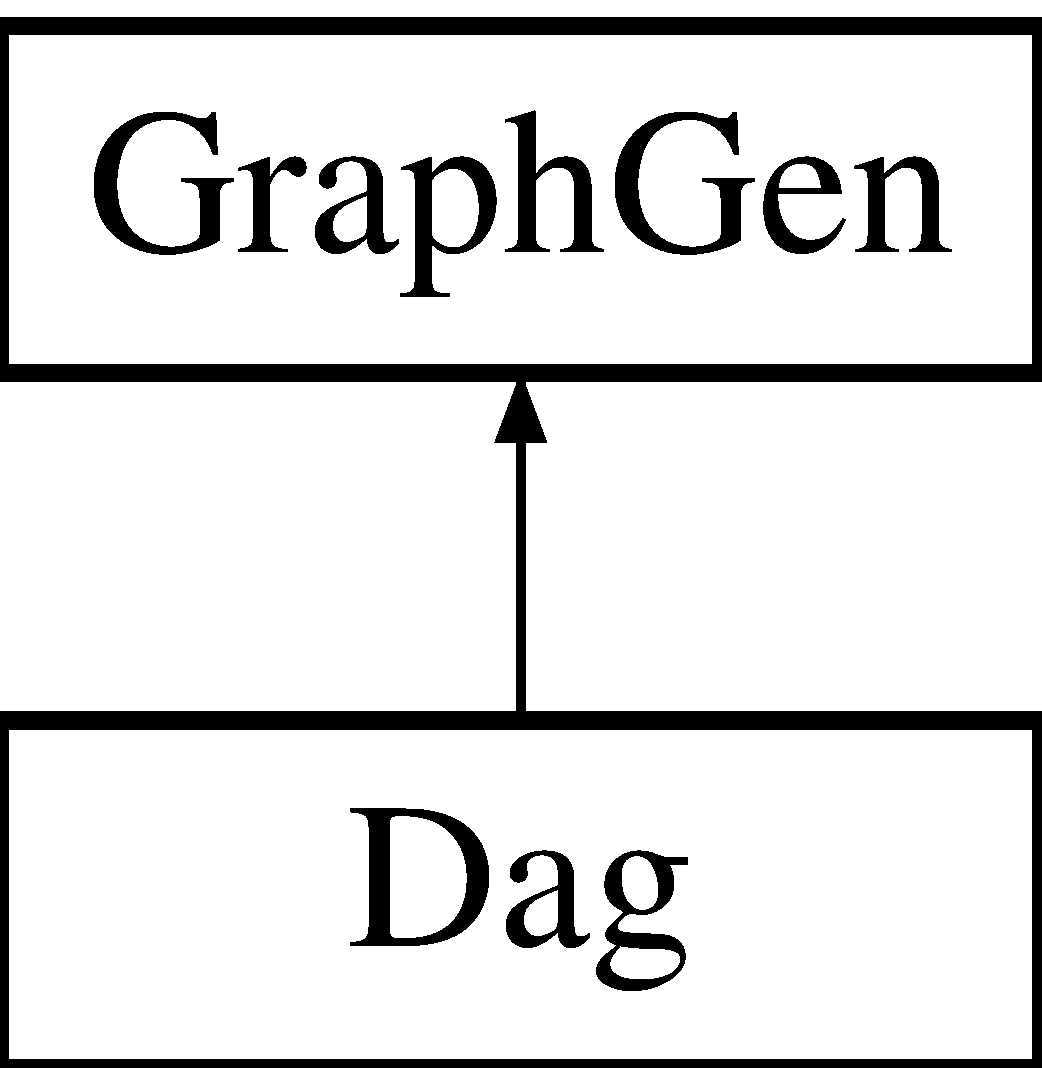
\includegraphics[height=2.000000cm]{classDag}
\end{center}
\end{figure}
\subsection*{Membros públicos}
\begin{DoxyCompactItemize}
\item 
\mbox{\Hypertarget{classDag_a9389de85348f50a4cad1681d5d573e12}\label{classDag_a9389de85348f50a4cad1681d5d573e12}} 
\hyperlink{classDag_a9389de85348f50a4cad1681d5d573e12}{Dag} ()
\begin{DoxyCompactList}\small\item\em Construtor de D\+A\+Gs vazios. \end{DoxyCompactList}\item 
\hyperlink{classDag_a60039050421d45ed24d5fff16dd0b4d9}{Dag} (int)
\item 
\hyperlink{classDag_a7ac03b3c8b13d4a85956eec57a1b8cd3}{Dag} (\hyperlink{classGraphGen}{Graph\+Gen} \&)
\item 
vector$<$ int $>$ \hyperlink{classDag_ac2f36e91443cfeea16640a81865110d2}{topo\+Sort} ()
\end{DoxyCompactItemize}
\subsection*{Outros membros herdados}


\subsection{Descrição detalhada}
Classe para grafos direcionados acíclicos. 

\subsection{Documentação dos Construtores \& Destrutor}
\mbox{\Hypertarget{classDag_a60039050421d45ed24d5fff16dd0b4d9}\label{classDag_a60039050421d45ed24d5fff16dd0b4d9}} 
\index{Dag@{Dag}!Dag@{Dag}}
\index{Dag@{Dag}!Dag@{Dag}}
\subsubsection{\texorpdfstring{Dag()}{Dag()}\hspace{0.1cm}{\footnotesize\ttfamily [1/2]}}
{\footnotesize\ttfamily Dag\+::\+Dag (\begin{DoxyParamCaption}\item[{int}]{ }\end{DoxyParamCaption})}

Construtor de D\+A\+Gs por número de vértices. 
\begin{DoxyParams}{Parâmetros}
{\em Número} & de vértices. \\
\hline
\end{DoxyParams}
\mbox{\Hypertarget{classDag_a7ac03b3c8b13d4a85956eec57a1b8cd3}\label{classDag_a7ac03b3c8b13d4a85956eec57a1b8cd3}} 
\index{Dag@{Dag}!Dag@{Dag}}
\index{Dag@{Dag}!Dag@{Dag}}
\subsubsection{\texorpdfstring{Dag()}{Dag()}\hspace{0.1cm}{\footnotesize\ttfamily [2/2]}}
{\footnotesize\ttfamily Dag\+::\+Dag (\begin{DoxyParamCaption}\item[{\hyperlink{classGraphGen}{Graph\+Gen} \&}]{ }\end{DoxyParamCaption})}

Construtor de D\+A\+Gs por por \hyperlink{classGraphGen}{Graph\+Gen}. 
\begin{DoxyParams}{Parâmetros}
{\em Grafo} & a ser convertido em D\+AG. \\
\hline
\end{DoxyParams}


\subsection{Documentação dos métodos}
\mbox{\Hypertarget{classDag_ac2f36e91443cfeea16640a81865110d2}\label{classDag_ac2f36e91443cfeea16640a81865110d2}} 
\index{Dag@{Dag}!topo\+Sort@{topo\+Sort}}
\index{topo\+Sort@{topo\+Sort}!Dag@{Dag}}
\subsubsection{\texorpdfstring{topo\+Sort()}{topoSort()}}
{\footnotesize\ttfamily vector$<$int$>$ Dag\+::topo\+Sort (\begin{DoxyParamCaption}{ }\end{DoxyParamCaption})}

Computa ordenação topológica. \begin{DoxyReturn}{Retorna}
Ordenação topológica dos vértices. 
\end{DoxyReturn}


A documentação para esta classe foi gerada a partir do seguinte ficheiro\+:\begin{DoxyCompactItemize}
\item 
include/models/graph/\hyperlink{Dag_8hpp}{Dag.\+hpp}\end{DoxyCompactItemize}

\hypertarget{classDagConstructorException}{}\doxysection{Referência à classe Dag\+Constructor\+Exception}
\label{classDagConstructorException}\index{DagConstructorException@{DagConstructorException}}


Classe de exceção de construção de D\+A\+Gs.  




{\ttfamily \#include $<$Dag.\+hpp$>$}

Diagrama de heranças da classe Dag\+Constructor\+Exception\begin{figure}[H]
\begin{center}
\leavevmode
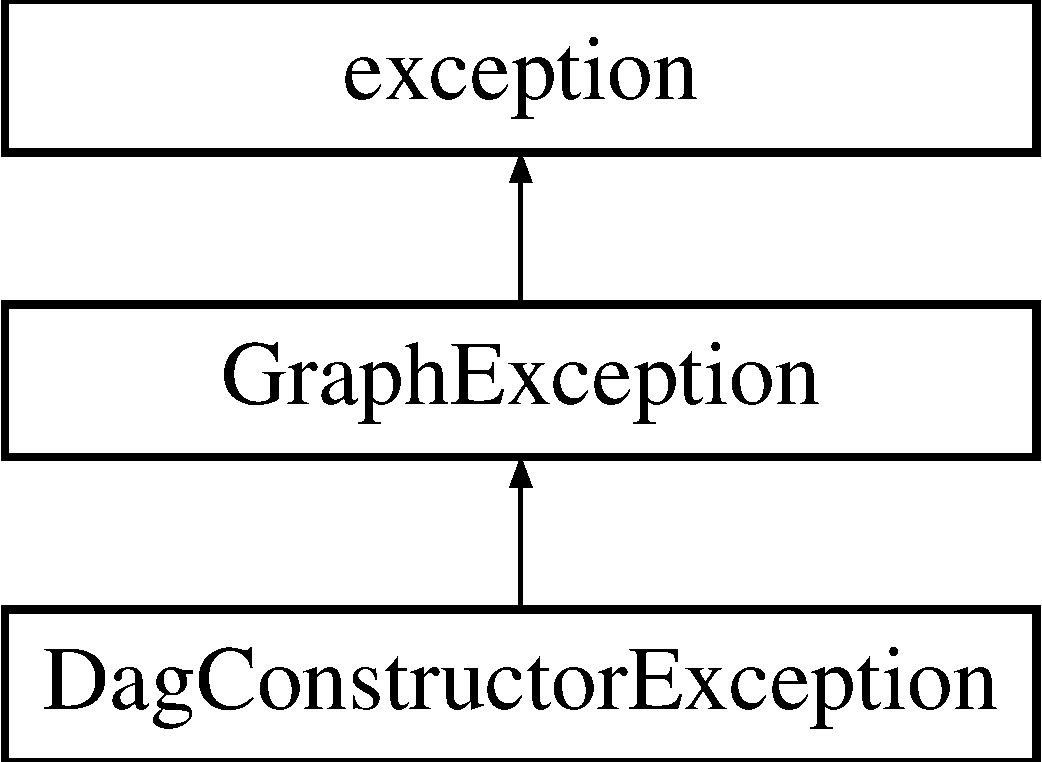
\includegraphics[height=3.000000cm]{classDagConstructorException}
\end{center}
\end{figure}
\doxysubsection*{Membros públicos}
\begin{DoxyCompactItemize}
\item 
\mbox{\Hypertarget{classDagConstructorException_a0c6e8ae8788ed7b42f73f4f1bfb0198f}\label{classDagConstructorException_a0c6e8ae8788ed7b42f73f4f1bfb0198f}} 
\mbox{\hyperlink{classDagConstructorException_a0c6e8ae8788ed7b42f73f4f1bfb0198f}{Dag\+Constructor\+Exception}} ()
\begin{DoxyCompactList}\small\item\em Construtor da exceção. \end{DoxyCompactList}\item 
\mbox{\Hypertarget{classDagConstructorException_a3ad88177747ce6ef7273d1196258c7ba}\label{classDagConstructorException_a3ad88177747ce6ef7273d1196258c7ba}} 
const char $\ast$ \mbox{\hyperlink{classDagConstructorException_a3ad88177747ce6ef7273d1196258c7ba}{what}} () const  throw ()
\begin{DoxyCompactList}\small\item\em Retorna a mensagem de erro da exceção. \end{DoxyCompactList}\end{DoxyCompactItemize}


\doxysubsection{Descrição detalhada}
Classe de exceção de construção de D\+A\+Gs. 

A documentação para esta classe foi gerada a partir do seguinte ficheiro\+:\begin{DoxyCompactItemize}
\item 
include/models/graph/\mbox{\hyperlink{Dag_8hpp}{Dag.\+hpp}}\end{DoxyCompactItemize}

\hypertarget{classDSU}{}\doxysection{Referência à classe D\+SU}
\label{classDSU}\index{DSU@{DSU}}


Classe para Disjoint Set Union (\mbox{\hyperlink{classDSU}{D\+SU}}).  




{\ttfamily \#include $<$D\+S\+U.\+hpp$>$}

\doxysubsection*{Membros públicos}
\begin{DoxyCompactItemize}
\item 
\mbox{\Hypertarget{classDSU_a537ec9947d526dd1ac2acc3bfe1bf8b3}\label{classDSU_a537ec9947d526dd1ac2acc3bfe1bf8b3}} 
\mbox{\hyperlink{classDSU_a537ec9947d526dd1ac2acc3bfe1bf8b3}{D\+SU}} ()
\begin{DoxyCompactList}\small\item\em Construtor para \mbox{\hyperlink{classDSU}{D\+SU}} vazio. \end{DoxyCompactList}\item 
\mbox{\Hypertarget{classDSU_ab4ea0f237eac81455e80443b3c060b40}\label{classDSU_ab4ea0f237eac81455e80443b3c060b40}} 
\mbox{\hyperlink{classDSU_ab4ea0f237eac81455e80443b3c060b40}{D\+SU}} (int)
\begin{DoxyCompactList}\small\item\em Construtor para \mbox{\hyperlink{classDSU}{D\+SU}} pelo número de elementos. \end{DoxyCompactList}\item 
int \mbox{\hyperlink{classDSU_a3915dd627bd9cd0abc6f83e154944961}{find}} (int)
\item 
void \mbox{\hyperlink{classDSU_a69728d8ed8c2262f76320ca7238e2f1f}{une}} (int, int)
\end{DoxyCompactItemize}


\doxysubsection{Descrição detalhada}
Classe para Disjoint Set Union (\mbox{\hyperlink{classDSU}{D\+SU}}). 

\doxysubsection{Documentação dos métodos}
\mbox{\Hypertarget{classDSU_a3915dd627bd9cd0abc6f83e154944961}\label{classDSU_a3915dd627bd9cd0abc6f83e154944961}} 
\index{DSU@{DSU}!find@{find}}
\index{find@{find}!DSU@{DSU}}
\doxysubsubsection{\texorpdfstring{find()}{find()}}
{\footnotesize\ttfamily int D\+S\+U\+::find (\begin{DoxyParamCaption}\item[{int}]{ }\end{DoxyParamCaption})}

Encontra representante do conjunto ao qual um elemento pretence.

Complexidade\+: O(inv\+Ackermann(n)) \mbox{\Hypertarget{classDSU_a69728d8ed8c2262f76320ca7238e2f1f}\label{classDSU_a69728d8ed8c2262f76320ca7238e2f1f}} 
\index{DSU@{DSU}!une@{une}}
\index{une@{une}!DSU@{DSU}}
\doxysubsubsection{\texorpdfstring{une()}{une()}}
{\footnotesize\ttfamily void D\+S\+U\+::une (\begin{DoxyParamCaption}\item[{int}]{,  }\item[{int}]{ }\end{DoxyParamCaption})}

Une dois conjuntos a partir de elementos dos mesmos.

Complexidade\+: O(inv\+Ackermann(n)) 

A documentação para esta classe foi gerada a partir do seguinte ficheiro\+:\begin{DoxyCompactItemize}
\item 
include/models/data\+Structures/\mbox{\hyperlink{DSU_8hpp}{D\+S\+U.\+hpp}}\end{DoxyCompactItemize}

\hypertarget{classDSUException}{}\doxysection{Referência à classe D\+S\+U\+Exception}
\label{classDSUException}\index{DSUException@{DSUException}}
Diagrama de heranças da classe D\+S\+U\+Exception\begin{figure}[H]
\begin{center}
\leavevmode
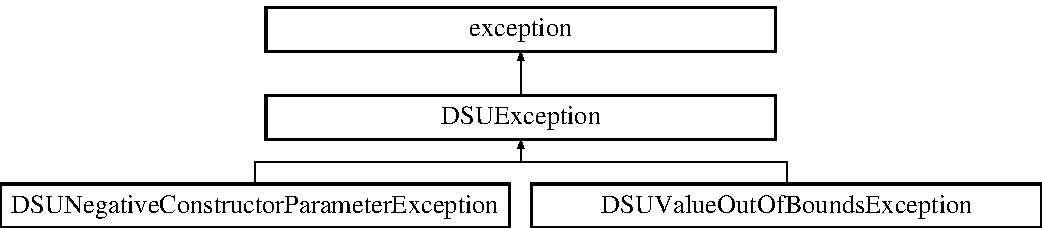
\includegraphics[height=3.000000cm]{classDSUException}
\end{center}
\end{figure}
\doxysubsection*{Membros públicos}
\begin{DoxyCompactItemize}
\item 
\mbox{\Hypertarget{classDSUException_a997fa79b5a7cd55cc30792da2303ea3a}\label{classDSUException_a997fa79b5a7cd55cc30792da2303ea3a}} 
const char $\ast$ {\bfseries what} () const  throw ()
\end{DoxyCompactItemize}


A documentação para esta classe foi gerada a partir do seguinte ficheiro\+:\begin{DoxyCompactItemize}
\item 
include/models/data\+Structures/D\+S\+U.\+hpp\end{DoxyCompactItemize}

\hypertarget{classDSUNegativeConstructorParameterException}{}\doxysection{Referência à classe D\+S\+U\+Negative\+Constructor\+Parameter\+Exception}
\label{classDSUNegativeConstructorParameterException}\index{DSUNegativeConstructorParameterException@{DSUNegativeConstructorParameterException}}


Classe de exceções de parâmetro negativo no construtor.  




{\ttfamily \#include $<$D\+S\+U.\+hpp$>$}

Diagrama de heranças da classe D\+S\+U\+Negative\+Constructor\+Parameter\+Exception\begin{figure}[H]
\begin{center}
\leavevmode
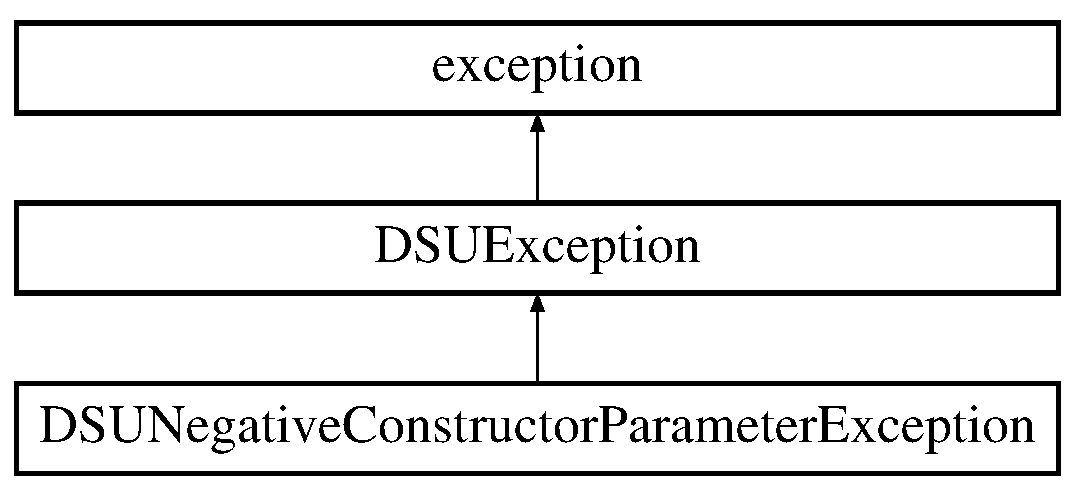
\includegraphics[height=3.000000cm]{classDSUNegativeConstructorParameterException}
\end{center}
\end{figure}
\doxysubsection*{Membros públicos}
\begin{DoxyCompactItemize}
\item 
\mbox{\Hypertarget{classDSUNegativeConstructorParameterException_a4d71581d8012d2d39ded7b6e240bc7e5}\label{classDSUNegativeConstructorParameterException_a4d71581d8012d2d39ded7b6e240bc7e5}} 
\mbox{\hyperlink{classDSUNegativeConstructorParameterException_a4d71581d8012d2d39ded7b6e240bc7e5}{D\+S\+U\+Negative\+Constructor\+Parameter\+Exception}} (int n)
\begin{DoxyCompactList}\small\item\em Construtor para exceção de parâmetro negativo. \end{DoxyCompactList}\item 
\mbox{\Hypertarget{classDSUNegativeConstructorParameterException_a16a3dcf8c0aeca0c1158ee18dd2a0c0f}\label{classDSUNegativeConstructorParameterException_a16a3dcf8c0aeca0c1158ee18dd2a0c0f}} 
const char $\ast$ \mbox{\hyperlink{classDSUNegativeConstructorParameterException_a16a3dcf8c0aeca0c1158ee18dd2a0c0f}{what}} () const  throw ()
\begin{DoxyCompactList}\small\item\em Retorna a mensagem de erro da exceção. \end{DoxyCompactList}\end{DoxyCompactItemize}


\doxysubsection{Descrição detalhada}
Classe de exceções de parâmetro negativo no construtor. 

A documentação para esta classe foi gerada a partir do seguinte ficheiro\+:\begin{DoxyCompactItemize}
\item 
include/models/data\+Structures/\mbox{\hyperlink{DSU_8hpp}{D\+S\+U.\+hpp}}\end{DoxyCompactItemize}

\hypertarget{classDSUValueOutOfBoundsException}{}\doxysection{Referência à classe D\+S\+U\+Value\+Out\+Of\+Bounds\+Exception}
\label{classDSUValueOutOfBoundsException}\index{DSUValueOutOfBoundsException@{DSUValueOutOfBoundsException}}
Diagrama de heranças da classe D\+S\+U\+Value\+Out\+Of\+Bounds\+Exception\begin{figure}[H]
\begin{center}
\leavevmode
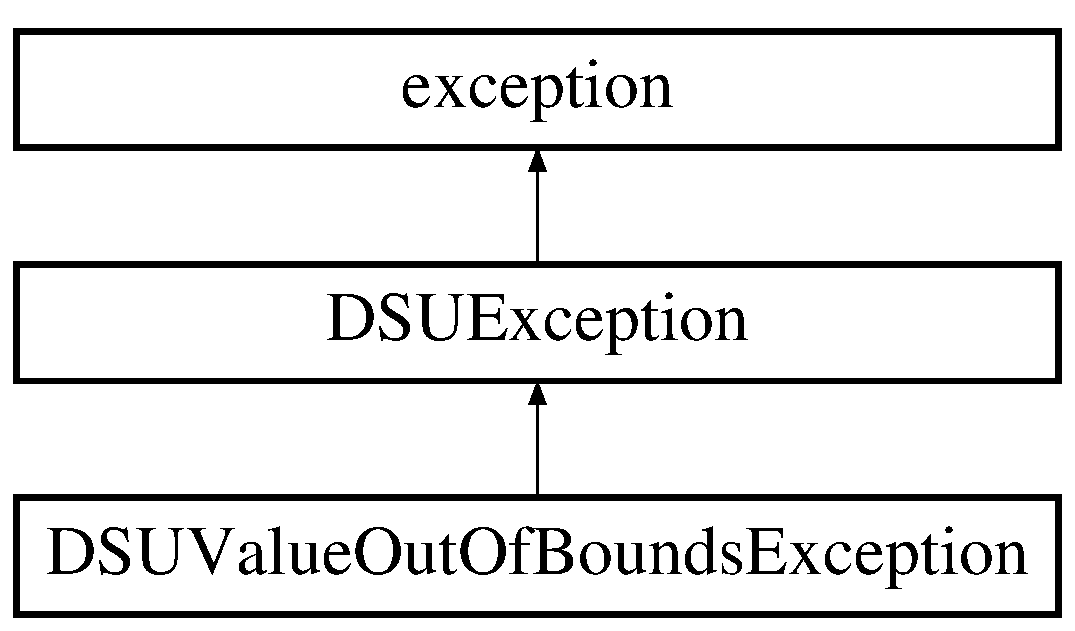
\includegraphics[height=3.000000cm]{classDSUValueOutOfBoundsException}
\end{center}
\end{figure}
\doxysubsection*{Membros públicos}
\begin{DoxyCompactItemize}
\item 
\mbox{\Hypertarget{classDSUValueOutOfBoundsException_ace15ec35fac30116b21fe713f59f2943}\label{classDSUValueOutOfBoundsException_ace15ec35fac30116b21fe713f59f2943}} 
{\bfseries D\+S\+U\+Value\+Out\+Of\+Bounds\+Exception} (int n)
\item 
\mbox{\Hypertarget{classDSUValueOutOfBoundsException_a20697d2be588c4f19046c9f468675bde}\label{classDSUValueOutOfBoundsException_a20697d2be588c4f19046c9f468675bde}} 
const char $\ast$ {\bfseries what} () const  throw ()
\end{DoxyCompactItemize}


A documentação para esta classe foi gerada a partir do seguinte ficheiro\+:\begin{DoxyCompactItemize}
\item 
include/models/data\+Structures/D\+S\+U.\+hpp\end{DoxyCompactItemize}

\hypertarget{classFileNotFoundException}{}\section{Referência à classe File\+Not\+Found\+Exception}
\label{classFileNotFoundException}\index{File\+Not\+Found\+Exception@{File\+Not\+Found\+Exception}}


Classe de exceções para leitura de grafos inexistentes.  




{\ttfamily \#include $<$Graph\+Canvas.\+hpp$>$}

Diagrama de heranças da classe File\+Not\+Found\+Exception\begin{figure}[H]
\begin{center}
\leavevmode
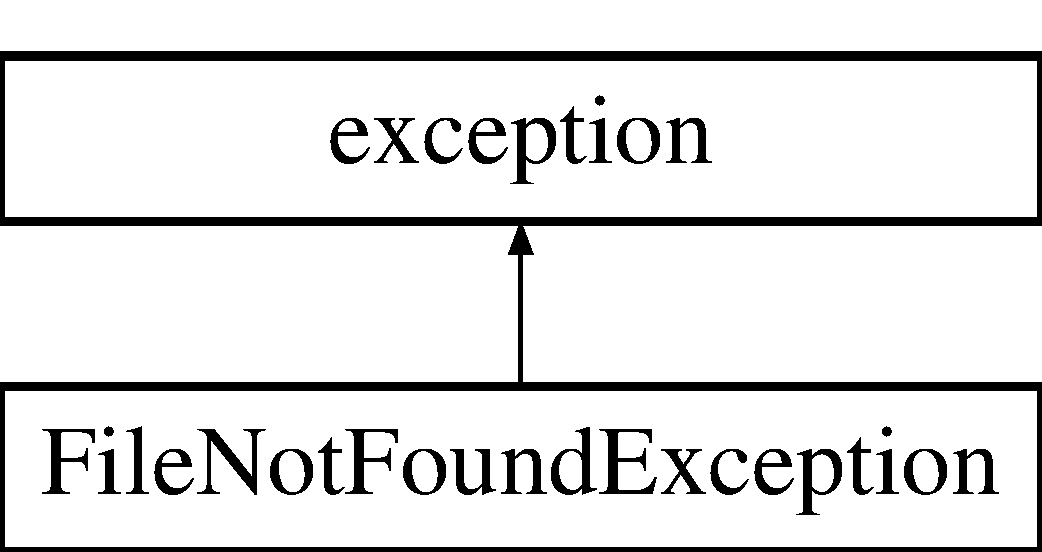
\includegraphics[height=2.000000cm]{classFileNotFoundException}
\end{center}
\end{figure}
\subsection*{Membros públicos}
\begin{DoxyCompactItemize}
\item 
\hyperlink{classFileNotFoundException_a9d496f2fcb769c4ae3f2ba1bd5c4840c}{File\+Not\+Found\+Exception} (string f)
\item 
const char $\ast$ \hyperlink{classFileNotFoundException_a7b845599455543d92dffe50950f5fa8d}{what} () const  throw ()
\end{DoxyCompactItemize}


\subsection{Descrição detalhada}
Classe de exceções para leitura de grafos inexistentes. 

\subsection{Documentação dos Construtores \& Destrutor}
\mbox{\Hypertarget{classFileNotFoundException_a9d496f2fcb769c4ae3f2ba1bd5c4840c}\label{classFileNotFoundException_a9d496f2fcb769c4ae3f2ba1bd5c4840c}} 
\index{File\+Not\+Found\+Exception@{File\+Not\+Found\+Exception}!File\+Not\+Found\+Exception@{File\+Not\+Found\+Exception}}
\index{File\+Not\+Found\+Exception@{File\+Not\+Found\+Exception}!File\+Not\+Found\+Exception@{File\+Not\+Found\+Exception}}
\subsubsection{\texorpdfstring{File\+Not\+Found\+Exception()}{FileNotFoundException()}}
{\footnotesize\ttfamily File\+Not\+Found\+Exception\+::\+File\+Not\+Found\+Exception (\begin{DoxyParamCaption}\item[{string}]{f }\end{DoxyParamCaption})\hspace{0.3cm}{\ttfamily [inline]}}

Construtor da exceção. 
\begin{DoxyParams}{Parâmetros}
{\em Nome} & do arquivo. \\
\hline
\end{DoxyParams}


\subsection{Documentação dos métodos}
\mbox{\Hypertarget{classFileNotFoundException_a7b845599455543d92dffe50950f5fa8d}\label{classFileNotFoundException_a7b845599455543d92dffe50950f5fa8d}} 
\index{File\+Not\+Found\+Exception@{File\+Not\+Found\+Exception}!what@{what}}
\index{what@{what}!File\+Not\+Found\+Exception@{File\+Not\+Found\+Exception}}
\subsubsection{\texorpdfstring{what()}{what()}}
{\footnotesize\ttfamily const char$\ast$ File\+Not\+Found\+Exception\+::what (\begin{DoxyParamCaption}{ }\end{DoxyParamCaption}) const throw  ) \hspace{0.3cm}{\ttfamily [inline]}}

Retorna a mensagem de erro da exceção. \begin{DoxyReturn}{Retorna}
Mensagem de erro. 
\end{DoxyReturn}


A documentação para esta classe foi gerada a partir do seguinte ficheiro\+:\begin{DoxyCompactItemize}
\item 
include/views/\hyperlink{GraphCanvas_8hpp}{Graph\+Canvas.\+hpp}\end{DoxyCompactItemize}

\hypertarget{classGraph}{}\doxysection{Referência à classe Graph}
\label{classGraph}\index{Graph@{Graph}}


Classe para grafos.  




{\ttfamily \#include $<$Graph.\+hpp$>$}

Diagrama de heranças da classe Graph\begin{figure}[H]
\begin{center}
\leavevmode
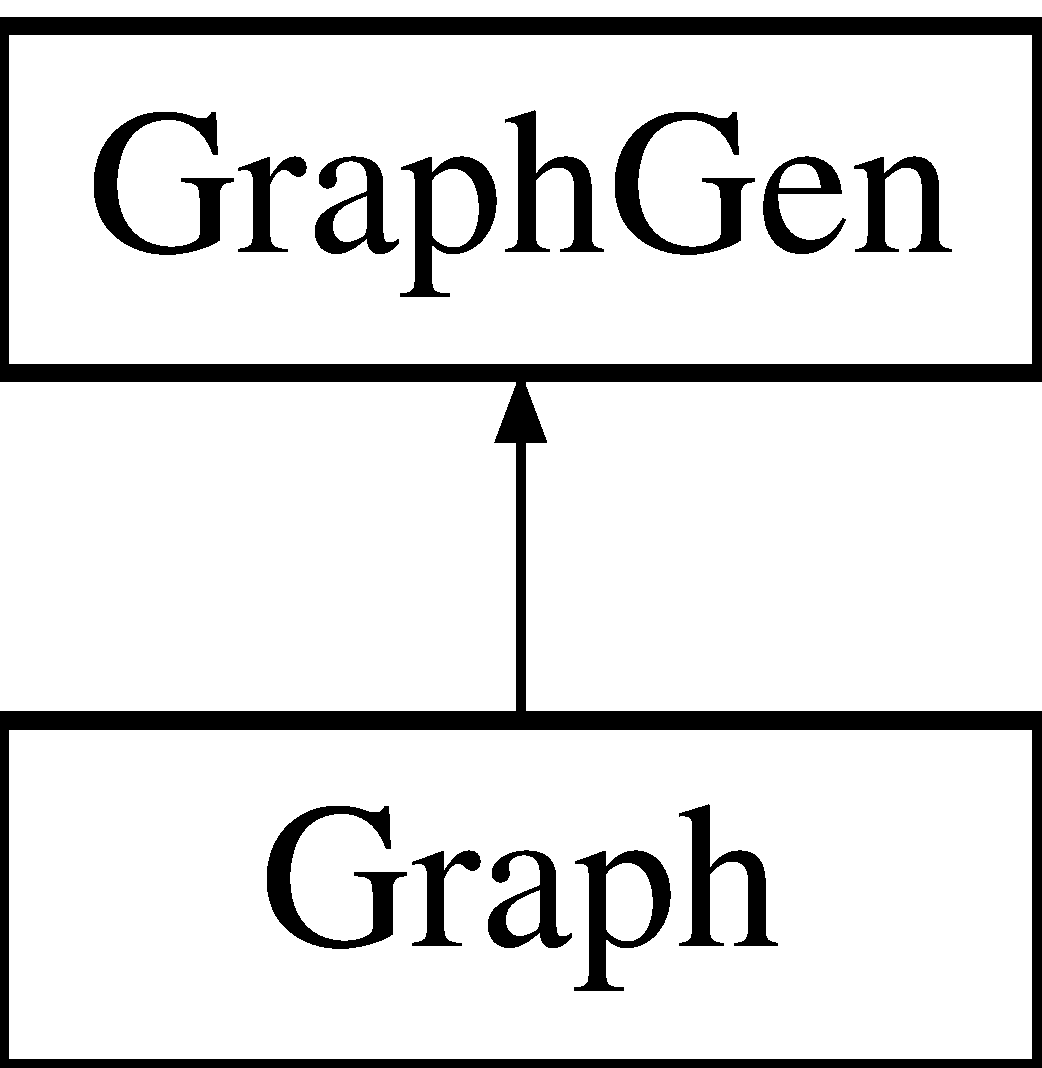
\includegraphics[height=2.000000cm]{classGraph}
\end{center}
\end{figure}
\doxysubsection*{Membros públicos}
\begin{DoxyCompactItemize}
\item 
\mbox{\Hypertarget{classGraph_ae4c72b8ac4d693c49800a4c7e273654f}\label{classGraph_ae4c72b8ac4d693c49800a4c7e273654f}} 
\mbox{\hyperlink{classGraph_ae4c72b8ac4d693c49800a4c7e273654f}{Graph}} ()
\begin{DoxyCompactList}\small\item\em Construtor do grafo. \end{DoxyCompactList}\item 
\mbox{\Hypertarget{classGraph_a6381663d9f8215c377123a3a8107011c}\label{classGraph_a6381663d9f8215c377123a3a8107011c}} 
\mbox{\hyperlink{classGraph_a6381663d9f8215c377123a3a8107011c}{Graph}} (int)
\begin{DoxyCompactList}\small\item\em Construtor do grafo por número de vértices. \end{DoxyCompactList}\item 
\mbox{\Hypertarget{classGraph_a0cb28a8601b14d0cb4291e5f60882ffc}\label{classGraph_a0cb28a8601b14d0cb4291e5f60882ffc}} 
\mbox{\hyperlink{classGraph_a0cb28a8601b14d0cb4291e5f60882ffc}{Graph}} (int, vector$<$ string $>$ \&)
\begin{DoxyCompactList}\small\item\em Construtor do grafo por número de vértices e seus rótulos. \end{DoxyCompactList}\item 
\mbox{\Hypertarget{classGraph_a0cd2695bebb326da026ed7391542aba6}\label{classGraph_a0cd2695bebb326da026ed7391542aba6}} 
\mbox{\hyperlink{classGraph_a0cd2695bebb326da026ed7391542aba6}{Graph}} (\mbox{\hyperlink{classGraphGen}{Graph\+Gen}} \&)
\begin{DoxyCompactList}\small\item\em Construtor do grafo por \mbox{\hyperlink{classGraphGen}{Graph\+Gen}}. \end{DoxyCompactList}\item 
\mbox{\Hypertarget{classGraph_a9f627b8aaa697daabe0ed31bbd0953eb}\label{classGraph_a9f627b8aaa697daabe0ed31bbd0953eb}} 
void \mbox{\hyperlink{classGraph_a9f627b8aaa697daabe0ed31bbd0953eb}{add\+Edge}} (int, int)
\begin{DoxyCompactList}\small\item\em Adiciona aresta sem peso entre dois vértices. \end{DoxyCompactList}\item 
\mbox{\Hypertarget{classGraph_ad4155b07ec70e1d85787710452a2bcfa}\label{classGraph_ad4155b07ec70e1d85787710452a2bcfa}} 
void \mbox{\hyperlink{classGraph_ad4155b07ec70e1d85787710452a2bcfa}{add\+Edge}} (int, int, int)
\begin{DoxyCompactList}\small\item\em Adiciona aresta com peso entre dois vértices. \end{DoxyCompactList}\item 
\mbox{\hyperlink{classTree}{Tree}} \mbox{\hyperlink{classGraph_a59f3bafa5e1935a2de4313b43219c4d6}{mst}} ()
\item 
vector$<$ bool $>$ \mbox{\hyperlink{classGraph_a645760818f3f2a20f8593b6b2a65c2d8}{mst\+Edges}} ()
\end{DoxyCompactItemize}
\doxysubsection*{Outros membros herdados}


\doxysubsection{Descrição detalhada}
Classe para grafos. 

\doxysubsection{Documentação dos métodos}
\mbox{\Hypertarget{classGraph_a59f3bafa5e1935a2de4313b43219c4d6}\label{classGraph_a59f3bafa5e1935a2de4313b43219c4d6}} 
\index{Graph@{Graph}!mst@{mst}}
\index{mst@{mst}!Graph@{Graph}}
\doxysubsubsection{\texorpdfstring{mst()}{mst()}}
{\footnotesize\ttfamily \mbox{\hyperlink{classTree}{Tree}} Graph\+::mst (\begin{DoxyParamCaption}{ }\end{DoxyParamCaption})}

Encontra uma árvore geradora mínima para o grafo.

Complexidade\+: O() \mbox{\Hypertarget{classGraph_a645760818f3f2a20f8593b6b2a65c2d8}\label{classGraph_a645760818f3f2a20f8593b6b2a65c2d8}} 
\index{Graph@{Graph}!mstEdges@{mstEdges}}
\index{mstEdges@{mstEdges}!Graph@{Graph}}
\doxysubsubsection{\texorpdfstring{mstEdges()}{mstEdges()}}
{\footnotesize\ttfamily vector$<$bool$>$ Graph\+::mst\+Edges (\begin{DoxyParamCaption}{ }\end{DoxyParamCaption})}

Retorna uma lista das arestas que pertencem a uma árvore geradora mínima.

Complexidade\+: O() 

A documentação para esta classe foi gerada a partir do seguinte ficheiro\+:\begin{DoxyCompactItemize}
\item 
include/models/graph/\mbox{\hyperlink{Graph_8hpp}{Graph.\+hpp}}\end{DoxyCompactItemize}

\hypertarget{classGraphCanvas}{}\section{Referência à classe Graph\+Canvas}
\label{classGraphCanvas}\index{Graph\+Canvas@{Graph\+Canvas}}


Classe para o canvas.  




{\ttfamily \#include $<$Graph\+Canvas.\+hpp$>$}

\subsection*{Membros públicos}
\begin{DoxyCompactItemize}
\item 
\mbox{\Hypertarget{classGraphCanvas_a0868eb47bb561e5037b24dc06fad52c7}\label{classGraphCanvas_a0868eb47bb561e5037b24dc06fad52c7}} 
\hyperlink{classGraphCanvas_a0868eb47bb561e5037b24dc06fad52c7}{Graph\+Canvas} ()
\begin{DoxyCompactList}\small\item\em Construtor vazio. \end{DoxyCompactList}\item 
\hyperlink{classGraphCanvas_a7852754f721735c6d8672673a50401cc}{Graph\+Canvas} (sf\+::\+Render\+Window \&, sf\+::\+Font \&, int, int, int)
\item 
void \hyperlink{classGraphCanvas_a1f402e85859d1eb3b6f1965de3def1af}{set\+Graph} (\hyperlink{classGraph}{Graph})
\item 
bool \hyperlink{classGraphCanvas_a4115aea20f2f1352b674ef9cfb6579a4}{handle\+Clique} ()
\item 
\mbox{\Hypertarget{classGraphCanvas_a236523bfec7a55f8ea70c09fdb3590c3}\label{classGraphCanvas_a236523bfec7a55f8ea70c09fdb3590c3}} 
void \hyperlink{classGraphCanvas_a236523bfec7a55f8ea70c09fdb3590c3}{display} ()
\begin{DoxyCompactList}\small\item\em Exibe o grafo. \end{DoxyCompactList}\end{DoxyCompactItemize}
\subsection*{Atributos Públicos}
\begin{DoxyCompactItemize}
\item 
\mbox{\Hypertarget{classGraphCanvas_a7e2f16ce3638db53fb73061fe1c93f15}\label{classGraphCanvas_a7e2f16ce3638db53fb73061fe1c93f15}} 
\hyperlink{classGraphDisplay}{Graph\+Display} \hyperlink{classGraphCanvas_a7e2f16ce3638db53fb73061fe1c93f15}{GD}
\begin{DoxyCompactList}\small\item\em Display do canvas. \end{DoxyCompactList}\item 
\mbox{\Hypertarget{classGraphCanvas_acbae5a92eb6cdc7cd7714093295f5412}\label{classGraphCanvas_acbae5a92eb6cdc7cd7714093295f5412}} 
sf\+::\+Render\+Window $\ast$ \hyperlink{classGraphCanvas_acbae5a92eb6cdc7cd7714093295f5412}{janela}
\begin{DoxyCompactList}\small\item\em Objeto Render\+Window para trabalhar no canvas. \end{DoxyCompactList}\item 
\mbox{\Hypertarget{classGraphCanvas_a74e79b17a3bbfa10dfa1bbe9f1aeb47d}\label{classGraphCanvas_a74e79b17a3bbfa10dfa1bbe9f1aeb47d}} 
sf\+::\+Font \hyperlink{classGraphCanvas_a74e79b17a3bbfa10dfa1bbe9f1aeb47d}{fonte}
\begin{DoxyCompactList}\small\item\em Fonte para textos da interface. \end{DoxyCompactList}\item 
\mbox{\Hypertarget{classGraphCanvas_a65406a215bd30e44358031c5b8a2cc2b}\label{classGraphCanvas_a65406a215bd30e44358031c5b8a2cc2b}} 
int \hyperlink{classGraphCanvas_a65406a215bd30e44358031c5b8a2cc2b}{edit\+Label}
\begin{DoxyCompactList}\small\item\em Vértice que o usuário está editando. \end{DoxyCompactList}\item 
\mbox{\Hypertarget{classGraphCanvas_a3b81b5c942b2fe3d94952d7ce664d3ed}\label{classGraphCanvas_a3b81b5c942b2fe3d94952d7ce664d3ed}} 
int \hyperlink{classGraphCanvas_a3b81b5c942b2fe3d94952d7ce664d3ed}{edit\+Weight}
\begin{DoxyCompactList}\small\item\em Aresta que o usuário está editando. \end{DoxyCompactList}\end{DoxyCompactItemize}


\subsection{Descrição detalhada}
Classe para o canvas. 

\subsection{Documentação dos Construtores \& Destrutor}
\mbox{\Hypertarget{classGraphCanvas_a7852754f721735c6d8672673a50401cc}\label{classGraphCanvas_a7852754f721735c6d8672673a50401cc}} 
\index{Graph\+Canvas@{Graph\+Canvas}!Graph\+Canvas@{Graph\+Canvas}}
\index{Graph\+Canvas@{Graph\+Canvas}!Graph\+Canvas@{Graph\+Canvas}}
\subsubsection{\texorpdfstring{Graph\+Canvas()}{GraphCanvas()}}
{\footnotesize\ttfamily Graph\+Canvas\+::\+Graph\+Canvas (\begin{DoxyParamCaption}\item[{sf\+::\+Render\+Window \&}]{,  }\item[{sf\+::\+Font \&}]{,  }\item[{int}]{,  }\item[{int}]{,  }\item[{int}]{ }\end{DoxyParamCaption})}

Construtor da classe. 
\begin{DoxyParams}{Parâmetros}
{\em Janela.} & \\
\hline
{\em Fonte.} & \\
\hline
{\em X} & e Y que delimitam o canvas. \\
\hline
{\em raio} & do vértice. \\
\hline
\end{DoxyParams}


\subsection{Documentação dos métodos}
\mbox{\Hypertarget{classGraphCanvas_a4115aea20f2f1352b674ef9cfb6579a4}\label{classGraphCanvas_a4115aea20f2f1352b674ef9cfb6579a4}} 
\index{Graph\+Canvas@{Graph\+Canvas}!handle\+Clique@{handle\+Clique}}
\index{handle\+Clique@{handle\+Clique}!Graph\+Canvas@{Graph\+Canvas}}
\subsubsection{\texorpdfstring{handle\+Clique()}{handleClique()}}
{\footnotesize\ttfamily bool Graph\+Canvas\+::handle\+Clique (\begin{DoxyParamCaption}{ }\end{DoxyParamCaption})}

Trata o clique do usuário, descobrindo se ele clicou num vértice, aresta, etc. \begin{DoxyReturn}{Retorna}
bool que informa se algo foi alterado no canvas. 
\end{DoxyReturn}
\mbox{\Hypertarget{classGraphCanvas_a1f402e85859d1eb3b6f1965de3def1af}\label{classGraphCanvas_a1f402e85859d1eb3b6f1965de3def1af}} 
\index{Graph\+Canvas@{Graph\+Canvas}!set\+Graph@{set\+Graph}}
\index{set\+Graph@{set\+Graph}!Graph\+Canvas@{Graph\+Canvas}}
\subsubsection{\texorpdfstring{set\+Graph()}{setGraph()}}
{\footnotesize\ttfamily void Graph\+Canvas\+::set\+Graph (\begin{DoxyParamCaption}\item[{\hyperlink{classGraph}{Graph}}]{ }\end{DoxyParamCaption})}

Define o grafo a ser representado. 
\begin{DoxyParams}{Parâmetros}
{\em Grafo} & a ser representado. \\
\hline
\end{DoxyParams}


A documentação para esta classe foi gerada a partir do seguinte ficheiro\+:\begin{DoxyCompactItemize}
\item 
include/views/\hyperlink{GraphCanvas_8hpp}{Graph\+Canvas.\+hpp}\end{DoxyCompactItemize}

\hypertarget{classGraphDisplay}{}\doxysection{Referência à classe Graph\+Display}
\label{classGraphDisplay}\index{GraphDisplay@{GraphDisplay}}


Classe para display do grafo.  




{\ttfamily \#include $<$Graph\+Display.\+hpp$>$}

\doxysubsection*{Membros públicos}
\begin{DoxyCompactItemize}
\item 
\mbox{\Hypertarget{classGraphDisplay_ac208e50545ccedbca810822743040f48}\label{classGraphDisplay_ac208e50545ccedbca810822743040f48}} 
\mbox{\hyperlink{classGraphDisplay_ac208e50545ccedbca810822743040f48}{Graph\+Display}} ()
\begin{DoxyCompactList}\small\item\em Construtor de \mbox{\hyperlink{classGraphDisplay}{Graph\+Display}} vazio. \end{DoxyCompactList}\item 
\mbox{\hyperlink{classGraphDisplay_adea7ab840d8aa0646eab49709569143f}{Graph\+Display}} (\mbox{\hyperlink{classGraph}{Graph}}, int, int, int)
\item 
\mbox{\Hypertarget{classGraphDisplay_a496ee74caea737ce5f93f9d23474eb6d}\label{classGraphDisplay_a496ee74caea737ce5f93f9d23474eb6d}} 
void \mbox{\hyperlink{classGraphDisplay_a496ee74caea737ce5f93f9d23474eb6d}{set\+Graph}} (\mbox{\hyperlink{classGraph}{Graph}} \&)
\begin{DoxyCompactList}\small\item\em Seta um grafo no display. \end{DoxyCompactList}\item 
\mbox{\Hypertarget{classGraphDisplay_ab90cdfe3694a8a34767dc50268cf5a50}\label{classGraphDisplay_ab90cdfe3694a8a34767dc50268cf5a50}} 
void \mbox{\hyperlink{classGraphDisplay_ab90cdfe3694a8a34767dc50268cf5a50}{set\+Graph\+Continue}} (\mbox{\hyperlink{classGraph}{Graph}} \&)
\begin{DoxyCompactList}\small\item\em Seta um grafo no display, mantendo as confugurações do grafo anterior. \end{DoxyCompactList}\item 
\mbox{\Hypertarget{classGraphDisplay_a9d55e916fea8b749eaee51def8d004d3}\label{classGraphDisplay_a9d55e916fea8b749eaee51def8d004d3}} 
void \mbox{\hyperlink{classGraphDisplay_a9d55e916fea8b749eaee51def8d004d3}{fdp\+Peso}} (int)
\begin{DoxyCompactList}\small\item\em Algoritmo de display para os pesos. \end{DoxyCompactList}\item 
\mbox{\Hypertarget{classGraphDisplay_a694d361743f700a6250d578978aefab1}\label{classGraphDisplay_a694d361743f700a6250d578978aefab1}} 
\mbox{\hyperlink{classVector}{Vector}} \mbox{\hyperlink{classGraphDisplay_a694d361743f700a6250d578978aefab1}{deixa\+Dentro}} (\mbox{\hyperlink{classVector}{Vector}}, bool)
\begin{DoxyCompactList}\small\item\em Garante que um vértice está dentro do canvas. \end{DoxyCompactList}\item 
\mbox{\Hypertarget{classGraphDisplay_a6d822244f05f8a0dd1e40a40d13294bf}\label{classGraphDisplay_a6d822244f05f8a0dd1e40a40d13294bf}} 
bool \mbox{\hyperlink{classGraphDisplay_a6d822244f05f8a0dd1e40a40d13294bf}{ta\+Dentro}} (\mbox{\hyperlink{classVector}{Vector}})
\begin{DoxyCompactList}\small\item\em Verifica se uma posição está dentrod do canvas. \end{DoxyCompactList}\item 
\mbox{\Hypertarget{classGraphDisplay_af709c8e4e8c0e270dbe5edcab2c8e350}\label{classGraphDisplay_af709c8e4e8c0e270dbe5edcab2c8e350}} 
void \mbox{\hyperlink{classGraphDisplay_af709c8e4e8c0e270dbe5edcab2c8e350}{fdp\+Eades}} (int)
\begin{DoxyCompactList}\small\item\em A\+Lgoritmo de display de Eades. \end{DoxyCompactList}\item 
\mbox{\Hypertarget{classGraphDisplay_a982c8bb3e300720840a6e1fbd877f5ba}\label{classGraphDisplay_a982c8bb3e300720840a6e1fbd877f5ba}} 
void \mbox{\hyperlink{classGraphDisplay_a982c8bb3e300720840a6e1fbd877f5ba}{fdp\+Eades\+Acc}} (int)
\begin{DoxyCompactList}\small\item\em Algoritmo de display de Eades usando aceleração. \end{DoxyCompactList}\item 
\mbox{\Hypertarget{classGraphDisplay_aaf2ed129c6647b38b0170133ae4f0823}\label{classGraphDisplay_aaf2ed129c6647b38b0170133ae4f0823}} 
void \mbox{\hyperlink{classGraphDisplay_aaf2ed129c6647b38b0170133ae4f0823}{fdp\+Fruchterman}} (int)
\begin{DoxyCompactList}\small\item\em Algoritmo de display de Fruchterman. \end{DoxyCompactList}\item 
\mbox{\Hypertarget{classGraphDisplay_aa9300be5d20b62596cf709223a3dd67d}\label{classGraphDisplay_aa9300be5d20b62596cf709223a3dd67d}} 
int \mbox{\hyperlink{classGraphDisplay_aa9300be5d20b62596cf709223a3dd67d}{inter}} ()
\begin{DoxyCompactList}\small\item\em Computa número de interseções de arestas no display atual. \end{DoxyCompactList}\item 
\mbox{\Hypertarget{classGraphDisplay_a3dda94c25e4e6190700f2fa248cabca7}\label{classGraphDisplay_a3dda94c25e4e6190700f2fa248cabca7}} 
void \mbox{\hyperlink{classGraphDisplay_a3dda94c25e4e6190700f2fa248cabca7}{poligono}} ()
\begin{DoxyCompactList}\small\item\em Algoritmo display polígono. \end{DoxyCompactList}\item 
\mbox{\Hypertarget{classGraphDisplay_a914629b25bf3322736df48bc4f9771a5}\label{classGraphDisplay_a914629b25bf3322736df48bc4f9771a5}} 
void \mbox{\hyperlink{classGraphDisplay_a914629b25bf3322736df48bc4f9771a5}{random}} ()
\begin{DoxyCompactList}\small\item\em Display aleatório. \end{DoxyCompactList}\item 
\mbox{\Hypertarget{classGraphDisplay_a27d6e383e51648eff72a3ac43abc5c0c}\label{classGraphDisplay_a27d6e383e51648eff72a3ac43abc5c0c}} 
void \mbox{\hyperlink{classGraphDisplay_a27d6e383e51648eff72a3ac43abc5c0c}{good}} (int, int)
\begin{DoxyCompactList}\small\item\em Tenta encontrar um display visualmente agradável. \end{DoxyCompactList}\item 
\mbox{\Hypertarget{classGraphDisplay_a8a07eca019e47afd54a207dc66195b3f}\label{classGraphDisplay_a8a07eca019e47afd54a207dc66195b3f}} 
int \mbox{\hyperlink{classGraphDisplay_a8a07eca019e47afd54a207dc66195b3f}{acha\+Vertice}} (\mbox{\hyperlink{classVector}{Vector}})
\begin{DoxyCompactList}\small\item\em Encontra vértice em dada posição. \end{DoxyCompactList}\item 
\mbox{\Hypertarget{classGraphDisplay_ad14587ecf7f118cf8d071231de2e5809}\label{classGraphDisplay_ad14587ecf7f118cf8d071231de2e5809}} 
int \mbox{\hyperlink{classGraphDisplay_ad14587ecf7f118cf8d071231de2e5809}{acha\+Aresta}} (\mbox{\hyperlink{classVector}{Vector}})
\begin{DoxyCompactList}\small\item\em Encontra aresta em dada posição. \end{DoxyCompactList}\item 
\mbox{\Hypertarget{classGraphDisplay_a1c6b7b9966a82c8b62983221f5b43dfa}\label{classGraphDisplay_a1c6b7b9966a82c8b62983221f5b43dfa}} 
void \mbox{\hyperlink{classGraphDisplay_a1c6b7b9966a82c8b62983221f5b43dfa}{reset\+Colors}} ()
\begin{DoxyCompactList}\small\item\em Reseta as cores dos vértices e arestas. \end{DoxyCompactList}\item 
\mbox{\Hypertarget{classGraphDisplay_aaa444bf8a296fb97a054c48e8e4a826f}\label{classGraphDisplay_aaa444bf8a296fb97a054c48e8e4a826f}} 
void \mbox{\hyperlink{classGraphDisplay_aaa444bf8a296fb97a054c48e8e4a826f}{add\+Vertex}} (\mbox{\hyperlink{classVector}{Vector}})
\begin{DoxyCompactList}\small\item\em Adiciona um vértice em dada posição. \end{DoxyCompactList}\item 
\mbox{\Hypertarget{classGraphDisplay_adc84fa190931d2a2f73463ed211e0b71}\label{classGraphDisplay_adc84fa190931d2a2f73463ed211e0b71}} 
void \mbox{\hyperlink{classGraphDisplay_adc84fa190931d2a2f73463ed211e0b71}{remove\+Vertex}} (int)
\begin{DoxyCompactList}\small\item\em Remove um dado vértice. \end{DoxyCompactList}\item 
\mbox{\Hypertarget{classGraphDisplay_a77ab2c4ae2c7facff5034e140e43ed73}\label{classGraphDisplay_a77ab2c4ae2c7facff5034e140e43ed73}} 
void \mbox{\hyperlink{classGraphDisplay_a77ab2c4ae2c7facff5034e140e43ed73}{add\+Edge}} (int, int)
\begin{DoxyCompactList}\small\item\em Adiciona uma aresta entre dois vértices. \end{DoxyCompactList}\item 
\mbox{\Hypertarget{classGraphDisplay_adb5477315cf0e2435556c999a7c0cb8c}\label{classGraphDisplay_adb5477315cf0e2435556c999a7c0cb8c}} 
void \mbox{\hyperlink{classGraphDisplay_adb5477315cf0e2435556c999a7c0cb8c}{remove\+Edge}} (int)
\begin{DoxyCompactList}\small\item\em Reomove uma dada aresta. \end{DoxyCompactList}\item 
\mbox{\Hypertarget{classGraphDisplay_a977dc7ae1425c60e7c87de6cabe9e29f}\label{classGraphDisplay_a977dc7ae1425c60e7c87de6cabe9e29f}} 
void \mbox{\hyperlink{classGraphDisplay_a977dc7ae1425c60e7c87de6cabe9e29f}{itera}} ()
\begin{DoxyCompactList}\small\item\em Itera a animação do display. \end{DoxyCompactList}\end{DoxyCompactItemize}
\doxysubsection*{Atributos Públicos}
\begin{DoxyCompactItemize}
\item 
\mbox{\Hypertarget{classGraphDisplay_acfb839eaef7974c684794a3d5d69c79a}\label{classGraphDisplay_acfb839eaef7974c684794a3d5d69c79a}} 
\mbox{\hyperlink{classGraph}{Graph}} \mbox{\hyperlink{classGraphDisplay_acfb839eaef7974c684794a3d5d69c79a}{G}}
\begin{DoxyCompactList}\small\item\em Grafo que está sendo representado. \end{DoxyCompactList}\item 
bool \mbox{\hyperlink{classGraphDisplay_a9d9f390d193fda9a5503b7629fd50bf3}{tem\+Dir}}
\item 
\mbox{\Hypertarget{classGraphDisplay_a15611d65df010f7ec38c07d1a7db525e}\label{classGraphDisplay_a15611d65df010f7ec38c07d1a7db525e}} 
bool \mbox{\hyperlink{classGraphDisplay_a15611d65df010f7ec38c07d1a7db525e}{centr}}
\begin{DoxyCompactList}\small\item\em Variável que indica se está no modo \textquotesingle{}centralizar\textquotesingle{}. \end{DoxyCompactList}\item 
\mbox{\Hypertarget{classGraphDisplay_ae3f92d7ff79660d81ac0edf3c04365b1}\label{classGraphDisplay_ae3f92d7ff79660d81ac0edf3c04365b1}} 
bool \mbox{\hyperlink{classGraphDisplay_ae3f92d7ff79660d81ac0edf3c04365b1}{draw}}
\begin{DoxyCompactList}\small\item\em Variável que indica se o display está no modo \textquotesingle{}draw\textquotesingle{}. \end{DoxyCompactList}\item 
\mbox{\Hypertarget{classGraphDisplay_acb515993d45bb40131c1057a21151310}\label{classGraphDisplay_acb515993d45bb40131c1057a21151310}} 
int \mbox{\hyperlink{classGraphDisplay_acb515993d45bb40131c1057a21151310}{raio}}
\begin{DoxyCompactList}\small\item\em Tamanho do raio da representação de cada vértice. \end{DoxyCompactList}\item 
\mbox{\Hypertarget{classGraphDisplay_abcaa65d083c953adc21017aa1df335ce}\label{classGraphDisplay_abcaa65d083c953adc21017aa1df335ce}} 
int \mbox{\hyperlink{classGraphDisplay_abcaa65d083c953adc21017aa1df335ce}{X}}
\begin{DoxyCompactList}\small\item\em Tamanho do eixo horizontal do canvas. \end{DoxyCompactList}\item 
\mbox{\Hypertarget{classGraphDisplay_a25ae3eec2c8103a827aefcd5a44be825}\label{classGraphDisplay_a25ae3eec2c8103a827aefcd5a44be825}} 
int \mbox{\hyperlink{classGraphDisplay_a25ae3eec2c8103a827aefcd5a44be825}{Y}}
\begin{DoxyCompactList}\small\item\em Tamanho do eixo vertical do canvas. \end{DoxyCompactList}\item 
vector$<$ bool $>$ \mbox{\hyperlink{classGraphDisplay_aa9c12d024cc689f6be699e2028e60d83}{para}}
\item 
\mbox{\Hypertarget{classGraphDisplay_a7311fa3063d875c6835829f001967b39}\label{classGraphDisplay_a7311fa3063d875c6835829f001967b39}} 
vector$<$ bool $>$ \mbox{\hyperlink{classGraphDisplay_a7311fa3063d875c6835829f001967b39}{trava}}
\begin{DoxyCompactList}\small\item\em Lista que indica se cada vértice está travado. \end{DoxyCompactList}\item 
\mbox{\Hypertarget{classGraphDisplay_ae82258bda174a54431d584c41a7a0056}\label{classGraphDisplay_ae82258bda174a54431d584c41a7a0056}} 
vector$<$ \mbox{\hyperlink{classVector}{Vector}} $>$ \mbox{\hyperlink{classGraphDisplay_ae82258bda174a54431d584c41a7a0056}{pos}}
\begin{DoxyCompactList}\small\item\em Lista contendo a posição de cada vértice. \end{DoxyCompactList}\item 
\mbox{\Hypertarget{classGraphDisplay_adba96d8bb8a10d61aa8cff8de4148bd4}\label{classGraphDisplay_adba96d8bb8a10d61aa8cff8de4148bd4}} 
vector$<$ \mbox{\hyperlink{classVector}{Vector}} $>$ \mbox{\hyperlink{classGraphDisplay_adba96d8bb8a10d61aa8cff8de4148bd4}{vel}}
\begin{DoxyCompactList}\small\item\em Lista contendo a velocidade de cada vértice. \end{DoxyCompactList}\item 
vector$<$ float $>$ \mbox{\hyperlink{classGraphDisplay_a5e623e031f43e01713d991c29848cd96}{pos\+Peso}}
\item 
\mbox{\Hypertarget{classGraphDisplay_a4b1af3eec6797feb7cde718c3f02ce13}\label{classGraphDisplay_a4b1af3eec6797feb7cde718c3f02ce13}} 
vector$<$ int $>$ \mbox{\hyperlink{classGraphDisplay_a4b1af3eec6797feb7cde718c3f02ce13}{color}}
\begin{DoxyCompactList}\small\item\em Lista contendo a cor de cada vértice. \end{DoxyCompactList}\item 
\mbox{\Hypertarget{classGraphDisplay_a22bf3aa9a0f25ea37c663667dfb79a9a}\label{classGraphDisplay_a22bf3aa9a0f25ea37c663667dfb79a9a}} 
vector$<$ int $>$ \mbox{\hyperlink{classGraphDisplay_a22bf3aa9a0f25ea37c663667dfb79a9a}{color\+Aresta}}
\begin{DoxyCompactList}\small\item\em Lista contendo a cor de cada aresta. \end{DoxyCompactList}\item 
\mbox{\Hypertarget{classGraphDisplay_aca8982540186f3ba9add586f3057528c}\label{classGraphDisplay_aca8982540186f3ba9add586f3057528c}} 
vector$<$ bool $>$ \mbox{\hyperlink{classGraphDisplay_aca8982540186f3ba9add586f3057528c}{is\+Paral}}
\begin{DoxyCompactList}\small\item\em Lista que indica se cada aresta é \textquotesingle{}paralela\textquotesingle{} ou não. \end{DoxyCompactList}\end{DoxyCompactItemize}


\doxysubsection{Descrição detalhada}
Classe para display do grafo. 

\doxysubsection{Documentação dos Construtores \& Destrutor}
\mbox{\Hypertarget{classGraphDisplay_adea7ab840d8aa0646eab49709569143f}\label{classGraphDisplay_adea7ab840d8aa0646eab49709569143f}} 
\index{GraphDisplay@{GraphDisplay}!GraphDisplay@{GraphDisplay}}
\index{GraphDisplay@{GraphDisplay}!GraphDisplay@{GraphDisplay}}
\doxysubsubsection{\texorpdfstring{GraphDisplay()}{GraphDisplay()}}
{\footnotesize\ttfamily Graph\+Display\+::\+Graph\+Display (\begin{DoxyParamCaption}\item[{\mbox{\hyperlink{classGraph}{Graph}}}]{,  }\item[{int}]{,  }\item[{int}]{,  }\item[{int}]{ }\end{DoxyParamCaption})}

Construtor de \mbox{\hyperlink{classGraphDisplay}{Graph\+Display}} com base no seu grafo, nas dimensões do canvas e no tamanho do raio do vértice. 

\doxysubsection{Documentação dos dados membro}
\mbox{\Hypertarget{classGraphDisplay_aa9c12d024cc689f6be699e2028e60d83}\label{classGraphDisplay_aa9c12d024cc689f6be699e2028e60d83}} 
\index{GraphDisplay@{GraphDisplay}!para@{para}}
\index{para@{para}!GraphDisplay@{GraphDisplay}}
\doxysubsubsection{\texorpdfstring{para}{para}}
{\footnotesize\ttfamily vector$<$bool$>$ Graph\+Display\+::para}

Lista que indica se cada vértice deve ser parado (quando o usuário clica nele). \mbox{\Hypertarget{classGraphDisplay_a5e623e031f43e01713d991c29848cd96}\label{classGraphDisplay_a5e623e031f43e01713d991c29848cd96}} 
\index{GraphDisplay@{GraphDisplay}!posPeso@{posPeso}}
\index{posPeso@{posPeso}!GraphDisplay@{GraphDisplay}}
\doxysubsubsection{\texorpdfstring{posPeso}{posPeso}}
{\footnotesize\ttfamily vector$<$float$>$ Graph\+Display\+::pos\+Peso}

Lista contendo a posição de cada peso em relação à sua aresta.

Valores vão de 0 a 1, de forma que 0.\+5 indica que o peso está no meio da aresta. \mbox{\Hypertarget{classGraphDisplay_a9d9f390d193fda9a5503b7629fd50bf3}\label{classGraphDisplay_a9d9f390d193fda9a5503b7629fd50bf3}} 
\index{GraphDisplay@{GraphDisplay}!temDir@{temDir}}
\index{temDir@{temDir}!GraphDisplay@{GraphDisplay}}
\doxysubsubsection{\texorpdfstring{temDir}{temDir}}
{\footnotesize\ttfamily bool Graph\+Display\+::tem\+Dir}

Variável que indica se o grafo deve ser representado de forma direcionada. 

A documentação para esta classe foi gerada a partir do seguinte ficheiro\+:\begin{DoxyCompactItemize}
\item 
include/views/\mbox{\hyperlink{GraphDisplay_8hpp}{Graph\+Display.\+hpp}}\end{DoxyCompactItemize}

\hypertarget{classGraphException}{}\doxysection{Referência à classe Graph\+Exception}
\label{classGraphException}\index{GraphException@{GraphException}}


Classe de exceções de grafos.  




{\ttfamily \#include $<$Graph\+Gen.\+hpp$>$}

Diagrama de heranças da classe Graph\+Exception\begin{figure}[H]
\begin{center}
\leavevmode
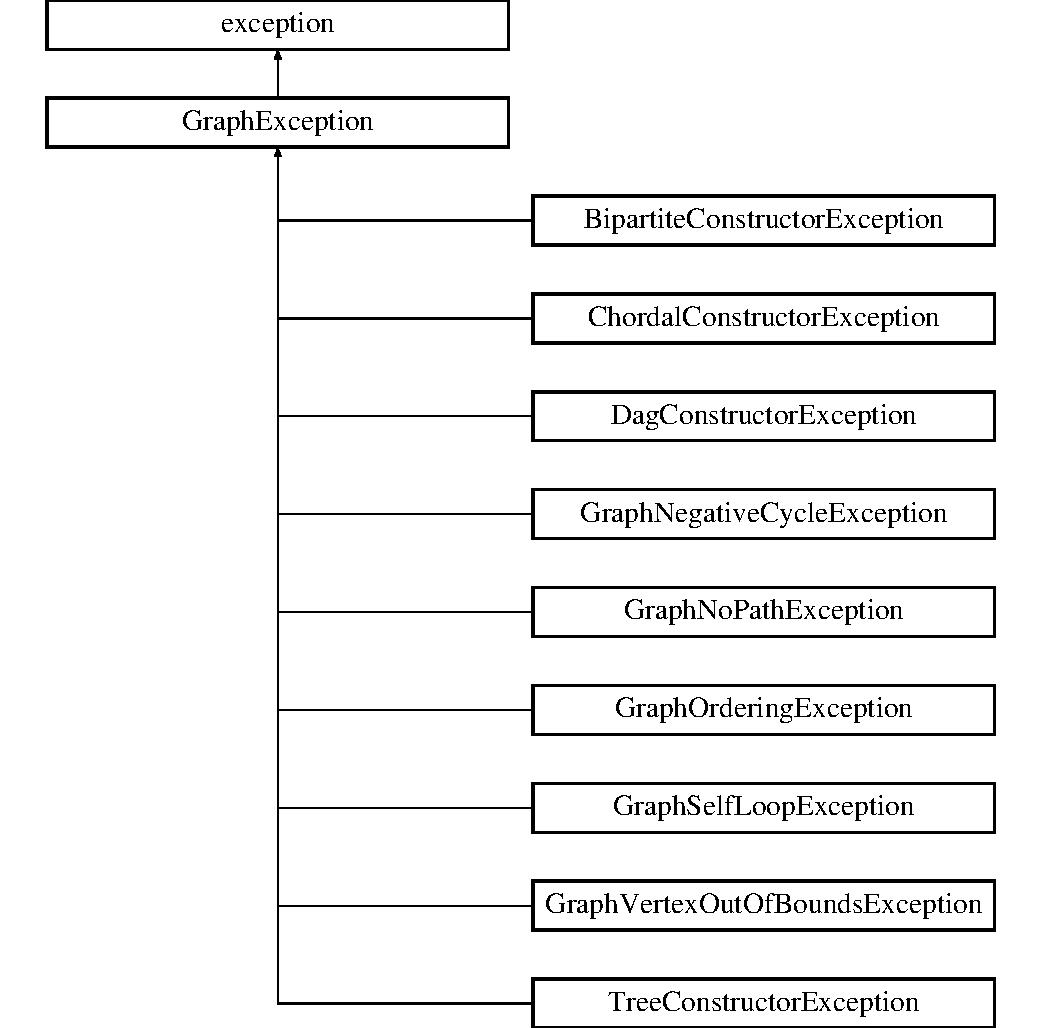
\includegraphics[height=11.000000cm]{classGraphException}
\end{center}
\end{figure}
\doxysubsection*{Membros públicos}
\begin{DoxyCompactItemize}
\item 
\mbox{\Hypertarget{classGraphException_ad4368b8af89252086b225cedcfc38639}\label{classGraphException_ad4368b8af89252086b225cedcfc38639}} 
const char $\ast$ \mbox{\hyperlink{classGraphException_ad4368b8af89252086b225cedcfc38639}{what}} () const  throw ()
\begin{DoxyCompactList}\small\item\em Retorna a mensagem de erro da exceção. \end{DoxyCompactList}\end{DoxyCompactItemize}


\doxysubsection{Descrição detalhada}
Classe de exceções de grafos. 

A documentação para esta classe foi gerada a partir do seguinte ficheiro\+:\begin{DoxyCompactItemize}
\item 
include/models/graph/\mbox{\hyperlink{GraphGen_8hpp}{Graph\+Gen.\+hpp}}\end{DoxyCompactItemize}

\hypertarget{classGraphGen}{}\section{Referência à classe Graph\+Gen}
\label{classGraphGen}\index{Graph\+Gen@{Graph\+Gen}}


Classe para grafos gerais.  




{\ttfamily \#include $<$Graph\+Gen.\+hpp$>$}

Diagrama de heranças da classe Graph\+Gen\begin{figure}[H]
\begin{center}
\leavevmode
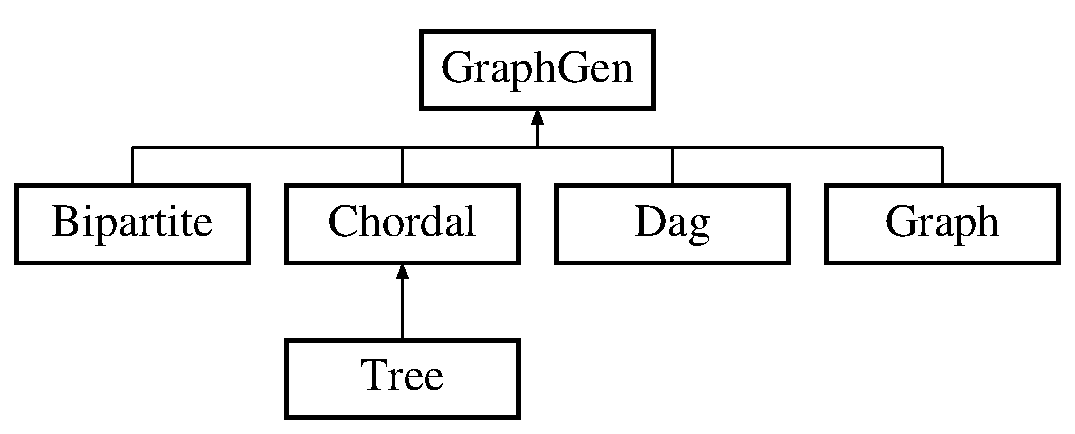
\includegraphics[height=3.000000cm]{classGraphGen}
\end{center}
\end{figure}
\subsection*{Membros públicos}
\begin{DoxyCompactItemize}
\item 
\mbox{\Hypertarget{classGraphGen_a71eb825043c2518df1be9a0ccef36bcb}\label{classGraphGen_a71eb825043c2518df1be9a0ccef36bcb}} 
\hyperlink{classGraphGen_a71eb825043c2518df1be9a0ccef36bcb}{Graph\+Gen} ()
\begin{DoxyCompactList}\small\item\em Construtor para o grafo vazio. \end{DoxyCompactList}\item 
\hyperlink{classGraphGen_aec08708894158ba3098873e7a1da6b60}{Graph\+Gen} (int)
\item 
\hyperlink{classGraphGen_abdb70c362c414ff5a18ab3796126a1a9}{Graph\+Gen} (int, vector$<$ string $>$ \&)
\item 
int \hyperlink{classGraphGen_a7447dc2fdc4cd3f86579811febfff1ad}{getN} ()
\item 
int \hyperlink{classGraphGen_aad12bcf774a0fa97150b01126d3a3e90}{getM} ()
\item 
vector$<$ vector$<$ pair$<$ int, int $>$ $>$ $>$ \hyperlink{classGraphGen_a36741424a266249c915f29fbab96175c}{get\+Adj} ()
\item 
vector$<$ vector$<$ pair$<$ int, int $>$ $>$ $>$ \hyperlink{classGraphGen_ab37943d4526c45711622796c84e983ac}{get\+Sim\+Adj} ()
\item 
vector$<$ pair$<$ int, int $>$ $>$ \hyperlink{classGraphGen_af140b74e5bbb7171a0b76f73d10c14ae}{get\+Edges} ()
\item 
vector$<$ int $>$ \hyperlink{classGraphGen_a56cb589bfd48135fe224d172dbed3155}{get\+Pesos} ()
\item 
vector$<$ vector$<$ int $>$ $>$ \hyperlink{classGraphGen_a32029b7e5e2c379bdc5412f0e954e121}{get\+Matrix} ()
\item 
vector$<$ vector$<$ int $>$ $>$ \hyperlink{classGraphGen_ab2f8872fc9fab4268ad999dd89e1d4fa}{get\+Sim\+Matrix} ()
\item 
bool \hyperlink{classGraphGen_aa0069b56cfa3e2d7d596bda9ba4ccc2b}{is\+Weighted} ()
\item 
bool \hyperlink{classGraphGen_a904cd0ab02e4c837ebd85226996fb4b2}{has\+Negative\+Weight} ()
\item 
bool \hyperlink{classGraphGen_a4fba74f3a12a3153843f550569981b0b}{reaches} (int, int)
\item 
bool \hyperlink{classGraphGen_addc27f1b1daa452bb0943c867b550906}{is\+Connected} ()
\item 
bool \hyperlink{classGraphGen_a41afdf97face9260e82749c4c770b2e7}{is\+Bipartite} ()
\item 
bool \hyperlink{classGraphGen_aac3e93061f340c6855aa54ed73922f47}{is\+Chordal} ()
\item 
bool \hyperlink{classGraphGen_ab4923b690b5fe013f35377b849bb6609}{is\+Dag} ()
\item 
bool \hyperlink{classGraphGen_adffd99540a68b2c158cc1b089ccfd550}{is\+Tree} ()
\item 
vector$<$ int $>$ \hyperlink{classGraphGen_a875733956a1f667d68afb420f53ecc86}{scc} ()
\item 
long long \hyperlink{classGraphGen_ad42fcde82e163baadcfaa02293242db5}{shortest\+Path} (int, int)
\item 
virtual vector$<$ int $>$ \hyperlink{classGraphGen_ad44c80646f694460fafa3e3657beb4d0}{coloring} ()
\item 
vector$<$ int $>$ \hyperlink{classGraphGen_a8505ba4cbaa0685f43e52a4c4f296dc1}{greedy\+Coloring} ()
\item 
vector$<$ int $>$ \hyperlink{classGraphGen_a0690c98ce5c9dd544074f690fb79a8c6}{greedy\+Coloring} (vector$<$ int $>$)
\item 
vector$<$ bool $>$ \hyperlink{classGraphGen_abfc9e2946585f5ea7e2948cd724d37e8}{art\+Points} ()
\item 
vector$<$ pair$<$ int, int $>$ $>$ \hyperlink{classGraphGen_ac80b65f7234db5bc163c7736aa0f561a}{bridges} ()
\end{DoxyCompactItemize}
\subsection*{Atributos Públicos}
\begin{DoxyCompactItemize}
\item 
\mbox{\Hypertarget{classGraphGen_a59a950a3a5b8d5f3bda7b544a83248ed}\label{classGraphGen_a59a950a3a5b8d5f3bda7b544a83248ed}} 
vector$<$ string $>$ \hyperlink{classGraphGen_a59a950a3a5b8d5f3bda7b544a83248ed}{label}
\begin{DoxyCompactList}\small\item\em Lista de rótulos dos vértices. \end{DoxyCompactList}\end{DoxyCompactItemize}
\subsection*{Membros protegidos}
\begin{DoxyCompactItemize}
\item 
pair$<$ vector$<$ int $>$, vector$<$ int $>$ $>$ \hyperlink{classGraphGen_a7811947062c0aa0fd1c56af0442dc9ad}{maximum\+Cardinality\+Search} ()
\item 
bool \hyperlink{classGraphGen_ad22d4dd7a1006663e1ba653c16b26e1a}{zero\+Fill\+In} (pair$<$ vector$<$ int $>$, vector$<$ int $>$$>$)
\item 
\mbox{\Hypertarget{classGraphGen_ac4ae31e7a52c9b2227ab8deb47d091a5}\label{classGraphGen_ac4ae31e7a52c9b2227ab8deb47d091a5}} 
bool \hyperlink{classGraphGen_ac4ae31e7a52c9b2227ab8deb47d091a5}{check\+Ordering} (vector$<$ int $>$)
\begin{DoxyCompactList}\small\item\em Verifica se uma ordenação atende às exigências de uma ordenação. \end{DoxyCompactList}\end{DoxyCompactItemize}
\subsection*{Atributos Protegidos}
\begin{DoxyCompactItemize}
\item 
\mbox{\Hypertarget{classGraphGen_af0087a36d5f72076ae87b0f9022c0033}\label{classGraphGen_af0087a36d5f72076ae87b0f9022c0033}} 
int \hyperlink{classGraphGen_af0087a36d5f72076ae87b0f9022c0033}{n}
\begin{DoxyCompactList}\small\item\em Número de vértices do grafo. \end{DoxyCompactList}\item 
\mbox{\Hypertarget{classGraphGen_aa313851fc05ee0f7a2ce768ba296e944}\label{classGraphGen_aa313851fc05ee0f7a2ce768ba296e944}} 
int \hyperlink{classGraphGen_aa313851fc05ee0f7a2ce768ba296e944}{m}
\begin{DoxyCompactList}\small\item\em Número de arestas do grafo. \end{DoxyCompactList}\item 
\mbox{\Hypertarget{classGraphGen_ae1cc2cf59230c1cdff45fa6848f1bf1f}\label{classGraphGen_ae1cc2cf59230c1cdff45fa6848f1bf1f}} 
vector$<$ vector$<$ pair$<$ int, int $>$ $>$ $>$ \hyperlink{classGraphGen_ae1cc2cf59230c1cdff45fa6848f1bf1f}{adj}
\begin{DoxyCompactList}\small\item\em Lista de adjacência direcionada. \end{DoxyCompactList}\item 
\mbox{\Hypertarget{classGraphGen_a6bfecbfc2aca704e5107dd667a23a1c0}\label{classGraphGen_a6bfecbfc2aca704e5107dd667a23a1c0}} 
vector$<$ vector$<$ pair$<$ int, int $>$ $>$ $>$ \hyperlink{classGraphGen_a6bfecbfc2aca704e5107dd667a23a1c0}{sim\+Adj}
\begin{DoxyCompactList}\small\item\em Lista de adjacência não direcionada. \end{DoxyCompactList}\end{DoxyCompactItemize}


\subsection{Descrição detalhada}
Classe para grafos gerais. 

\subsection{Documentação dos Construtores \& Destrutor}
\mbox{\Hypertarget{classGraphGen_aec08708894158ba3098873e7a1da6b60}\label{classGraphGen_aec08708894158ba3098873e7a1da6b60}} 
\index{Graph\+Gen@{Graph\+Gen}!Graph\+Gen@{Graph\+Gen}}
\index{Graph\+Gen@{Graph\+Gen}!Graph\+Gen@{Graph\+Gen}}
\subsubsection{\texorpdfstring{Graph\+Gen()}{GraphGen()}\hspace{0.1cm}{\footnotesize\ttfamily [1/2]}}
{\footnotesize\ttfamily Graph\+Gen\+::\+Graph\+Gen (\begin{DoxyParamCaption}\item[{int}]{ }\end{DoxyParamCaption})}

Construtor para o grafo por número de vértices. 
\begin{DoxyParams}{Parâmetros}
{\em Número} & de vértices. \\
\hline
\end{DoxyParams}
\mbox{\Hypertarget{classGraphGen_abdb70c362c414ff5a18ab3796126a1a9}\label{classGraphGen_abdb70c362c414ff5a18ab3796126a1a9}} 
\index{Graph\+Gen@{Graph\+Gen}!Graph\+Gen@{Graph\+Gen}}
\index{Graph\+Gen@{Graph\+Gen}!Graph\+Gen@{Graph\+Gen}}
\subsubsection{\texorpdfstring{Graph\+Gen()}{GraphGen()}\hspace{0.1cm}{\footnotesize\ttfamily [2/2]}}
{\footnotesize\ttfamily Graph\+Gen\+::\+Graph\+Gen (\begin{DoxyParamCaption}\item[{int}]{,  }\item[{vector$<$ string $>$ \&}]{ }\end{DoxyParamCaption})}

Construtor para o grafo por número de vértices e seus rótulos. 
\begin{DoxyParams}{Parâmetros}
{\em Número} & de vértices. \\
\hline
{\em Lista} & de rótulos. \\
\hline
\end{DoxyParams}


\subsection{Documentação dos métodos}
\mbox{\Hypertarget{classGraphGen_abfc9e2946585f5ea7e2948cd724d37e8}\label{classGraphGen_abfc9e2946585f5ea7e2948cd724d37e8}} 
\index{Graph\+Gen@{Graph\+Gen}!art\+Points@{art\+Points}}
\index{art\+Points@{art\+Points}!Graph\+Gen@{Graph\+Gen}}
\subsubsection{\texorpdfstring{art\+Points()}{artPoints()}}
{\footnotesize\ttfamily vector$<$bool$>$ Graph\+Gen\+::art\+Points (\begin{DoxyParamCaption}{ }\end{DoxyParamCaption})}

Retorna um vetor de booleanos que informa se cada vértice é um ponto de articulação

Complexidade\+: O(n + m) \begin{DoxyReturn}{Retorna}
Lista informando se cada vértice é ponto de articulação ou não. 
\end{DoxyReturn}
\mbox{\Hypertarget{classGraphGen_ac80b65f7234db5bc163c7736aa0f561a}\label{classGraphGen_ac80b65f7234db5bc163c7736aa0f561a}} 
\index{Graph\+Gen@{Graph\+Gen}!bridges@{bridges}}
\index{bridges@{bridges}!Graph\+Gen@{Graph\+Gen}}
\subsubsection{\texorpdfstring{bridges()}{bridges()}}
{\footnotesize\ttfamily vector$<$pair$<$int, int$>$ $>$ Graph\+Gen\+::bridges (\begin{DoxyParamCaption}{ }\end{DoxyParamCaption})}

Retorna um vetor de booleanos que informa se cada aresta é uma ponte

Complexidade\+: O(n + m) \begin{DoxyReturn}{Retorna}
Lista com as arestas que são pontes no grafo. 
\end{DoxyReturn}
\mbox{\Hypertarget{classGraphGen_ad44c80646f694460fafa3e3657beb4d0}\label{classGraphGen_ad44c80646f694460fafa3e3657beb4d0}} 
\index{Graph\+Gen@{Graph\+Gen}!coloring@{coloring}}
\index{coloring@{coloring}!Graph\+Gen@{Graph\+Gen}}
\subsubsection{\texorpdfstring{coloring()}{coloring()}}
{\footnotesize\ttfamily virtual vector$<$int$>$ Graph\+Gen\+::coloring (\begin{DoxyParamCaption}{ }\end{DoxyParamCaption})\hspace{0.3cm}{\ttfamily [virtual]}}

Retorna uma lista com a cor de cada vértice em uma coloração mínima.

Complexidade\+: O(nlog(n) + m) quando cordal \begin{DoxyReturn}{Retorna}
Lista com a cor de cada vértice. 
\end{DoxyReturn}


Reimplementado em \hyperlink{classChordal_acac4822a1eb3376c29f3d193baaec91f}{Chordal}.

\mbox{\Hypertarget{classGraphGen_a36741424a266249c915f29fbab96175c}\label{classGraphGen_a36741424a266249c915f29fbab96175c}} 
\index{Graph\+Gen@{Graph\+Gen}!get\+Adj@{get\+Adj}}
\index{get\+Adj@{get\+Adj}!Graph\+Gen@{Graph\+Gen}}
\subsubsection{\texorpdfstring{get\+Adj()}{getAdj()}}
{\footnotesize\ttfamily vector$<$vector$<$pair$<$int, int$>$ $>$ $>$ Graph\+Gen\+::get\+Adj (\begin{DoxyParamCaption}{ }\end{DoxyParamCaption})}

Retorna a lista de adjacência direcionada. \begin{DoxyReturn}{Retorna}
Lista de adjacência direcionada do grafo. 
\end{DoxyReturn}
\mbox{\Hypertarget{classGraphGen_af140b74e5bbb7171a0b76f73d10c14ae}\label{classGraphGen_af140b74e5bbb7171a0b76f73d10c14ae}} 
\index{Graph\+Gen@{Graph\+Gen}!get\+Edges@{get\+Edges}}
\index{get\+Edges@{get\+Edges}!Graph\+Gen@{Graph\+Gen}}
\subsubsection{\texorpdfstring{get\+Edges()}{getEdges()}}
{\footnotesize\ttfamily vector$<$pair$<$int, int$>$ $>$ Graph\+Gen\+::get\+Edges (\begin{DoxyParamCaption}{ }\end{DoxyParamCaption})}

Retorna a lista das arestas. \begin{DoxyReturn}{Retorna}
Lista com as arestas do grafo. 
\end{DoxyReturn}
\mbox{\Hypertarget{classGraphGen_aad12bcf774a0fa97150b01126d3a3e90}\label{classGraphGen_aad12bcf774a0fa97150b01126d3a3e90}} 
\index{Graph\+Gen@{Graph\+Gen}!getM@{getM}}
\index{getM@{getM}!Graph\+Gen@{Graph\+Gen}}
\subsubsection{\texorpdfstring{get\+M()}{getM()}}
{\footnotesize\ttfamily int Graph\+Gen\+::getM (\begin{DoxyParamCaption}{ }\end{DoxyParamCaption})}

Retorn o número de arestas. \begin{DoxyReturn}{Retorna}
Número de arestas do grafo. 
\end{DoxyReturn}
\mbox{\Hypertarget{classGraphGen_a32029b7e5e2c379bdc5412f0e954e121}\label{classGraphGen_a32029b7e5e2c379bdc5412f0e954e121}} 
\index{Graph\+Gen@{Graph\+Gen}!get\+Matrix@{get\+Matrix}}
\index{get\+Matrix@{get\+Matrix}!Graph\+Gen@{Graph\+Gen}}
\subsubsection{\texorpdfstring{get\+Matrix()}{getMatrix()}}
{\footnotesize\ttfamily vector$<$vector$<$int$>$ $>$ Graph\+Gen\+::get\+Matrix (\begin{DoxyParamCaption}{ }\end{DoxyParamCaption})}

Retorna a matriz de adjacência. \begin{DoxyReturn}{Retorna}
Matriz de adjacência do grafo. 
\end{DoxyReturn}
\mbox{\Hypertarget{classGraphGen_a7447dc2fdc4cd3f86579811febfff1ad}\label{classGraphGen_a7447dc2fdc4cd3f86579811febfff1ad}} 
\index{Graph\+Gen@{Graph\+Gen}!getN@{getN}}
\index{getN@{getN}!Graph\+Gen@{Graph\+Gen}}
\subsubsection{\texorpdfstring{get\+N()}{getN()}}
{\footnotesize\ttfamily int Graph\+Gen\+::getN (\begin{DoxyParamCaption}{ }\end{DoxyParamCaption})}

Retorna o número de vértices \begin{DoxyReturn}{Retorna}
Número de vértices do grafo. 
\end{DoxyReturn}
\mbox{\Hypertarget{classGraphGen_a56cb589bfd48135fe224d172dbed3155}\label{classGraphGen_a56cb589bfd48135fe224d172dbed3155}} 
\index{Graph\+Gen@{Graph\+Gen}!get\+Pesos@{get\+Pesos}}
\index{get\+Pesos@{get\+Pesos}!Graph\+Gen@{Graph\+Gen}}
\subsubsection{\texorpdfstring{get\+Pesos()}{getPesos()}}
{\footnotesize\ttfamily vector$<$int$>$ Graph\+Gen\+::get\+Pesos (\begin{DoxyParamCaption}{ }\end{DoxyParamCaption})}

Retorna a lista de pesos das arestas. \begin{DoxyReturn}{Retorna}
lista com os pesos do grafo. 
\end{DoxyReturn}
\mbox{\Hypertarget{classGraphGen_ab37943d4526c45711622796c84e983ac}\label{classGraphGen_ab37943d4526c45711622796c84e983ac}} 
\index{Graph\+Gen@{Graph\+Gen}!get\+Sim\+Adj@{get\+Sim\+Adj}}
\index{get\+Sim\+Adj@{get\+Sim\+Adj}!Graph\+Gen@{Graph\+Gen}}
\subsubsection{\texorpdfstring{get\+Sim\+Adj()}{getSimAdj()}}
{\footnotesize\ttfamily vector$<$vector$<$pair$<$int, int$>$ $>$ $>$ Graph\+Gen\+::get\+Sim\+Adj (\begin{DoxyParamCaption}{ }\end{DoxyParamCaption})}

Retorn a lista de adjacência não direcionada. \begin{DoxyReturn}{Retorna}
Lista de adjacêncai não direcionada do grafo. 
\end{DoxyReturn}
\mbox{\Hypertarget{classGraphGen_ab2f8872fc9fab4268ad999dd89e1d4fa}\label{classGraphGen_ab2f8872fc9fab4268ad999dd89e1d4fa}} 
\index{Graph\+Gen@{Graph\+Gen}!get\+Sim\+Matrix@{get\+Sim\+Matrix}}
\index{get\+Sim\+Matrix@{get\+Sim\+Matrix}!Graph\+Gen@{Graph\+Gen}}
\subsubsection{\texorpdfstring{get\+Sim\+Matrix()}{getSimMatrix()}}
{\footnotesize\ttfamily vector$<$vector$<$int$>$ $>$ Graph\+Gen\+::get\+Sim\+Matrix (\begin{DoxyParamCaption}{ }\end{DoxyParamCaption})}

Retorna a matriz de adjacência simétrica. \begin{DoxyReturn}{Retorna}
Matriz de adjacência simétrica. 
\end{DoxyReturn}
\mbox{\Hypertarget{classGraphGen_a8505ba4cbaa0685f43e52a4c4f296dc1}\label{classGraphGen_a8505ba4cbaa0685f43e52a4c4f296dc1}} 
\index{Graph\+Gen@{Graph\+Gen}!greedy\+Coloring@{greedy\+Coloring}}
\index{greedy\+Coloring@{greedy\+Coloring}!Graph\+Gen@{Graph\+Gen}}
\subsubsection{\texorpdfstring{greedy\+Coloring()}{greedyColoring()}\hspace{0.1cm}{\footnotesize\ttfamily [1/2]}}
{\footnotesize\ttfamily vector$<$int$>$ Graph\+Gen\+::greedy\+Coloring (\begin{DoxyParamCaption}{ }\end{DoxyParamCaption})}

Retorna uma lista com a cor de cada vértice em uma coloração gulosa na ordem dos vértices.

Complexidade\+: O(n + m) \begin{DoxyReturn}{Retorna}
Lista com a cor de cada vértice. 
\end{DoxyReturn}
\mbox{\Hypertarget{classGraphGen_a0690c98ce5c9dd544074f690fb79a8c6}\label{classGraphGen_a0690c98ce5c9dd544074f690fb79a8c6}} 
\index{Graph\+Gen@{Graph\+Gen}!greedy\+Coloring@{greedy\+Coloring}}
\index{greedy\+Coloring@{greedy\+Coloring}!Graph\+Gen@{Graph\+Gen}}
\subsubsection{\texorpdfstring{greedy\+Coloring()}{greedyColoring()}\hspace{0.1cm}{\footnotesize\ttfamily [2/2]}}
{\footnotesize\ttfamily vector$<$int$>$ Graph\+Gen\+::greedy\+Coloring (\begin{DoxyParamCaption}\item[{vector$<$ int $>$}]{ }\end{DoxyParamCaption})}

Retorna uma lista com a cor de cada vértice em uma coloração gulosa para uma dada ordem dos vértices.

Complexidade\+: O(n + m) 
\begin{DoxyParams}{Parâmetros}
{\em Ordem} & para avaliação do algoritmo guloso. \\
\hline
\end{DoxyParams}
\begin{DoxyReturn}{Retorna}
Lista com a cor de cada vértice. 
\end{DoxyReturn}
\mbox{\Hypertarget{classGraphGen_a904cd0ab02e4c837ebd85226996fb4b2}\label{classGraphGen_a904cd0ab02e4c837ebd85226996fb4b2}} 
\index{Graph\+Gen@{Graph\+Gen}!has\+Negative\+Weight@{has\+Negative\+Weight}}
\index{has\+Negative\+Weight@{has\+Negative\+Weight}!Graph\+Gen@{Graph\+Gen}}
\subsubsection{\texorpdfstring{has\+Negative\+Weight()}{hasNegativeWeight()}}
{\footnotesize\ttfamily bool Graph\+Gen\+::has\+Negative\+Weight (\begin{DoxyParamCaption}{ }\end{DoxyParamCaption})}

Retorna se o grafo possui arestas com pesos negativos. \begin{DoxyReturn}{Retorna}
bool informando se o grafo possui peso negativo. 
\end{DoxyReturn}
\mbox{\Hypertarget{classGraphGen_a41afdf97face9260e82749c4c770b2e7}\label{classGraphGen_a41afdf97face9260e82749c4c770b2e7}} 
\index{Graph\+Gen@{Graph\+Gen}!is\+Bipartite@{is\+Bipartite}}
\index{is\+Bipartite@{is\+Bipartite}!Graph\+Gen@{Graph\+Gen}}
\subsubsection{\texorpdfstring{is\+Bipartite()}{isBipartite()}}
{\footnotesize\ttfamily bool Graph\+Gen\+::is\+Bipartite (\begin{DoxyParamCaption}{ }\end{DoxyParamCaption})}

Retorna se o grafo é bipartido. \begin{DoxyReturn}{Retorna}
bool informando se o grafo é bipartido. 
\end{DoxyReturn}
\mbox{\Hypertarget{classGraphGen_aac3e93061f340c6855aa54ed73922f47}\label{classGraphGen_aac3e93061f340c6855aa54ed73922f47}} 
\index{Graph\+Gen@{Graph\+Gen}!is\+Chordal@{is\+Chordal}}
\index{is\+Chordal@{is\+Chordal}!Graph\+Gen@{Graph\+Gen}}
\subsubsection{\texorpdfstring{is\+Chordal()}{isChordal()}}
{\footnotesize\ttfamily bool Graph\+Gen\+::is\+Chordal (\begin{DoxyParamCaption}{ }\end{DoxyParamCaption})}

Retorna se o grafo é cordal. \begin{DoxyReturn}{Retorna}
bool informando se o grafo é cordal. 
\end{DoxyReturn}
\mbox{\Hypertarget{classGraphGen_addc27f1b1daa452bb0943c867b550906}\label{classGraphGen_addc27f1b1daa452bb0943c867b550906}} 
\index{Graph\+Gen@{Graph\+Gen}!is\+Connected@{is\+Connected}}
\index{is\+Connected@{is\+Connected}!Graph\+Gen@{Graph\+Gen}}
\subsubsection{\texorpdfstring{is\+Connected()}{isConnected()}}
{\footnotesize\ttfamily bool Graph\+Gen\+::is\+Connected (\begin{DoxyParamCaption}{ }\end{DoxyParamCaption})}

Retorna se o grafo é conexo. \begin{DoxyReturn}{Retorna}
bool informando se o grafo é conexo. 
\end{DoxyReturn}
\mbox{\Hypertarget{classGraphGen_ab4923b690b5fe013f35377b849bb6609}\label{classGraphGen_ab4923b690b5fe013f35377b849bb6609}} 
\index{Graph\+Gen@{Graph\+Gen}!is\+Dag@{is\+Dag}}
\index{is\+Dag@{is\+Dag}!Graph\+Gen@{Graph\+Gen}}
\subsubsection{\texorpdfstring{is\+Dag()}{isDag()}}
{\footnotesize\ttfamily bool Graph\+Gen\+::is\+Dag (\begin{DoxyParamCaption}{ }\end{DoxyParamCaption})}

Retorna se o grafo é direcionado acíclico. \begin{DoxyReturn}{Retorna}
bool informando se o grafo é D\+AG. 
\end{DoxyReturn}
\mbox{\Hypertarget{classGraphGen_adffd99540a68b2c158cc1b089ccfd550}\label{classGraphGen_adffd99540a68b2c158cc1b089ccfd550}} 
\index{Graph\+Gen@{Graph\+Gen}!is\+Tree@{is\+Tree}}
\index{is\+Tree@{is\+Tree}!Graph\+Gen@{Graph\+Gen}}
\subsubsection{\texorpdfstring{is\+Tree()}{isTree()}}
{\footnotesize\ttfamily bool Graph\+Gen\+::is\+Tree (\begin{DoxyParamCaption}{ }\end{DoxyParamCaption})}

Retorna se o grafo é uma árvore. \begin{DoxyReturn}{Retorna}
bool informando se o grafo é uma árvore. 
\end{DoxyReturn}
\mbox{\Hypertarget{classGraphGen_aa0069b56cfa3e2d7d596bda9ba4ccc2b}\label{classGraphGen_aa0069b56cfa3e2d7d596bda9ba4ccc2b}} 
\index{Graph\+Gen@{Graph\+Gen}!is\+Weighted@{is\+Weighted}}
\index{is\+Weighted@{is\+Weighted}!Graph\+Gen@{Graph\+Gen}}
\subsubsection{\texorpdfstring{is\+Weighted()}{isWeighted()}}
{\footnotesize\ttfamily bool Graph\+Gen\+::is\+Weighted (\begin{DoxyParamCaption}{ }\end{DoxyParamCaption})}

Retorna se o grafo possui arestas com pesos. \begin{DoxyReturn}{Retorna}
bool informando se o grafo possui peso nas arestas. 
\end{DoxyReturn}
\mbox{\Hypertarget{classGraphGen_a7811947062c0aa0fd1c56af0442dc9ad}\label{classGraphGen_a7811947062c0aa0fd1c56af0442dc9ad}} 
\index{Graph\+Gen@{Graph\+Gen}!maximum\+Cardinality\+Search@{maximum\+Cardinality\+Search}}
\index{maximum\+Cardinality\+Search@{maximum\+Cardinality\+Search}!Graph\+Gen@{Graph\+Gen}}
\subsubsection{\texorpdfstring{maximum\+Cardinality\+Search()}{maximumCardinalitySearch()}}
{\footnotesize\ttfamily pair$<$vector$<$int$>$, vector$<$int$>$ $>$ Graph\+Gen\+::maximum\+Cardinality\+Search (\begin{DoxyParamCaption}{ }\end{DoxyParamCaption})\hspace{0.3cm}{\ttfamily [protected]}}

Retorna uma ordenação dos vértices, e sua ordenação inversa, de máxima caridinalidade (uma ordenação simplicial se e somente se o grafo for cordal).

Complexidade\+: O(nlog(n) + m) \mbox{\Hypertarget{classGraphGen_a4fba74f3a12a3153843f550569981b0b}\label{classGraphGen_a4fba74f3a12a3153843f550569981b0b}} 
\index{Graph\+Gen@{Graph\+Gen}!reaches@{reaches}}
\index{reaches@{reaches}!Graph\+Gen@{Graph\+Gen}}
\subsubsection{\texorpdfstring{reaches()}{reaches()}}
{\footnotesize\ttfamily bool Graph\+Gen\+::reaches (\begin{DoxyParamCaption}\item[{int}]{,  }\item[{int}]{ }\end{DoxyParamCaption})}

Retorna se dois vértices se alcançam. 
\begin{DoxyParams}{Parâmetros}
{\em Vértice} & a. \\
\hline
{\em Vértice} & b. \\
\hline
\end{DoxyParams}
\begin{DoxyReturn}{Retorna}
bool informando se o vértice \textquotesingle{}a\textquotesingle{} alcança o vértice \textquotesingle{}b\textquotesingle{}. 
\end{DoxyReturn}
\mbox{\Hypertarget{classGraphGen_a875733956a1f667d68afb420f53ecc86}\label{classGraphGen_a875733956a1f667d68afb420f53ecc86}} 
\index{Graph\+Gen@{Graph\+Gen}!scc@{scc}}
\index{scc@{scc}!Graph\+Gen@{Graph\+Gen}}
\subsubsection{\texorpdfstring{scc()}{scc()}}
{\footnotesize\ttfamily vector$<$int$>$ Graph\+Gen\+::scc (\begin{DoxyParamCaption}{ }\end{DoxyParamCaption})}

Retorna uma lista com a componente fortemente conexa de cada vértice.

Complexidade\+: O(n + m) \begin{DoxyReturn}{Retorna}
Lista tal que na posição \textquotesingle{}i\textquotesingle{}, possui o índice da componente fortemente conexa do vértice \textquotesingle{}i\textquotesingle{}. 
\end{DoxyReturn}
\mbox{\Hypertarget{classGraphGen_ad42fcde82e163baadcfaa02293242db5}\label{classGraphGen_ad42fcde82e163baadcfaa02293242db5}} 
\index{Graph\+Gen@{Graph\+Gen}!shortest\+Path@{shortest\+Path}}
\index{shortest\+Path@{shortest\+Path}!Graph\+Gen@{Graph\+Gen}}
\subsubsection{\texorpdfstring{shortest\+Path()}{shortestPath()}}
{\footnotesize\ttfamily long long Graph\+Gen\+::shortest\+Path (\begin{DoxyParamCaption}\item[{int}]{,  }\item[{int}]{ }\end{DoxyParamCaption})}

Retorna o menor caminho entre dois vértices.

Complexidade\+: se todos os pesos forem 1, linear. Se não houver peso negativo, O(m log(n)). Caso contrário, O(n$\ast$m). 
\begin{DoxyParams}{Parâmetros}
{\em Vértice} & \textquotesingle{}a\textquotesingle{}. \\
\hline
{\em Vértice} & \textquotesingle{}b\textquotesingle{}. \\
\hline
\end{DoxyParams}
\begin{DoxyReturn}{Retorna}
Comprimento do camínho mínimo de \textquotesingle{}a\textquotesingle{} até \textquotesingle{}b\textquotesingle{}. 
\end{DoxyReturn}
\mbox{\Hypertarget{classGraphGen_ad22d4dd7a1006663e1ba653c16b26e1a}\label{classGraphGen_ad22d4dd7a1006663e1ba653c16b26e1a}} 
\index{Graph\+Gen@{Graph\+Gen}!zero\+Fill\+In@{zero\+Fill\+In}}
\index{zero\+Fill\+In@{zero\+Fill\+In}!Graph\+Gen@{Graph\+Gen}}
\subsubsection{\texorpdfstring{zero\+Fill\+In()}{zeroFillIn()}}
{\footnotesize\ttfamily bool Graph\+Gen\+::zero\+Fill\+In (\begin{DoxyParamCaption}\item[{pair$<$ vector$<$ int $>$, vector$<$ int $>$$>$}]{ }\end{DoxyParamCaption})\hspace{0.3cm}{\ttfamily [protected]}}

Verifica se uma ordenação dos vértices (e sua ordenação inversa) possui as propriedades de de Zero-\/\+Fill-\/\+In (i.\+e., se o grafo é cordal).

Complexidade\+: O(n + m) 

A documentação para esta classe foi gerada a partir do seguinte ficheiro\+:\begin{DoxyCompactItemize}
\item 
include/models/graph/\hyperlink{GraphGen_8hpp}{Graph\+Gen.\+hpp}\end{DoxyCompactItemize}

\hypertarget{classGraphNegativeCycleException}{}\section{Referência à classe Graph\+Negative\+Cycle\+Exception}
\label{classGraphNegativeCycleException}\index{Graph\+Negative\+Cycle\+Exception@{Graph\+Negative\+Cycle\+Exception}}


Classe de exceções para ciclos negativos em caminhos mínimos.  




{\ttfamily \#include $<$Graph\+Gen.\+hpp$>$}

Diagrama de heranças da classe Graph\+Negative\+Cycle\+Exception\begin{figure}[H]
\begin{center}
\leavevmode
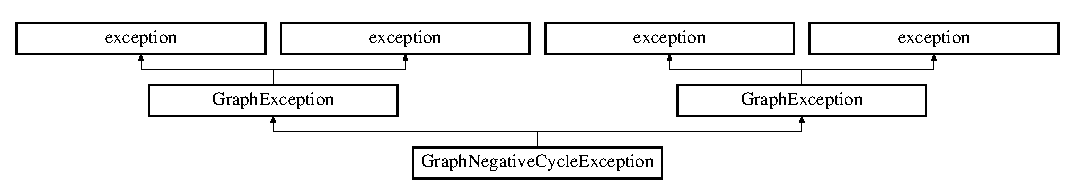
\includegraphics[height=3.000000cm]{classGraphNegativeCycleException}
\end{center}
\end{figure}
\subsection*{Membros públicos}
\begin{DoxyCompactItemize}
\item 
\mbox{\Hypertarget{classGraphNegativeCycleException_ae4862d8b8e61233ff35331fbe188f98d}\label{classGraphNegativeCycleException_ae4862d8b8e61233ff35331fbe188f98d}} 
\hyperlink{classGraphNegativeCycleException_ae4862d8b8e61233ff35331fbe188f98d}{Graph\+Negative\+Cycle\+Exception} ()
\begin{DoxyCompactList}\small\item\em Construtor para exceção de ciclos negativos. \end{DoxyCompactList}\item 
const char $\ast$ \hyperlink{classGraphNegativeCycleException_ae973328a57ec48ac66298365bfe7ded4}{what} () const  throw ()
\end{DoxyCompactItemize}


\subsection{Descrição detalhada}
Classe de exceções para ciclos negativos em caminhos mínimos. 

\subsection{Documentação dos métodos}
\mbox{\Hypertarget{classGraphNegativeCycleException_ae973328a57ec48ac66298365bfe7ded4}\label{classGraphNegativeCycleException_ae973328a57ec48ac66298365bfe7ded4}} 
\index{Graph\+Negative\+Cycle\+Exception@{Graph\+Negative\+Cycle\+Exception}!what@{what}}
\index{what@{what}!Graph\+Negative\+Cycle\+Exception@{Graph\+Negative\+Cycle\+Exception}}
\subsubsection{\texorpdfstring{what()}{what()}}
{\footnotesize\ttfamily const char$\ast$ Graph\+Negative\+Cycle\+Exception\+::what (\begin{DoxyParamCaption}{ }\end{DoxyParamCaption}) const throw  ) \hspace{0.3cm}{\ttfamily [inline]}}

Retorna a mensagem de erro da exceção. \begin{DoxyReturn}{Retorna}
Mensagem de erro. 
\end{DoxyReturn}


A documentação para esta classe foi gerada a partir do seguinte ficheiro\+:\begin{DoxyCompactItemize}
\item 
include/models/graph/\hyperlink{GraphGen_8hpp}{Graph\+Gen.\+hpp}\end{DoxyCompactItemize}

\hypertarget{classGraphNoPathException}{}\doxysection{Referência à classe Graph\+No\+Path\+Exception}
\label{classGraphNoPathException}\index{GraphNoPathException@{GraphNoPathException}}


Classe de exceções de ausência de caminho entre dois vértices.  




{\ttfamily \#include $<$Graph\+Gen.\+hpp$>$}

Diagrama de heranças da classe Graph\+No\+Path\+Exception\begin{figure}[H]
\begin{center}
\leavevmode
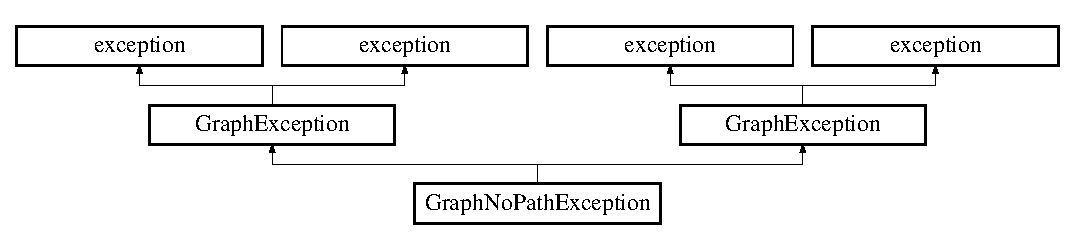
\includegraphics[height=3.000000cm]{classGraphNoPathException}
\end{center}
\end{figure}
\doxysubsection*{Membros públicos}
\begin{DoxyCompactItemize}
\item 
\mbox{\hyperlink{classGraphNoPathException_a1d9dd40f194e7705b8009cd2a4ed7f79}{Graph\+No\+Path\+Exception}} (int a, int b)
\item 
\mbox{\Hypertarget{classGraphNoPathException_a33d7ba709a76ad03175a929e8313221c}\label{classGraphNoPathException_a33d7ba709a76ad03175a929e8313221c}} 
const char $\ast$ \mbox{\hyperlink{classGraphNoPathException_a33d7ba709a76ad03175a929e8313221c}{what}} () const  throw ()
\begin{DoxyCompactList}\small\item\em Retorna a mensagem de erro da exceção. \end{DoxyCompactList}\end{DoxyCompactItemize}


\doxysubsection{Descrição detalhada}
Classe de exceções de ausência de caminho entre dois vértices. 

\doxysubsection{Documentação dos Construtores \& Destrutor}
\mbox{\Hypertarget{classGraphNoPathException_a1d9dd40f194e7705b8009cd2a4ed7f79}\label{classGraphNoPathException_a1d9dd40f194e7705b8009cd2a4ed7f79}} 
\index{GraphNoPathException@{GraphNoPathException}!GraphNoPathException@{GraphNoPathException}}
\index{GraphNoPathException@{GraphNoPathException}!GraphNoPathException@{GraphNoPathException}}
\doxysubsubsection{\texorpdfstring{GraphNoPathException()}{GraphNoPathException()}}
{\footnotesize\ttfamily Graph\+No\+Path\+Exception\+::\+Graph\+No\+Path\+Exception (\begin{DoxyParamCaption}\item[{int}]{a,  }\item[{int}]{b }\end{DoxyParamCaption})\hspace{0.3cm}{\ttfamily [inline]}}

Construtor para a exceção de ausência de caminho entre dois vértices 

A documentação para esta classe foi gerada a partir do seguinte ficheiro\+:\begin{DoxyCompactItemize}
\item 
include/models/graph/\mbox{\hyperlink{GraphGen_8hpp}{Graph\+Gen.\+hpp}}\end{DoxyCompactItemize}

\hypertarget{classGraphOrderingException}{}\doxysection{Referência à classe Graph\+Ordering\+Exception}
\label{classGraphOrderingException}\index{GraphOrderingException@{GraphOrderingException}}


Classe de exceções para ordenações de vértices fora do domínio.  




{\ttfamily \#include $<$Graph\+Gen.\+hpp$>$}

Diagrama de heranças da classe Graph\+Ordering\+Exception\begin{figure}[H]
\begin{center}
\leavevmode
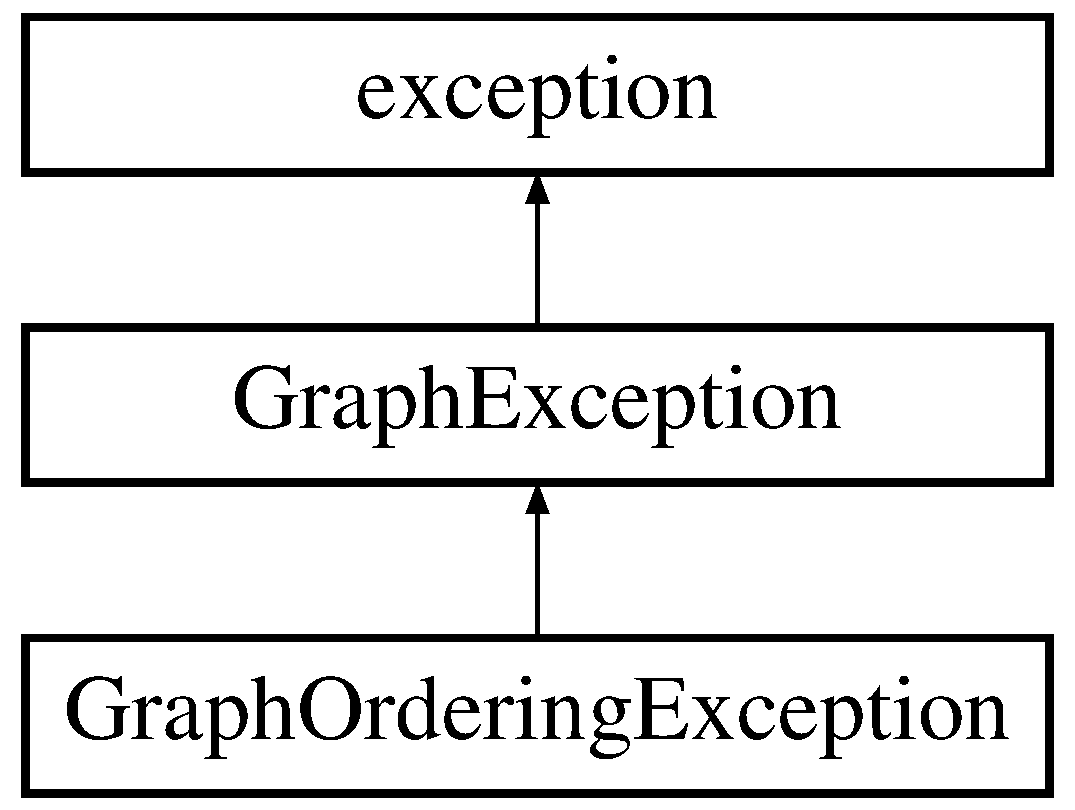
\includegraphics[height=3.000000cm]{classGraphOrderingException}
\end{center}
\end{figure}
\doxysubsection*{Membros públicos}
\begin{DoxyCompactItemize}
\item 
\mbox{\Hypertarget{classGraphOrderingException_a38d6f4e461cd40c0d2e8c07e7a5d6bef}\label{classGraphOrderingException_a38d6f4e461cd40c0d2e8c07e7a5d6bef}} 
const char $\ast$ \mbox{\hyperlink{classGraphOrderingException_a38d6f4e461cd40c0d2e8c07e7a5d6bef}{what}} () const  throw ()
\begin{DoxyCompactList}\small\item\em Retorna a mensagem de erro da exceção. \end{DoxyCompactList}\end{DoxyCompactItemize}


\doxysubsection{Descrição detalhada}
Classe de exceções para ordenações de vértices fora do domínio. 

A documentação para esta classe foi gerada a partir do seguinte ficheiro\+:\begin{DoxyCompactItemize}
\item 
include/models/graph/\mbox{\hyperlink{GraphGen_8hpp}{Graph\+Gen.\+hpp}}\end{DoxyCompactItemize}

\hypertarget{classGraphSelfLoopException}{}\section{Referência à classe Graph\+Self\+Loop\+Exception}
\label{classGraphSelfLoopException}\index{Graph\+Self\+Loop\+Exception@{Graph\+Self\+Loop\+Exception}}


Classe de exceções de laços.  




{\ttfamily \#include $<$Graph.\+hpp$>$}

Diagrama de heranças da classe Graph\+Self\+Loop\+Exception\begin{figure}[H]
\begin{center}
\leavevmode
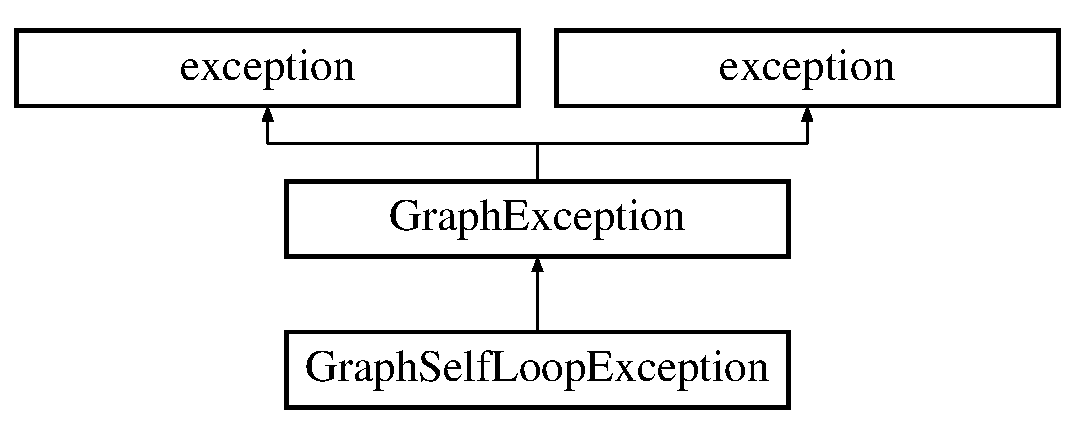
\includegraphics[height=3.000000cm]{classGraphSelfLoopException}
\end{center}
\end{figure}
\subsection*{Membros públicos}
\begin{DoxyCompactItemize}
\item 
\hyperlink{classGraphSelfLoopException_ad9e05922cf212c3fcd30426bf30f982e}{Graph\+Self\+Loop\+Exception} (int n)
\item 
const char $\ast$ \hyperlink{classGraphSelfLoopException_ae608d642082d2183111b8a43a1bfa64f}{what} () const  throw ()
\end{DoxyCompactItemize}


\subsection{Descrição detalhada}
Classe de exceções de laços. 

\subsection{Documentação dos Construtores \& Destrutor}
\mbox{\Hypertarget{classGraphSelfLoopException_ad9e05922cf212c3fcd30426bf30f982e}\label{classGraphSelfLoopException_ad9e05922cf212c3fcd30426bf30f982e}} 
\index{Graph\+Self\+Loop\+Exception@{Graph\+Self\+Loop\+Exception}!Graph\+Self\+Loop\+Exception@{Graph\+Self\+Loop\+Exception}}
\index{Graph\+Self\+Loop\+Exception@{Graph\+Self\+Loop\+Exception}!Graph\+Self\+Loop\+Exception@{Graph\+Self\+Loop\+Exception}}
\subsubsection{\texorpdfstring{Graph\+Self\+Loop\+Exception()}{GraphSelfLoopException()}}
{\footnotesize\ttfamily Graph\+Self\+Loop\+Exception\+::\+Graph\+Self\+Loop\+Exception (\begin{DoxyParamCaption}\item[{int}]{n }\end{DoxyParamCaption})\hspace{0.3cm}{\ttfamily [inline]}}

Construtor da exceção. 
\begin{DoxyParams}{Parâmetros}
{\em Vértice} & no qual o self-\/loop ocorreu. \\
\hline
\end{DoxyParams}


\subsection{Documentação dos métodos}
\mbox{\Hypertarget{classGraphSelfLoopException_ae608d642082d2183111b8a43a1bfa64f}\label{classGraphSelfLoopException_ae608d642082d2183111b8a43a1bfa64f}} 
\index{Graph\+Self\+Loop\+Exception@{Graph\+Self\+Loop\+Exception}!what@{what}}
\index{what@{what}!Graph\+Self\+Loop\+Exception@{Graph\+Self\+Loop\+Exception}}
\subsubsection{\texorpdfstring{what()}{what()}}
{\footnotesize\ttfamily const char$\ast$ Graph\+Self\+Loop\+Exception\+::what (\begin{DoxyParamCaption}{ }\end{DoxyParamCaption}) const throw  ) \hspace{0.3cm}{\ttfamily [inline]}}

Retorna a mensagem de erro da exceção. \begin{DoxyReturn}{Retorna}
Mensagem de erro. 
\end{DoxyReturn}


A documentação para esta classe foi gerada a partir do seguinte ficheiro\+:\begin{DoxyCompactItemize}
\item 
include/models/graph/\hyperlink{Graph_8hpp}{Graph.\+hpp}\end{DoxyCompactItemize}

\hypertarget{classGraphVertexOutOfBoundsException}{}\doxysection{Referência à classe Graph\+Vertex\+Out\+Of\+Bounds\+Exception}
\label{classGraphVertexOutOfBoundsException}\index{GraphVertexOutOfBoundsException@{GraphVertexOutOfBoundsException}}


Classe de exceções de vértice fora dos limites.  




{\ttfamily \#include $<$Graph.\+hpp$>$}

Diagrama de heranças da classe Graph\+Vertex\+Out\+Of\+Bounds\+Exception\begin{figure}[H]
\begin{center}
\leavevmode
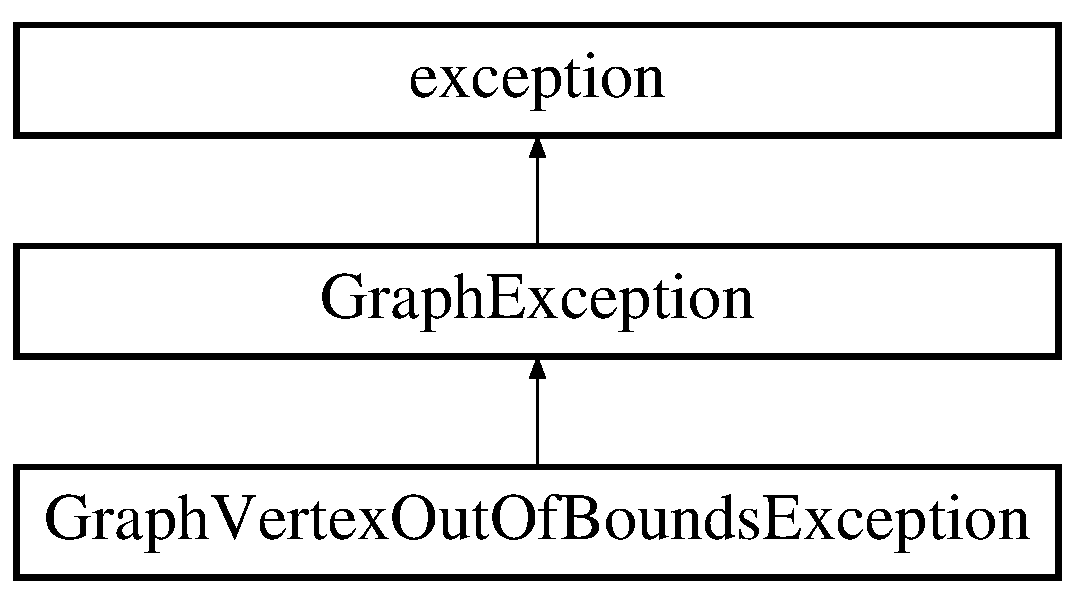
\includegraphics[height=3.000000cm]{classGraphVertexOutOfBoundsException}
\end{center}
\end{figure}
\doxysubsection*{Membros públicos}
\begin{DoxyCompactItemize}
\item 
\mbox{\Hypertarget{classGraphVertexOutOfBoundsException_a6f72cde302ff14c75138a7d1043d43e0}\label{classGraphVertexOutOfBoundsException_a6f72cde302ff14c75138a7d1043d43e0}} 
\mbox{\hyperlink{classGraphVertexOutOfBoundsException_a6f72cde302ff14c75138a7d1043d43e0}{Graph\+Vertex\+Out\+Of\+Bounds\+Exception}} (int n)
\begin{DoxyCompactList}\small\item\em Construtor da exceção. \end{DoxyCompactList}\item 
\mbox{\Hypertarget{classGraphVertexOutOfBoundsException_ac85fc95ea1c178023571adf7a9b8b0df}\label{classGraphVertexOutOfBoundsException_ac85fc95ea1c178023571adf7a9b8b0df}} 
const char $\ast$ \mbox{\hyperlink{classGraphVertexOutOfBoundsException_ac85fc95ea1c178023571adf7a9b8b0df}{what}} () const  throw ()
\begin{DoxyCompactList}\small\item\em Retorna a mensagem de erro da exceção. \end{DoxyCompactList}\end{DoxyCompactItemize}


\doxysubsection{Descrição detalhada}
Classe de exceções de vértice fora dos limites. 

A documentação para esta classe foi gerada a partir do seguinte ficheiro\+:\begin{DoxyCompactItemize}
\item 
include/models/graph/\mbox{\hyperlink{Graph_8hpp}{Graph.\+hpp}}\end{DoxyCompactItemize}

\hypertarget{classREPLException}{}\doxysection{Referência à classe R\+E\+P\+L\+Exception}
\label{classREPLException}\index{REPLException@{REPLException}}


Classe para exceções do R\+E\+PL.  




{\ttfamily \#include $<$Repl.\+hpp$>$}

Diagrama de heranças da classe R\+E\+P\+L\+Exception\begin{figure}[H]
\begin{center}
\leavevmode
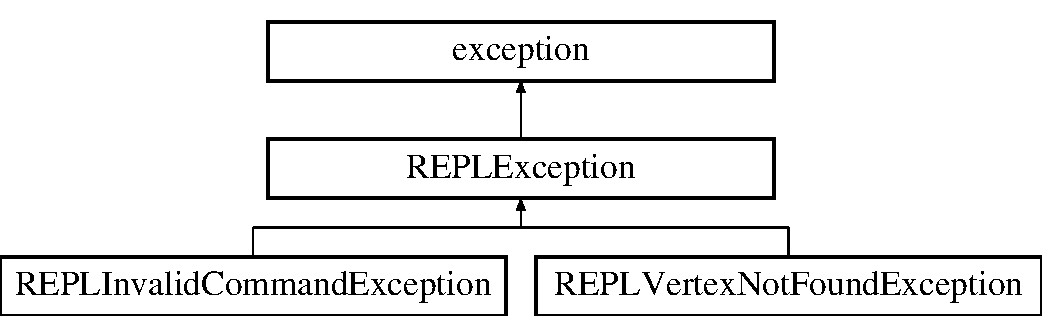
\includegraphics[height=3.000000cm]{classREPLException}
\end{center}
\end{figure}
\doxysubsection*{Membros públicos}
\begin{DoxyCompactItemize}
\item 
\mbox{\Hypertarget{classREPLException_abf6ea066b56e3730779929040b4f4762}\label{classREPLException_abf6ea066b56e3730779929040b4f4762}} 
\mbox{\hyperlink{classREPLException_abf6ea066b56e3730779929040b4f4762}{R\+E\+P\+L\+Exception}} ()
\begin{DoxyCompactList}\small\item\em Construtor de exceções do R\+E\+PL. \end{DoxyCompactList}\item 
const char $\ast$ \mbox{\hyperlink{classREPLException_adf62c4f994bf3302c2e659899ae936fb}{what}} () const  throw ()
\end{DoxyCompactItemize}


\doxysubsection{Descrição detalhada}
Classe para exceções do R\+E\+PL. 

\doxysubsection{Documentação dos métodos}
\mbox{\Hypertarget{classREPLException_adf62c4f994bf3302c2e659899ae936fb}\label{classREPLException_adf62c4f994bf3302c2e659899ae936fb}} 
\index{REPLException@{REPLException}!what@{what}}
\index{what@{what}!REPLException@{REPLException}}
\doxysubsubsection{\texorpdfstring{what()}{what()}}
{\footnotesize\ttfamily const char$\ast$ R\+E\+P\+L\+Exception\+::what (\begin{DoxyParamCaption}{ }\end{DoxyParamCaption}) const throw ( ) \hspace{0.3cm}{\ttfamily [inline]}}

Retorna mensagem de erro da exceção. 
\begin{DoxyParams}{Parâmetros}
{\em } & \\
\hline
\end{DoxyParams}


A documentação para esta classe foi gerada a partir do seguinte ficheiro\+:\begin{DoxyCompactItemize}
\item 
include/controllers/repl/\mbox{\hyperlink{Repl_8hpp}{Repl.\+hpp}}\end{DoxyCompactItemize}

\hypertarget{classREPLInvalidCommandException}{}\doxysection{Referência à classe R\+E\+P\+L\+Invalid\+Command\+Exception}
\label{classREPLInvalidCommandException}\index{REPLInvalidCommandException@{REPLInvalidCommandException}}


Classe de exceções de comando inválido.  




{\ttfamily \#include $<$Repl.\+hpp$>$}

Diagrama de heranças da classe R\+E\+P\+L\+Invalid\+Command\+Exception\begin{figure}[H]
\begin{center}
\leavevmode
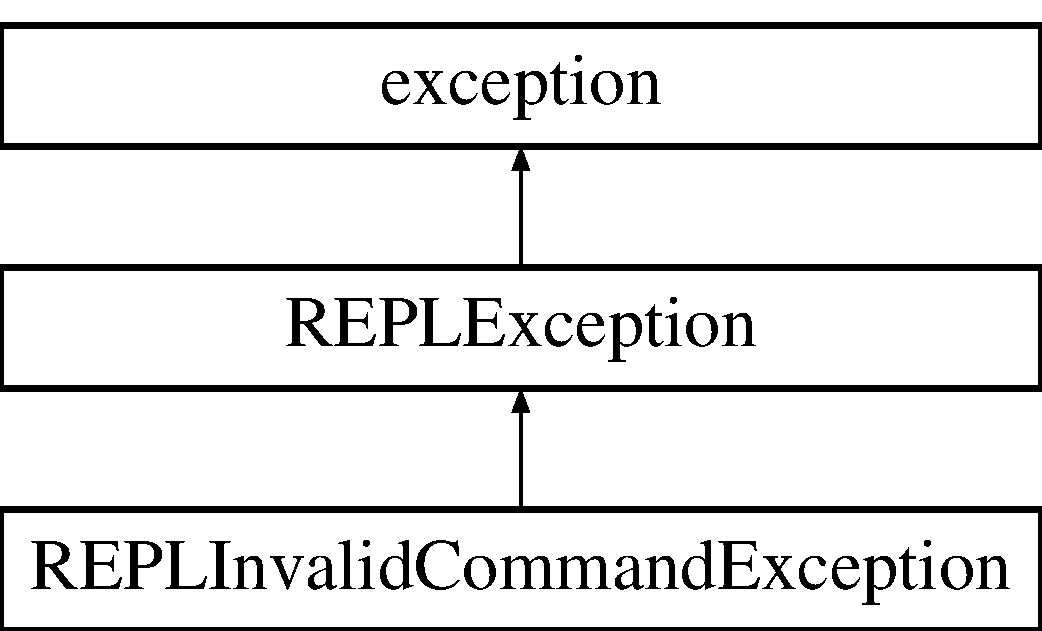
\includegraphics[height=3.000000cm]{classREPLInvalidCommandException}
\end{center}
\end{figure}
\doxysubsection*{Membros públicos}
\begin{DoxyCompactItemize}
\item 
\mbox{\Hypertarget{classREPLInvalidCommandException_add845747cce364d6144985faae0ec16a}\label{classREPLInvalidCommandException_add845747cce364d6144985faae0ec16a}} 
\mbox{\hyperlink{classREPLInvalidCommandException_add845747cce364d6144985faae0ec16a}{R\+E\+P\+L\+Invalid\+Command\+Exception}} ()
\begin{DoxyCompactList}\small\item\em Construtor de exceções de comando inválido. \end{DoxyCompactList}\item 
\mbox{\Hypertarget{classREPLInvalidCommandException_aec4c314ef19ce522dedb49c7451bafc0}\label{classREPLInvalidCommandException_aec4c314ef19ce522dedb49c7451bafc0}} 
const char $\ast$ \mbox{\hyperlink{classREPLInvalidCommandException_aec4c314ef19ce522dedb49c7451bafc0}{what}} () const  throw ()
\begin{DoxyCompactList}\small\item\em Retorna a mensagem de erro da exceção. \end{DoxyCompactList}\end{DoxyCompactItemize}


\doxysubsection{Descrição detalhada}
Classe de exceções de comando inválido. 

A documentação para esta classe foi gerada a partir do seguinte ficheiro\+:\begin{DoxyCompactItemize}
\item 
include/controllers/repl/\mbox{\hyperlink{Repl_8hpp}{Repl.\+hpp}}\end{DoxyCompactItemize}

\hypertarget{classREPLVertexNotFoundException}{}\doxysection{Referência à classe R\+E\+P\+L\+Vertex\+Not\+Found\+Exception}
\label{classREPLVertexNotFoundException}\index{REPLVertexNotFoundException@{REPLVertexNotFoundException}}


Classe de exceções de vértice não encontrado.  




{\ttfamily \#include $<$Repl.\+hpp$>$}

Diagrama de heranças da classe R\+E\+P\+L\+Vertex\+Not\+Found\+Exception\begin{figure}[H]
\begin{center}
\leavevmode
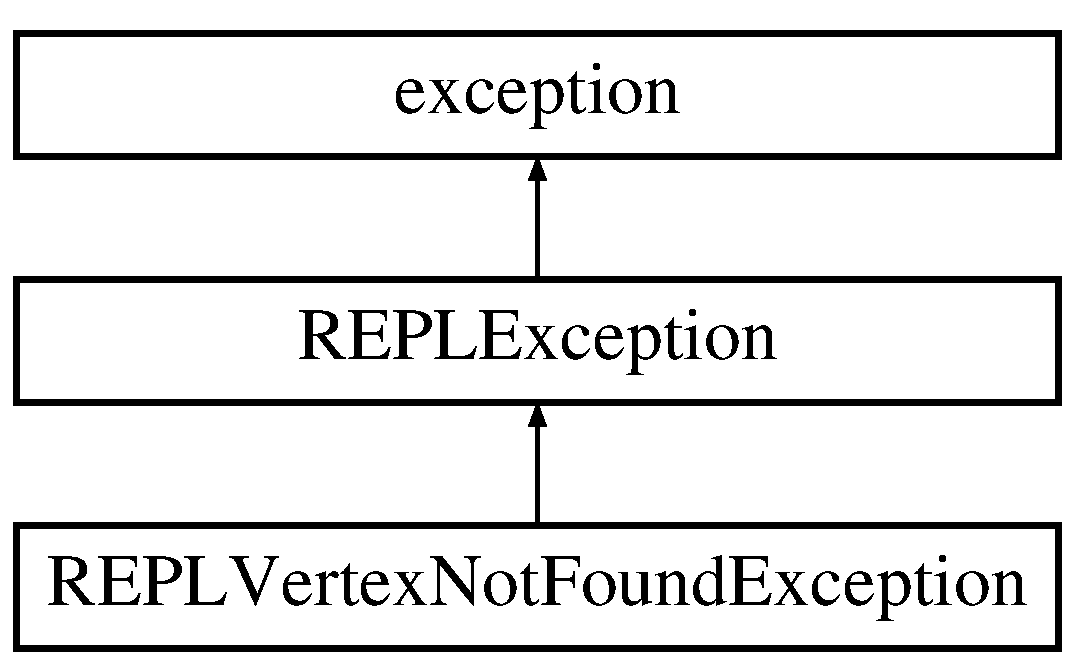
\includegraphics[height=3.000000cm]{classREPLVertexNotFoundException}
\end{center}
\end{figure}
\doxysubsection*{Membros públicos}
\begin{DoxyCompactItemize}
\item 
\mbox{\hyperlink{classREPLVertexNotFoundException_a30fcae3c8ffc5c861cab7474bbf5f658}{R\+E\+P\+L\+Vertex\+Not\+Found\+Exception}} (string v)
\item 
\mbox{\Hypertarget{classREPLVertexNotFoundException_ab8d189e6c0fcf90c87b4209096c45b53}\label{classREPLVertexNotFoundException_ab8d189e6c0fcf90c87b4209096c45b53}} 
const char $\ast$ \mbox{\hyperlink{classREPLVertexNotFoundException_ab8d189e6c0fcf90c87b4209096c45b53}{what}} () const  throw ()
\begin{DoxyCompactList}\small\item\em Retorna a mensagem de erro da exceção. \end{DoxyCompactList}\end{DoxyCompactItemize}


\doxysubsection{Descrição detalhada}
Classe de exceções de vértice não encontrado. 

\doxysubsection{Documentação dos Construtores \& Destrutor}
\mbox{\Hypertarget{classREPLVertexNotFoundException_a30fcae3c8ffc5c861cab7474bbf5f658}\label{classREPLVertexNotFoundException_a30fcae3c8ffc5c861cab7474bbf5f658}} 
\index{REPLVertexNotFoundException@{REPLVertexNotFoundException}!REPLVertexNotFoundException@{REPLVertexNotFoundException}}
\index{REPLVertexNotFoundException@{REPLVertexNotFoundException}!REPLVertexNotFoundException@{REPLVertexNotFoundException}}
\doxysubsubsection{\texorpdfstring{REPLVertexNotFoundException()}{REPLVertexNotFoundException()}}
{\footnotesize\ttfamily R\+E\+P\+L\+Vertex\+Not\+Found\+Exception\+::\+R\+E\+P\+L\+Vertex\+Not\+Found\+Exception (\begin{DoxyParamCaption}\item[{string}]{v }\end{DoxyParamCaption})\hspace{0.3cm}{\ttfamily [inline]}}

Construtor de exceções de vértice não encontrado. 
\begin{DoxyParams}{Parâmetros}
{\em string} & v que é o label de um vértice \\
\hline
\end{DoxyParams}
\begin{DoxyReturn}{Retorna}
mensagem de erro da exceção 
\end{DoxyReturn}


A documentação para esta classe foi gerada a partir do seguinte ficheiro\+:\begin{DoxyCompactItemize}
\item 
include/controllers/repl/\mbox{\hyperlink{Repl_8hpp}{Repl.\+hpp}}\end{DoxyCompactItemize}

\hypertarget{classTree}{}\doxysection{Referência à classe Tree}
\label{classTree}\index{Tree@{Tree}}


Classe para árvores.  




{\ttfamily \#include $<$Tree.\+hpp$>$}

Diagrama de heranças da classe Tree\begin{figure}[H]
\begin{center}
\leavevmode
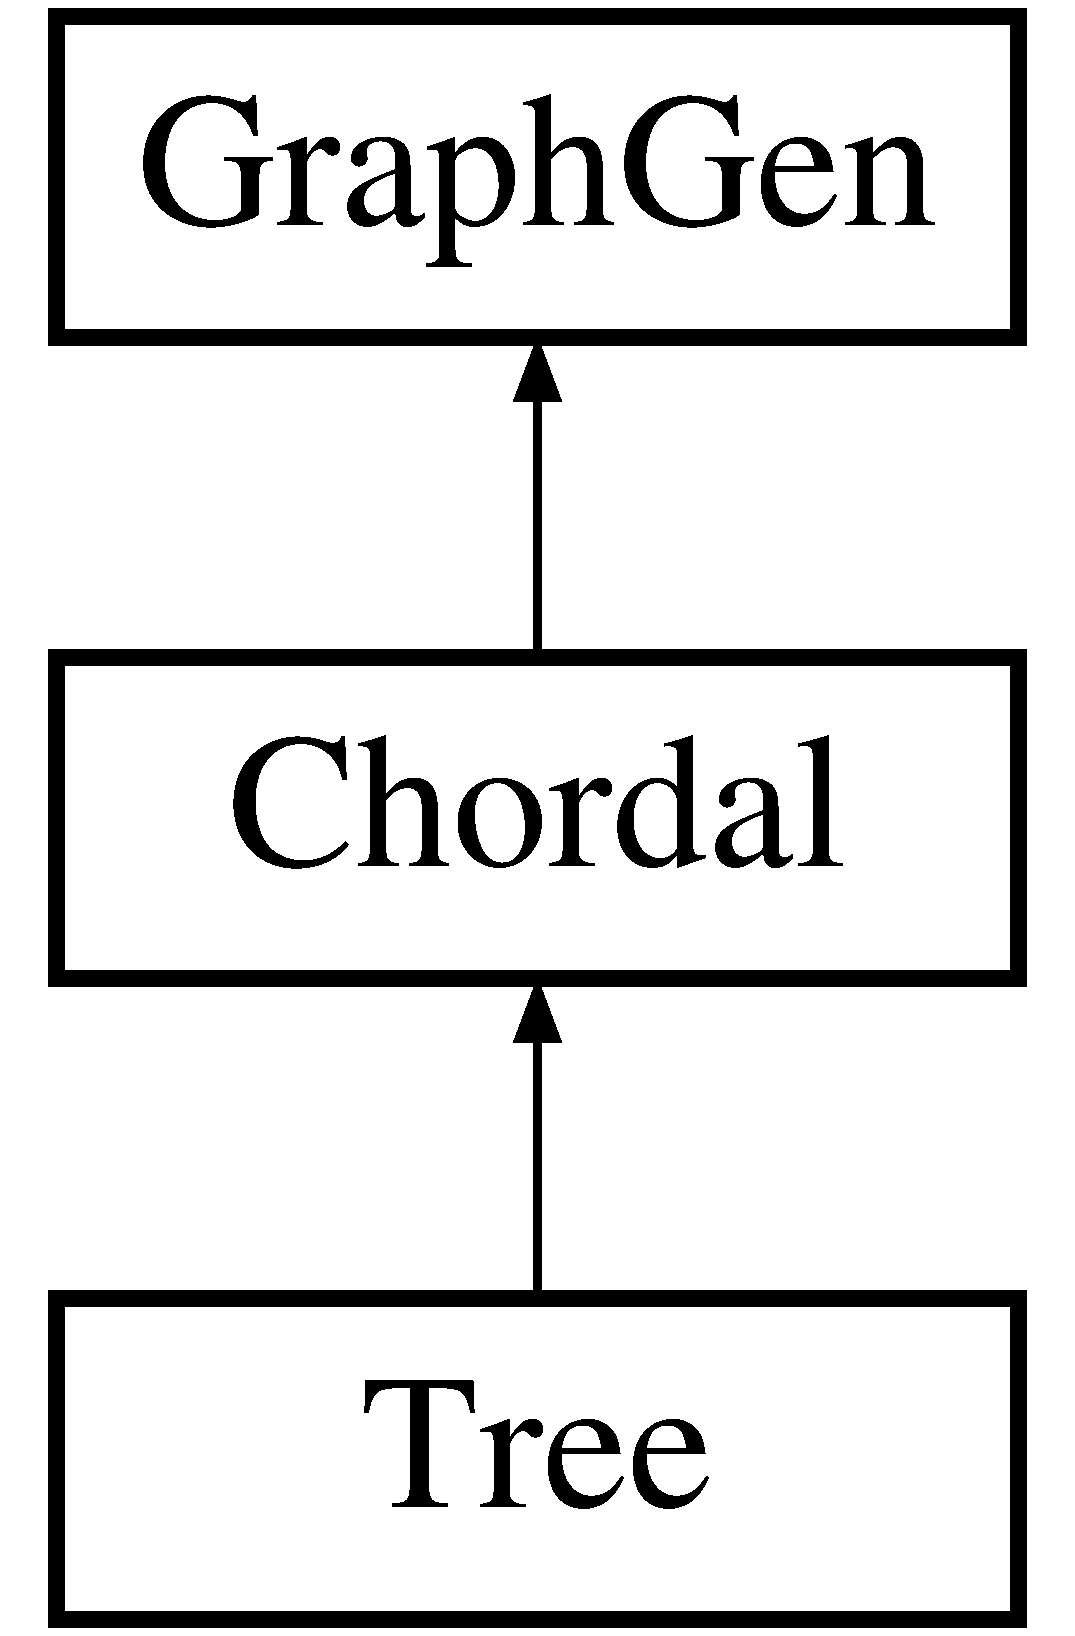
\includegraphics[height=3.000000cm]{classTree}
\end{center}
\end{figure}
\doxysubsection*{Membros públicos}
\begin{DoxyCompactItemize}
\item 
\mbox{\Hypertarget{classTree_ad376a7c639d857312f5de2ef47482f68}\label{classTree_ad376a7c639d857312f5de2ef47482f68}} 
\mbox{\hyperlink{classTree_ad376a7c639d857312f5de2ef47482f68}{Tree}} ()
\begin{DoxyCompactList}\small\item\em Construtor de árvores vazias. ~\newline
 \end{DoxyCompactList}\item 
\mbox{\Hypertarget{classTree_a25977c120f94e833fdd7739daa9b8d89}\label{classTree_a25977c120f94e833fdd7739daa9b8d89}} 
\mbox{\hyperlink{classTree_a25977c120f94e833fdd7739daa9b8d89}{Tree}} (int)
\begin{DoxyCompactList}\small\item\em Construtor de árvores por número de vértices. \end{DoxyCompactList}\item 
\mbox{\Hypertarget{classTree_a9f7d6a13c19b6525ee504079a5ffbd8e}\label{classTree_a9f7d6a13c19b6525ee504079a5ffbd8e}} 
\mbox{\hyperlink{classTree_a9f7d6a13c19b6525ee504079a5ffbd8e}{Tree}} (\mbox{\hyperlink{classGraphGen}{Graph\+Gen}} \&)
\begin{DoxyCompactList}\small\item\em Construtor de árvores por \mbox{\hyperlink{classGraphGen}{Graph\+Gen}}. \end{DoxyCompactList}\end{DoxyCompactItemize}
\doxysubsection*{Outros membros herdados}


\doxysubsection{Descrição detalhada}
Classe para árvores. 

A documentação para esta classe foi gerada a partir do seguinte ficheiro\+:\begin{DoxyCompactItemize}
\item 
include/models/graph/\mbox{\hyperlink{Tree_8hpp}{Tree.\+hpp}}\end{DoxyCompactItemize}

\hypertarget{classTreeConstructorException}{}\section{Referência à classe Tree\+Constructor\+Exception}
\label{classTreeConstructorException}\index{Tree\+Constructor\+Exception@{Tree\+Constructor\+Exception}}


Classe de exceções de construção de árvores.  




{\ttfamily \#include $<$Tree.\+hpp$>$}

Diagrama de heranças da classe Tree\+Constructor\+Exception\begin{figure}[H]
\begin{center}
\leavevmode
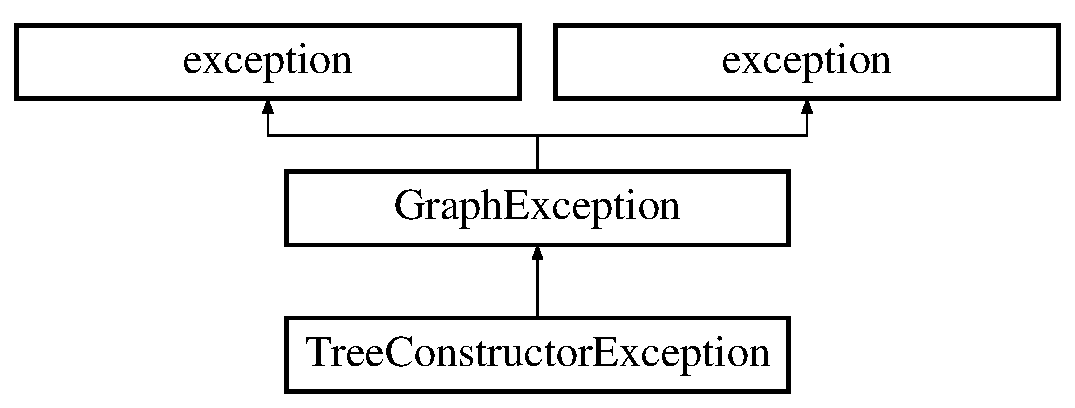
\includegraphics[height=3.000000cm]{classTreeConstructorException}
\end{center}
\end{figure}
\subsection*{Membros públicos}
\begin{DoxyCompactItemize}
\item 
\mbox{\Hypertarget{classTreeConstructorException_a2ecb31ba568ce3480ef9db767468f310}\label{classTreeConstructorException_a2ecb31ba568ce3480ef9db767468f310}} 
\hyperlink{classTreeConstructorException_a2ecb31ba568ce3480ef9db767468f310}{Tree\+Constructor\+Exception} ()
\begin{DoxyCompactList}\small\item\em Construtor da exceção. \end{DoxyCompactList}\item 
const char $\ast$ \hyperlink{classTreeConstructorException_acc8b569a2ad401614e1d8a9f6b0bd5d8}{what} () const  throw ()
\end{DoxyCompactItemize}


\subsection{Descrição detalhada}
Classe de exceções de construção de árvores. 

\subsection{Documentação dos métodos}
\mbox{\Hypertarget{classTreeConstructorException_acc8b569a2ad401614e1d8a9f6b0bd5d8}\label{classTreeConstructorException_acc8b569a2ad401614e1d8a9f6b0bd5d8}} 
\index{Tree\+Constructor\+Exception@{Tree\+Constructor\+Exception}!what@{what}}
\index{what@{what}!Tree\+Constructor\+Exception@{Tree\+Constructor\+Exception}}
\subsubsection{\texorpdfstring{what()}{what()}}
{\footnotesize\ttfamily const char$\ast$ Tree\+Constructor\+Exception\+::what (\begin{DoxyParamCaption}{ }\end{DoxyParamCaption}) const throw  ) \hspace{0.3cm}{\ttfamily [inline]}}

Retorna a mensagem de erro da exceção. \begin{DoxyReturn}{Retorna}
Mensagem de erro. 
\end{DoxyReturn}


A documentação para esta classe foi gerada a partir do seguinte ficheiro\+:\begin{DoxyCompactItemize}
\item 
include/models/graph/\hyperlink{Tree_8hpp}{Tree.\+hpp}\end{DoxyCompactItemize}

\hypertarget{classVector}{}\doxysection{Referência à classe Vector}
\label{classVector}\index{Vector@{Vector}}


Classe para operações vetoriais no espaço real de duas dimensões.  




{\ttfamily \#include $<$Vector.\+hpp$>$}

\doxysubsection*{Membros públicos}
\begin{DoxyCompactItemize}
\item 
\mbox{\Hypertarget{classVector_a6f80c73b5f18dcf3f8e36065bdc8b9e5}\label{classVector_a6f80c73b5f18dcf3f8e36065bdc8b9e5}} 
\mbox{\hyperlink{classVector_a6f80c73b5f18dcf3f8e36065bdc8b9e5}{Vector}} ()
\begin{DoxyCompactList}\small\item\em Construtor do vetor zero;. \end{DoxyCompactList}\item 
\mbox{\Hypertarget{classVector_a1d3e69fe5741740aa40e7b5fd2cbf0e8}\label{classVector_a1d3e69fe5741740aa40e7b5fd2cbf0e8}} 
\mbox{\hyperlink{classVector_a1d3e69fe5741740aa40e7b5fd2cbf0e8}{Vector}} (float, float)
\begin{DoxyCompactList}\small\item\em Construtor do vetor pelas posições x e y. \end{DoxyCompactList}\item 
\mbox{\Hypertarget{classVector_abdb4dca6245e33a8661d1ab02bb50016}\label{classVector_abdb4dca6245e33a8661d1ab02bb50016}} 
\mbox{\hyperlink{classVector_abdb4dca6245e33a8661d1ab02bb50016}{Vector}} (pair$<$ float, float $>$)
\begin{DoxyCompactList}\small\item\em Construtor do vetor por par de posições. \end{DoxyCompactList}\item 
\mbox{\Hypertarget{classVector_a4d643a71ea7c87cb77ab7bdfb26b42ba}\label{classVector_a4d643a71ea7c87cb77ab7bdfb26b42ba}} 
float \mbox{\hyperlink{classVector_a4d643a71ea7c87cb77ab7bdfb26b42ba}{norm}} ()
\begin{DoxyCompactList}\small\item\em Calcula a norma do vetor. \end{DoxyCompactList}\item 
\mbox{\Hypertarget{classVector_ac83edd3ce21c2eea555a360f64cf0acc}\label{classVector_ac83edd3ce21c2eea555a360f64cf0acc}} 
float \mbox{\hyperlink{classVector_ac83edd3ce21c2eea555a360f64cf0acc}{angle}} ()
\begin{DoxyCompactList}\small\item\em Calcula o ângulo do vetor com o eixo x. \end{DoxyCompactList}\item 
\mbox{\Hypertarget{classVector_ac2e3094ce0134c3509ce4ef7df78245a}\label{classVector_ac2e3094ce0134c3509ce4ef7df78245a}} 
\mbox{\hyperlink{classVector}{Vector}} \mbox{\hyperlink{classVector_ac2e3094ce0134c3509ce4ef7df78245a}{rotate}} (float)
\begin{DoxyCompactList}\small\item\em Rotaciona o vetor em um dado ângulo. \end{DoxyCompactList}\item 
\mbox{\Hypertarget{classVector_a7f187d9dc1da47c2d3754e8260a4c0e7}\label{classVector_a7f187d9dc1da47c2d3754e8260a4c0e7}} 
\mbox{\hyperlink{classVector}{Vector}} \mbox{\hyperlink{classVector_a7f187d9dc1da47c2d3754e8260a4c0e7}{project}} (\mbox{\hyperlink{classVector}{Vector}})
\begin{DoxyCompactList}\small\item\em Projeção do vetor sobre um outro vetor. \end{DoxyCompactList}\end{DoxyCompactItemize}
\doxysubsection*{Atributos Públicos}
\begin{DoxyCompactItemize}
\item 
\mbox{\Hypertarget{classVector_aca49165049a1e21ae47afcfc078819ed}\label{classVector_aca49165049a1e21ae47afcfc078819ed}} 
float \mbox{\hyperlink{classVector_aca49165049a1e21ae47afcfc078819ed}{x}}
\begin{DoxyCompactList}\small\item\em Coordenada x do vetor. \end{DoxyCompactList}\item 
\mbox{\Hypertarget{classVector_a81be9102fca6d9beea3efef522c4c09d}\label{classVector_a81be9102fca6d9beea3efef522c4c09d}} 
float \mbox{\hyperlink{classVector_a81be9102fca6d9beea3efef522c4c09d}{y}}
\begin{DoxyCompactList}\small\item\em Coordenada y do vetor. \end{DoxyCompactList}\end{DoxyCompactItemize}


\doxysubsection{Descrição detalhada}
Classe para operações vetoriais no espaço real de duas dimensões. 

A documentação para esta classe foi gerada a partir do seguinte ficheiro\+:\begin{DoxyCompactItemize}
\item 
include/models/data\+Structures/\mbox{\hyperlink{Vector_8hpp}{Vector.\+hpp}}\end{DoxyCompactItemize}

\chapter{Documentação do ficheiro}
\hypertarget{Repl_8hpp}{}\section{Referência ao ficheiro include/controllers/repl/\+Repl.hpp}
\label{Repl_8hpp}\index{include/controllers/repl/\+Repl.\+hpp@{include/controllers/repl/\+Repl.\+hpp}}
{\ttfamily \#include \char`\"{}Bipartite.\+hpp\char`\"{}}\newline
{\ttfamily \#include \char`\"{}Chordal.\+hpp\char`\"{}}\newline
{\ttfamily \#include \char`\"{}Dag.\+hpp\char`\"{}}\newline
{\ttfamily \#include \char`\"{}Graph.\+hpp\char`\"{}}\newline
{\ttfamily \#include \char`\"{}Graph\+Canvas.\+hpp\char`\"{}}\newline
{\ttfamily \#include \char`\"{}Interface.\+hpp\char`\"{}}\newline
{\ttfamily \#include \char`\"{}Tree.\+hpp\char`\"{}}\newline
{\ttfamily \#include $<$fstream$>$}\newline
{\ttfamily \#include $<$iostream$>$}\newline
{\ttfamily \#include $<$sstream$>$}\newline
{\ttfamily \#include $<$string$>$}\newline
\subsection*{Componentes}
\begin{DoxyCompactItemize}
\item 
class \hyperlink{classREPLException}{R\+E\+P\+L\+Exception}
\begin{DoxyCompactList}\small\item\em Classe para exceções do R\+E\+PL. \end{DoxyCompactList}\item 
class \hyperlink{classREPLInvalidCommandException}{R\+E\+P\+L\+Invalid\+Command\+Exception}
\begin{DoxyCompactList}\small\item\em Classe de exceções de comando inválido. \end{DoxyCompactList}\item 
class \hyperlink{classREPLVertexNotFoundException}{R\+E\+P\+L\+Vertex\+Not\+Found\+Exception}
\begin{DoxyCompactList}\small\item\em Classe de exceções de vértice não encontrado. \end{DoxyCompactList}\end{DoxyCompactItemize}
\subsection*{Funções}
\begin{DoxyCompactItemize}
\item 
\mbox{\Hypertarget{Repl_8hpp_a0719f91c310a88684005cfbdaf2d22a6}\label{Repl_8hpp_a0719f91c310a88684005cfbdaf2d22a6}} 
void {\bfseries repl\+::run} (int, int)
\end{DoxyCompactItemize}

\hypertarget{DSU_8hpp}{}\doxysection{Referência ao ficheiro include/models/data\+Structures/\+D\+SU.hpp}
\label{DSU_8hpp}\index{include/models/dataStructures/DSU.hpp@{include/models/dataStructures/DSU.hpp}}
{\ttfamily \#include $<$iostream$>$}\newline
{\ttfamily \#include $<$string$>$}\newline
{\ttfamily \#include $<$vector$>$}\newline
\doxysubsection*{Componentes}
\begin{DoxyCompactItemize}
\item 
class \mbox{\hyperlink{classDSU}{D\+SU}}
\begin{DoxyCompactList}\small\item\em Classe para Disjoint Set Union (\mbox{\hyperlink{classDSU}{D\+SU}}). \end{DoxyCompactList}\item 
class \mbox{\hyperlink{classDSUException}{D\+S\+U\+Exception}}
\begin{DoxyCompactList}\small\item\em Classe de exceções de \mbox{\hyperlink{classDSU}{D\+SU}}. \end{DoxyCompactList}\item 
class \mbox{\hyperlink{classDSUNegativeConstructorParameterException}{D\+S\+U\+Negative\+Constructor\+Parameter\+Exception}}
\begin{DoxyCompactList}\small\item\em Classe de exceções de parâmetro negativo no construtor. \end{DoxyCompactList}\item 
class \mbox{\hyperlink{classDSUValueOutOfBoundsException}{D\+S\+U\+Value\+Out\+Of\+Bounds\+Exception}}
\begin{DoxyCompactList}\small\item\em Classe de exceções de valor fora do range válido. \end{DoxyCompactList}\end{DoxyCompactItemize}

\hypertarget{Vector_8hpp}{}\section{Referência ao ficheiro include/models/data\+Structures/\+Vector.hpp}
\label{Vector_8hpp}\index{include/models/data\+Structures/\+Vector.\+hpp@{include/models/data\+Structures/\+Vector.\+hpp}}
{\ttfamily \#include $<$cmath$>$}\newline
{\ttfamily \#include $<$utility$>$}\newline
\subsection*{Componentes}
\begin{DoxyCompactItemize}
\item 
class \hyperlink{classVector}{Vector}
\begin{DoxyCompactList}\small\item\em Classe para operações vetoriais no espaço real de duas dimensões. \end{DoxyCompactList}\end{DoxyCompactItemize}
\subsection*{Funções}
\begin{DoxyCompactItemize}
\item 
\hyperlink{classVector}{Vector} \hyperlink{Vector_8hpp_af3fdd2b7487c71d4b20a74e30a95891d}{operator+} (const \hyperlink{classVector}{Vector} \&, const \hyperlink{classVector}{Vector} \&)
\item 
\hyperlink{classVector}{Vector} \hyperlink{Vector_8hpp_ac4505f13a01e5d3312660626ae4ddebb}{operator-\/} (const \hyperlink{classVector}{Vector} \&, const \hyperlink{classVector}{Vector} \&)
\item 
\hyperlink{classVector}{Vector} \hyperlink{Vector_8hpp_aa5ef2bdf4be5b94bbeafa5798bca75f2}{operator$\ast$} (const \hyperlink{classVector}{Vector} \&, const float)
\item 
float \hyperlink{Vector_8hpp_a66cbb2d65533e33ab585e24924e9b698}{operator$\ast$} (const \hyperlink{classVector}{Vector} \&, const \hyperlink{classVector}{Vector} \&)
\item 
float \hyperlink{Vector_8hpp_a77c45342e920b482a7974f0baa52613b}{operator\%} (const \hyperlink{classVector}{Vector} \&, const \hyperlink{classVector}{Vector} \&)
\item 
float \hyperlink{Vector_8hpp_ad0936cb11a42495f130f83abbfad19b1}{operator$^\wedge$} (const \hyperlink{classVector}{Vector} \&, const \hyperlink{classVector}{Vector} \&)
\end{DoxyCompactItemize}


\subsection{Documentação das funções}
\mbox{\Hypertarget{Vector_8hpp_a77c45342e920b482a7974f0baa52613b}\label{Vector_8hpp_a77c45342e920b482a7974f0baa52613b}} 
\index{Vector.\+hpp@{Vector.\+hpp}!operator\%@{operator\%}}
\index{operator\%@{operator\%}!Vector.\+hpp@{Vector.\+hpp}}
\subsubsection{\texorpdfstring{operator\%()}{operator\%()}}
{\footnotesize\ttfamily float operator\% (\begin{DoxyParamCaption}\item[{const \hyperlink{classVector}{Vector} \&}]{,  }\item[{const \hyperlink{classVector}{Vector} \&}]{ }\end{DoxyParamCaption})}

Produto vetorial entre vetores. 
\begin{DoxyParams}{Parâmetros}
{\em Vetores} & a serem multiplicados. \\
\hline
\end{DoxyParams}
\begin{DoxyReturn}{Retorna}
\hyperlink{classVector}{Vector} resultante. 
\end{DoxyReturn}
\mbox{\Hypertarget{Vector_8hpp_aa5ef2bdf4be5b94bbeafa5798bca75f2}\label{Vector_8hpp_aa5ef2bdf4be5b94bbeafa5798bca75f2}} 
\index{Vector.\+hpp@{Vector.\+hpp}!operator$\ast$@{operator$\ast$}}
\index{operator$\ast$@{operator$\ast$}!Vector.\+hpp@{Vector.\+hpp}}
\subsubsection{\texorpdfstring{operator$\ast$()}{operator*()}\hspace{0.1cm}{\footnotesize\ttfamily [1/2]}}
{\footnotesize\ttfamily \hyperlink{classVector}{Vector} operator$\ast$ (\begin{DoxyParamCaption}\item[{const \hyperlink{classVector}{Vector} \&}]{,  }\item[{const float}]{ }\end{DoxyParamCaption})}

Multiplicação de um vetor por um escalar. 
\begin{DoxyParams}{Parâmetros}
{\em \hyperlink{classVector}{Vector}} & a ser multiplicado. \\
\hline
{\em Escalar} & a se multiplicar. \\
\hline
\end{DoxyParams}
\begin{DoxyReturn}{Retorna}
\hyperlink{classVector}{Vector} resultante. 
\end{DoxyReturn}
\mbox{\Hypertarget{Vector_8hpp_a66cbb2d65533e33ab585e24924e9b698}\label{Vector_8hpp_a66cbb2d65533e33ab585e24924e9b698}} 
\index{Vector.\+hpp@{Vector.\+hpp}!operator$\ast$@{operator$\ast$}}
\index{operator$\ast$@{operator$\ast$}!Vector.\+hpp@{Vector.\+hpp}}
\subsubsection{\texorpdfstring{operator$\ast$()}{operator*()}\hspace{0.1cm}{\footnotesize\ttfamily [2/2]}}
{\footnotesize\ttfamily float operator$\ast$ (\begin{DoxyParamCaption}\item[{const \hyperlink{classVector}{Vector} \&}]{,  }\item[{const \hyperlink{classVector}{Vector} \&}]{ }\end{DoxyParamCaption})}

Produto escalar entre vetores. 
\begin{DoxyParams}{Parâmetros}
{\em Vetores} & a serem multiplicados. \\
\hline
\end{DoxyParams}
\begin{DoxyReturn}{Retorna}
\hyperlink{classVector}{Vector} resultante. 
\end{DoxyReturn}
\mbox{\Hypertarget{Vector_8hpp_af3fdd2b7487c71d4b20a74e30a95891d}\label{Vector_8hpp_af3fdd2b7487c71d4b20a74e30a95891d}} 
\index{Vector.\+hpp@{Vector.\+hpp}!operator+@{operator+}}
\index{operator+@{operator+}!Vector.\+hpp@{Vector.\+hpp}}
\subsubsection{\texorpdfstring{operator+()}{operator+()}}
{\footnotesize\ttfamily \hyperlink{classVector}{Vector} operator+ (\begin{DoxyParamCaption}\item[{const \hyperlink{classVector}{Vector} \&}]{,  }\item[{const \hyperlink{classVector}{Vector} \&}]{ }\end{DoxyParamCaption})}

Soma de vetores. 
\begin{DoxyParams}{Parâmetros}
{\em Vetores} & a serem somados. \\
\hline
\end{DoxyParams}
\begin{DoxyReturn}{Retorna}
\hyperlink{classVector}{Vector} resultante. 
\end{DoxyReturn}
\mbox{\Hypertarget{Vector_8hpp_ac4505f13a01e5d3312660626ae4ddebb}\label{Vector_8hpp_ac4505f13a01e5d3312660626ae4ddebb}} 
\index{Vector.\+hpp@{Vector.\+hpp}!operator-\/@{operator-\/}}
\index{operator-\/@{operator-\/}!Vector.\+hpp@{Vector.\+hpp}}
\subsubsection{\texorpdfstring{operator-\/()}{operator-()}}
{\footnotesize\ttfamily \hyperlink{classVector}{Vector} operator-\/ (\begin{DoxyParamCaption}\item[{const \hyperlink{classVector}{Vector} \&}]{,  }\item[{const \hyperlink{classVector}{Vector} \&}]{ }\end{DoxyParamCaption})}

Subtração de vetores. 
\begin{DoxyParams}{Parâmetros}
{\em Vetores} & a serem subtraídos. \\
\hline
\end{DoxyParams}
\begin{DoxyReturn}{Retorna}
\hyperlink{classVector}{Vector} resultante. 
\end{DoxyReturn}
\mbox{\Hypertarget{Vector_8hpp_ad0936cb11a42495f130f83abbfad19b1}\label{Vector_8hpp_ad0936cb11a42495f130f83abbfad19b1}} 
\index{Vector.\+hpp@{Vector.\+hpp}!operator$^\wedge$@{operator$^\wedge$}}
\index{operator$^\wedge$@{operator$^\wedge$}!Vector.\+hpp@{Vector.\+hpp}}
\subsubsection{\texorpdfstring{operator$^\wedge$()}{operator^()}}
{\footnotesize\ttfamily float operator$^\wedge$ (\begin{DoxyParamCaption}\item[{const \hyperlink{classVector}{Vector} \&}]{,  }\item[{const \hyperlink{classVector}{Vector} \&}]{ }\end{DoxyParamCaption})}

Distância normalizada entre vetores. 
\begin{DoxyParams}{Parâmetros}
{\em Vetores} & a se calcular a distância. \\
\hline
\end{DoxyParams}
\begin{DoxyReturn}{Retorna}
Distância entre eles. 
\end{DoxyReturn}

\hypertarget{Bipartite_8hpp}{}\doxysection{Referência ao ficheiro include/models/graph/\+Bipartite.hpp}
\label{Bipartite_8hpp}\index{include/models/graph/Bipartite.hpp@{include/models/graph/Bipartite.hpp}}
{\ttfamily \#include \char`\"{}Graph\+Gen.\+hpp\char`\"{}}\newline
\doxysubsection*{Componentes}
\begin{DoxyCompactItemize}
\item 
class \mbox{\hyperlink{classBipartite}{Bipartite}}
\begin{DoxyCompactList}\small\item\em Classe para grafos bipartidos. \end{DoxyCompactList}\item 
class \mbox{\hyperlink{classBipartiteConstructorException}{Bipartite\+Constructor\+Exception}}
\begin{DoxyCompactList}\small\item\em Classe de exceções de construção de grafos bipartidos. \end{DoxyCompactList}\end{DoxyCompactItemize}

\hypertarget{Chordal_8hpp}{}\section{Referência ao ficheiro include/models/graph/\+Chordal.hpp}
\label{Chordal_8hpp}\index{include/models/graph/\+Chordal.\+hpp@{include/models/graph/\+Chordal.\+hpp}}
{\ttfamily \#include \char`\"{}Graph\+Gen.\+hpp\char`\"{}}\newline
\subsection*{Componentes}
\begin{DoxyCompactItemize}
\item 
class \hyperlink{classChordal}{Chordal}
\begin{DoxyCompactList}\small\item\em Classe para grafos cordais. \end{DoxyCompactList}\item 
class \hyperlink{classChordalConstructorException}{Chordal\+Constructor\+Exception}
\begin{DoxyCompactList}\small\item\em Classe de exceções de construção de grafos cordais. \end{DoxyCompactList}\end{DoxyCompactItemize}

\hypertarget{Dag_8hpp}{}\doxysection{Referência ao ficheiro include/models/graph/\+Dag.hpp}
\label{Dag_8hpp}\index{include/models/graph/Dag.hpp@{include/models/graph/Dag.hpp}}
{\ttfamily \#include \char`\"{}Graph\+Gen.\+hpp\char`\"{}}\newline
\doxysubsection*{Componentes}
\begin{DoxyCompactItemize}
\item 
class \mbox{\hyperlink{classDag}{Dag}}
\begin{DoxyCompactList}\small\item\em Classe para grafos direcionados acíclicos. \end{DoxyCompactList}\item 
class \mbox{\hyperlink{classDagConstructorException}{Dag\+Constructor\+Exception}}
\begin{DoxyCompactList}\small\item\em Classe de exceção de construção de D\+A\+Gs. \end{DoxyCompactList}\end{DoxyCompactItemize}

\hypertarget{Graph_8hpp}{}\doxysection{Referência ao ficheiro include/models/graph/\+Graph.hpp}
\label{Graph_8hpp}\index{include/models/graph/Graph.hpp@{include/models/graph/Graph.hpp}}
{\ttfamily \#include \char`\"{}Bipartite.\+hpp\char`\"{}}\newline
{\ttfamily \#include \char`\"{}Chordal.\+hpp\char`\"{}}\newline
{\ttfamily \#include \char`\"{}D\+S\+U.\+hpp\char`\"{}}\newline
{\ttfamily \#include \char`\"{}Dag.\+hpp\char`\"{}}\newline
{\ttfamily \#include \char`\"{}Graph\+Gen.\+hpp\char`\"{}}\newline
{\ttfamily \#include \char`\"{}Tree.\+hpp\char`\"{}}\newline
{\ttfamily \#include $<$algorithm$>$}\newline
{\ttfamily \#include $<$iostream$>$}\newline
{\ttfamily \#include $<$string$>$}\newline
{\ttfamily \#include $<$vector$>$}\newline
\doxysubsection*{Componentes}
\begin{DoxyCompactItemize}
\item 
class \mbox{\hyperlink{classGraph}{Graph}}
\begin{DoxyCompactList}\small\item\em Classe para grafos. \end{DoxyCompactList}\item 
class \mbox{\hyperlink{classGraphVertexOutOfBoundsException}{Graph\+Vertex\+Out\+Of\+Bounds\+Exception}}
\begin{DoxyCompactList}\small\item\em Classe de exceções de vértice fora dos limites. \end{DoxyCompactList}\item 
class \mbox{\hyperlink{classGraphSelfLoopException}{Graph\+Self\+Loop\+Exception}}
\begin{DoxyCompactList}\small\item\em Classe de exceções de laços. \end{DoxyCompactList}\end{DoxyCompactItemize}

\hypertarget{GraphGen_8hpp}{}\doxysection{Referência ao ficheiro include/models/graph/\+Graph\+Gen.hpp}
\label{GraphGen_8hpp}\index{include/models/graph/GraphGen.hpp@{include/models/graph/GraphGen.hpp}}
{\ttfamily \#include $<$algorithm$>$}\newline
{\ttfamily \#include $<$iostream$>$}\newline
{\ttfamily \#include $<$numeric$>$}\newline
{\ttfamily \#include $<$queue$>$}\newline
{\ttfamily \#include $<$set$>$}\newline
{\ttfamily \#include $<$stack$>$}\newline
{\ttfamily \#include $<$string$>$}\newline
{\ttfamily \#include $<$utility$>$}\newline
{\ttfamily \#include $<$vector$>$}\newline
\doxysubsection*{Componentes}
\begin{DoxyCompactItemize}
\item 
class \mbox{\hyperlink{classGraphGen}{Graph\+Gen}}
\item 
class \mbox{\hyperlink{classGraphException}{Graph\+Exception}}
\begin{DoxyCompactList}\small\item\em Classe de exceções de grafos. \end{DoxyCompactList}\item 
class \mbox{\hyperlink{classGraphNoPathException}{Graph\+No\+Path\+Exception}}
\begin{DoxyCompactList}\small\item\em Classe de exceções de ausência de caminho entre dois vértices. \end{DoxyCompactList}\item 
class \mbox{\hyperlink{classGraphNegativeCycleException}{Graph\+Negative\+Cycle\+Exception}}
\begin{DoxyCompactList}\small\item\em Classe de exceções para ciclos negativos em caminhos mínimos. \end{DoxyCompactList}\item 
class \mbox{\hyperlink{classGraphOrderingException}{Graph\+Ordering\+Exception}}
\begin{DoxyCompactList}\small\item\em Classe de exceções para ordenações de vértices fora do domínio. \end{DoxyCompactList}\end{DoxyCompactItemize}


\doxysubsection{Descrição detalhada}
Classe para grafos gerais. 
\hypertarget{Tree_8hpp}{}\section{Referência ao ficheiro include/models/graph/\+Tree.hpp}
\label{Tree_8hpp}\index{include/models/graph/\+Tree.\+hpp@{include/models/graph/\+Tree.\+hpp}}
{\ttfamily \#include \char`\"{}Chordal.\+hpp\char`\"{}}\newline
\subsection*{Componentes}
\begin{DoxyCompactItemize}
\item 
class \hyperlink{classTree}{Tree}
\begin{DoxyCompactList}\small\item\em Classe para árvores. \end{DoxyCompactList}\item 
class \hyperlink{classTreeConstructorException}{Tree\+Constructor\+Exception}
\begin{DoxyCompactList}\small\item\em Classe de exceções de construção de árvores. \end{DoxyCompactList}\end{DoxyCompactItemize}

\hypertarget{GraphCanvas_8hpp}{}\section{Referência ao ficheiro include/views/\+Graph\+Canvas.hpp}
\label{GraphCanvas_8hpp}\index{include/views/\+Graph\+Canvas.\+hpp@{include/views/\+Graph\+Canvas.\+hpp}}
{\ttfamily \#include \char`\"{}Graph\+Display.\+hpp\char`\"{}}\newline
{\ttfamily \#include \char`\"{}Vector.\+hpp\char`\"{}}\newline
{\ttfamily \#include $<$S\+F\+M\+L/\+Graphics.\+hpp$>$}\newline
{\ttfamily \#include $<$fstream$>$}\newline
{\ttfamily \#include $<$iostream$>$}\newline
{\ttfamily \#include $<$sstream$>$}\newline
{\ttfamily \#include $<$string$>$}\newline
{\ttfamily \#include $<$utility$>$}\newline
{\ttfamily \#include $<$vector$>$}\newline
\subsection*{Componentes}
\begin{DoxyCompactItemize}
\item 
class \hyperlink{classGraphCanvas}{Graph\+Canvas}
\begin{DoxyCompactList}\small\item\em Classe para o canvas. \end{DoxyCompactList}\item 
class \hyperlink{classFileNotFoundException}{File\+Not\+Found\+Exception}
\begin{DoxyCompactList}\small\item\em Classe de exceções para leitura de grafos inexistentes. \end{DoxyCompactList}\end{DoxyCompactItemize}
\subsection*{Variáveis}
\begin{DoxyCompactItemize}
\item 
\mbox{\Hypertarget{GraphCanvas_8hpp_ab31acecc6d9911bb6c200924d00b5476}\label{GraphCanvas_8hpp_ab31acecc6d9911bb6c200924d00b5476}} 
\hyperlink{classGraph}{Graph} \hyperlink{GraphCanvas_8hpp_ab31acecc6d9911bb6c200924d00b5476}{ler\+Grafo\+Arquivo} (string)
\begin{DoxyCompactList}\small\item\em Retorna grafo lido de um dado arquivo. \end{DoxyCompactList}\end{DoxyCompactItemize}

\hypertarget{GraphDisplay_8hpp}{}\section{Referência ao ficheiro include/views/\+Graph\+Display.hpp}
\label{GraphDisplay_8hpp}\index{include/views/\+Graph\+Display.\+hpp@{include/views/\+Graph\+Display.\+hpp}}
{\ttfamily \#include \char`\"{}Graph.\+hpp\char`\"{}}\newline
{\ttfamily \#include \char`\"{}Vector.\+hpp\char`\"{}}\newline
{\ttfamily \#include $<$cmath$>$}\newline
{\ttfamily \#include $<$cstdlib$>$}\newline
{\ttfamily \#include $<$vector$>$}\newline
\subsection*{Componentes}
\begin{DoxyCompactItemize}
\item 
class \hyperlink{classGraphDisplay}{Graph\+Display}
\begin{DoxyCompactList}\small\item\em Classe para display do grafo. \end{DoxyCompactList}\end{DoxyCompactItemize}

%--- End generated contents ---

% Index
\backmatter
\newpage
\phantomsection
\clearemptydoublepage
\addcontentsline{toc}{chapter}{Índice}
\printindex

\end{document}
